\documentclass[11.5pt, a4paper]{scrartcl}
\usepackage[english]{babel}
\usepackage{fontspec}
\usepackage[top=35pt, left=2.25cm, right=2.2cm]{geometry}
\usepackage{setspace}
\usepackage{fancyhdr}
\pagestyle{fancy}
\fancyhf{moresize}
\usepackage{hyperref}
\usepackage{float}
\usepackage{multicol}
\usepackage[dvipsnames,table]{xcolor}
\usepackage{soul}
\usepackage{tikz}
\usetikzlibrary{calc}
\usepackage[placement=bottom,scale=1,opacity=1]{background}
\setlength{\headheight}{40pt}
\setlength{\footskip}{60pt}
\usepackage{eurosym}
\usepackage{booktabs}
\setlength{\heavyrulewidth}{1.5pt}
\setlength{\abovetopsep}{4pt}
\fancyhf{}
\fancyhead[R]{\small SVF STUDY - APRIL 2021}
\fancyfoot[R] { {\textcolor{white}\thepage}}
\fancypagestyle{plain}{%
\fancyhf{}
\fancyfoot[R] {\Large \thepage}
}
\definecolor{color0}{HTML}{FAE5D3}
\definecolor{color1}{HTML}{EDBB99}
\definecolor{color2}{HTML}{DC7633}
\definecolor{color3}{HTML}{BA4A00}
\definecolor{color4}{HTML}{873600}
\definecolor{mygreen1}{HTML}{6CAE33}
\definecolor{mygray}{HTML}{EAECEE}
\hypersetup{
    colorlinks,
    linkcolor={hederablue},
    citecolor={mygreen1!50!black},
    urlcolor={mygreen1!80!black}
}
\begin{document}
\definecolor{hederablue}{HTML}{283747}
\backgroundsetup{contents={%
\begin{tikzpicture}
\shade[left color=hederablue, middle color = hederablue, right color = hederablue] (0,1.3) rectangle (23,0);
\node (mytext) at (4.2,0.53) { {\textcolor{white}{\textsf{POWERED BY}}}};
\node (myfirstpic) at (6,0.33) {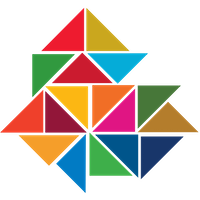
\includegraphics[height=.7cm]{/Users/chaix/Hedera/GIT/XLSform2PDF/code/assets/HEDERA.png}};
\end{tikzpicture}}
}
\setmainfont{Josefin Sans}
\setcounter{secnumdepth}{1}
\parindent 0pt
\tableofcontents

\vspace*{\fill}
\begin{minipage}[t]{0.7\textwidth}
{\small
\begin{flushleft}
HEDERA XLSForm$\_$Explore v1.0 (May 2021) \\[0.2em]
XLSForm$\_$Explore is an open source project to
automatically create a codebook from XLS Forms (view on \href{https://github.com/HEDERA-PLATFORM/XLSform2PDF}{github})\\
Survey: SVF STUDY - APRIL 2021\\
ID: svf$\_$study$\_$2021 -- version 20210326344\\
Data file: /Users/chaix/Hedera/GIT/XLSform2PDF/output/svf/svf$\_$study$\_$2021$\_$cleaned.csv (last update on: 28 April, 2021) \\
© Copyright \href{https://hedera.online}{HEDERA Sustainable Solutions}
\end{flushleft}
}\end{minipage}
\newpage\section{Identification}
\paragraph{Enumerator}
\  \\Variable name: \texttt{enumerator}\hfill\colorbox{red}{\small{\textcolor{white}{required}}}\\
 Type: single choice\\
\\Total number of answers: 245 (100.0\%)
\\[0.2em] \begin{tabular}{p{4cm}|p{8cm}|p{3cm}}
Choice code & Label & Answers \\
\hline
1 & Uwase Princesse& \cellcolor{color0}49 (20.0\%)\\
\cellcolor{mygray} 2 & \cellcolor{mygray}Gashakamba Octave & \cellcolor{color0}44 (18.0\%)\\
3 & Izere Ange Noelle& \cellcolor{color1}54 (22.0\%)\\
\cellcolor{mygray} 4 & \cellcolor{mygray}Jabukiro Kessy & \cellcolor{color0}49 (20.0\%)\\
5 & Mukakamana Valentine& \cellcolor{color0}49 (20.0\%)\\
\end{tabular}
\paragraph{Village}
\  \\Variable name: \texttt{village}\hfill\colorbox{red}{\small{\textcolor{white}{required}}}\\
 Type: single choice\\
\\Total number of answers: 245 (100.0\%)
\\[0.2em] \begin{tabular}{p{4cm}|p{8cm}|p{3cm}}
Choice code & Label & Answers \\
\hline
bisagara & Bisagara& \cellcolor{color2}131 (53.5\%)\\
\cellcolor{mygray} rugarama & \cellcolor{mygray}Rugarama & \cellcolor{color2}114 (46.5\%)\\
\end{tabular}
\newpage\section{Electricity Supply}
\paragraph{What is the main source of electricity used in the household?}
\  \\Variable name: \texttt{electricity\_source}\hfill\colorbox{red}{\small{\textcolor{white}{required}}}\\
 Type: single choice\\
\\Total number of answers: 245 (100.0\%)
\\[0.2em] \begin{tabular}{p{4cm}|p{8cm}|p{3cm}}
Choice code & Label & Answers \\
\hline
none & None& \cellcolor{color2}111 (45.3\%)\\
\cellcolor{mygray} shs & \cellcolor{mygray}Solar System & \cellcolor{color2}134 (54.7\%)\\
other & Other& \cellcolor{color0}0 (0.0\%)\\
\end{tabular}
\paragraph{Please specify the source of electricity:}
\  \\Variable name: \texttt{electricity\_source\_other}\hfill\colorbox{red}{\small{\textcolor{white}{required}}}\\
 Type: text\\
\\Total number of answers: 245 (100.0\%)
\\[0.2em]\paragraph{What do you mainly use for lighting?}
\  \\Variable name: \texttt{electricity\_illumination\_source}\hfill\colorbox{red}{\small{\textcolor{white}{required}}}\\
 Type: multiple choice\\
\\Total number of answers: 245 (100.0\%)
\\[0.2em] \begin{tabular}{p{4cm}|p{8cm}|p{3cm}}
Choice code & Label & Answers \\
\hline
none & None & \cellcolor{color0}2 (0.8\%)\\
\cellcolor{mygray} kerosene & \cellcolor{mygray}Kerosene lamp & \cellcolor{color0}0 (0.0\%)\\
candles & Candles& \cellcolor{color0}24 (9.8\%)\\
\cellcolor{mygray} solar\_torch & \cellcolor{mygray}Solar torch / Solar lantern / Solar desktop lamp & \cellcolor{color0}21 (8.6\%)\\
solar\_lamp & Solar lamp / Solar area floodlight& \cellcolor{color2}123 (50.2\%)\\
\cellcolor{mygray} torch\_battery & \cellcolor{mygray}Torch / Battery torch / Rechargeable battery flashlight & \cellcolor{color2}127 (51.8\%)\\
firewood & Firewood / Firelight& \cellcolor{color0}6 (2.4\%)\\
\cellcolor{mygray} other & \cellcolor{mygray}Other & \cellcolor{color0}1 (0.4\%)\\
\end{tabular}
\paragraph{Please specify:}
\  \\Variable name: \texttt{electricity\_illumination\_source\_other}\hfill\colorbox{red}{\small{\textcolor{white}{required}}}\\
 Type: text\\
\\Total number of answers: 245 (100.0\%)
\\[0.2em]\begin{table}[H]
 \begin{tabular}{p{4cm}|p{8cm}}
Word & Number of occurrences  \\
\hline
\cellcolor{mygray}guhambira&\cellcolor{mygray}1\\
\hline
amabuye&1\\
\hline
\cellcolor{mygray}radio&\cellcolor{mygray}1\\
\hline
ku&1\\
\hline
\cellcolor{mygray}mikoba&\cellcolor{mygray}1\\
\hline
\end{tabular}
\caption{\label{tab:table-name} Most used words for this answer}
\end{table}
\paragraph{If the household does not have any of the listed power sources, please specify any other source available.}
\  \\Variable name: \texttt{electricity\_no\_sources\_check}\\
Type: text\\
\\Total number of answers: 245 (100.0\%)
\\[0.2em]\begin{table}[H]
 \begin{tabular}{p{4cm}|p{8cm}}
Word & Number of occurrences  \\
\hline
\cellcolor{mygray}source&\cellcolor{mygray}2\\
\hline
power&1\\
\hline
\end{tabular}
\caption{\label{tab:table-name} Most used words for this answer}
\end{table}
\paragraph{Please indicate which electric appliances you have at home.}
\ \\ {\small Select all the options that apply.}
\  \\Variable name: \texttt{electricity\_appliances}\hfill\colorbox{red}{\small{\textcolor{white}{required}}}\\
 Type: multiple choice\\
\\Total number of answers: 245 (100.0\%)
\\[0.2em] \begin{tabular}{p{4cm}|p{8cm}|p{3cm}}
Choice code & Label & Answers \\
\hline
none & None& \cellcolor{color1}51 (20.8\%)\\
\cellcolor{mygray} mobile & \cellcolor{mygray}Basic mobile phones & \cellcolor{color3}191 (78.0\%)\\
smartphone\_offline & Smartphone without internet access& \cellcolor{color0}3 (1.2\%)\\
\cellcolor{mygray} smartphone & \cellcolor{mygray}Smartphone with internet access & \cellcolor{color0}6 (2.4\%)\\
satellite & Satellite dish& \cellcolor{color0}0 (0.0\%)\\
\cellcolor{mygray} tv  & \cellcolor{mygray}TV (color) & \cellcolor{color0}0 (0.0\%)\\
dvd & DVD& \cellcolor{color0}1 (0.4\%)\\
\cellcolor{mygray} radiu & \cellcolor{mygray}Radio & \cellcolor{color0}43 (17.6\%)\\
sound & Sound system& \cellcolor{color0}1 (0.4\%)\\
\cellcolor{mygray} charger & \cellcolor{mygray}Battery charger & \cellcolor{color0}0 (0.0\%)\\
fan & Fan& \cellcolor{color0}0 (0.0\%)\\
\cellcolor{mygray} water\_pump & \cellcolor{mygray}Water pump & \cellcolor{color0}0 (0.0\%)\\
other & Other& \cellcolor{color0}0 (0.0\%)\\
\end{tabular}
\paragraph{Please specify:}
\  \\Variable name: \texttt{electricity\_appliances\_other}\hfill\colorbox{red}{\small{\textcolor{white}{required}}}\\
 Type: text\\
\\Total number of answers: 245 (100.0\%)
\\[0.2em]\paragraph{When did you buy the solar system?}
\  \\Variable name: \texttt{solar\_system\_year}\hfill\colorbox{red}{\small{\textcolor{white}{required}}}\\
 Type: single choice\\
\\Total number of answers: 62 (25.3\%)
\\[0.2em] \begin{tabular}{p{4cm}|p{8cm}|p{3cm}}
Choice code & Label & Answers \\
\hline
2021 & 2021& \cellcolor{color0}7 (11.3\%)\\
\cellcolor{mygray} 2020 & \cellcolor{mygray}2020 & \cellcolor{color0}9 (14.5\%)\\
2019 & 2019& \cellcolor{color1}20 (32.3\%)\\
\cellcolor{mygray} 2018 & \cellcolor{mygray}2018 & \cellcolor{color0}9 (14.5\%)\\
2017 & 2017& \cellcolor{color0}6 (9.7\%)\\
\cellcolor{mygray} 2016 & \cellcolor{mygray}2016 & \cellcolor{color0}7 (11.3\%)\\
2015 & 2015& \cellcolor{color0}3 (4.8\%)\\
\cellcolor{mygray} 2014 & \cellcolor{mygray}2014 & \cellcolor{color0}0 (0.0\%)\\
before\_2014 & Before 2014& \cellcolor{color0}0 (0.0\%)\\
\cellcolor{mygray} na & \cellcolor{mygray}Don’t know & \cellcolor{color0}1 (1.6\%)\\
\end{tabular}
\paragraph{Is it possible to see the battery/control unit (where all the cables are connected to)) of the solar system? Can  I take a photo?}
\  \\Variable name: \texttt{solar\_system\_picture}\\
Type: image\\
\paragraph{Can you charge mobile phones with the electricity\_source\_label?}
\  \\Variable name: \texttt{solar\_system\_phones}\hfill\colorbox{red}{\small{\textcolor{white}{required}}}\\
 Type: single choice\\
\\Total number of answers: 136 (55.5\%)
\\[0.2em] \begin{tabular}{p{4cm}|p{8cm}|p{3cm}}
Choice code & Label & Answers \\
\hline
yes & Yes& \cellcolor{color3}107 (78.7\%)\\
\cellcolor{mygray} no & \cellcolor{mygray}No  & \cellcolor{color0}20 (14.7\%)\\
na & No mobile phone in the household& \cellcolor{color0}9 (6.6\%)\\
\end{tabular}
\paragraph{Can you charge mobile phones to full charge every day with the electricity\_source\_label?}
\  \\Variable name: \texttt{solar\_system\_phones\_full}\hfill\colorbox{red}{\small{\textcolor{white}{required}}}\\
 Type: single choice\\
\\Total number of answers: 107 (43.7\%)
\\[0.2em] \begin{tabular}{p{4cm}|p{8cm}|p{3cm}}
Choice code & Label & Answers \\
\hline
yes & Yes& \cellcolor{color4}100 (93.5\%)\\
\cellcolor{mygray} no & \cellcolor{mygray}No & \cellcolor{color0}7 (6.5\%)\\
\end{tabular}
\paragraph{You can add additional comments on the satisfaction with the solar device(s)}
\  \\Variable name: \texttt{solar\_additional\_comments}\\
Type: text\\
\\Total number of answers: 107 (43.7\%)
\\[0.2em]\begin{table}[H]
 \begin{tabular}{p{4cm}|p{8cm}}
Word & Number of occurrences  \\
\hline
\cellcolor{mygray}well&\cellcolor{mygray}37\\
\hline
system&35\\
\hline
\cellcolor{mygray}works&\cellcolor{mygray}22\\
\hline
satisfied&20\\
\hline
\cellcolor{mygray}working&\cellcolor{mygray}15\\
\hline
battery&14\\
\hline
\cellcolor{mygray}problem&\cellcolor{mygray}14\\
\hline
rain&13\\
\hline
\end{tabular}
\caption{\label{tab:table-name} Most used words for this answer}
\end{table}
\paragraph{What is the main issue (if any) that you have or have had with the solar device? Select at most 3 options.}
\  \\Variable name: \texttt{solar\_system\_issue}\hfill\colorbox{red}{\small{\textcolor{white}{required}}}\\
 Type: multiple choice\\
\\Total number of answers: 136 (55.5\%)
\\[0.2em] \begin{tabular}{p{4cm}|p{8cm}|p{3cm}}
Choice code & Label & Answers \\
\hline
none & No issues& \cellcolor{color2}60 (44.1\%)\\
\cellcolor{mygray} battery & \cellcolor{mygray}Battery problem & \cellcolor{color1}50 (36.8\%)\\
fluctuation & Voltage Fluctuation& \cellcolor{color0}1 (0.7\%)\\
\cellcolor{mygray} interruptions & \cellcolor{mygray}Unpredictable interruptions & \cellcolor{color0}3 (2.2\%)\\
payments & Struggles  to meet the installment payments& \cellcolor{color0}0 (0.0\%)\\
\cellcolor{mygray} expensive & \cellcolor{mygray}Too expensive & \cellcolor{color0}9 (6.6\%)\\
limited & Can't power large appliances& \cellcolor{color0}24 (17.6\%)\\
\cellcolor{mygray} maintenance & \cellcolor{mygray}Maintenance/Service problems & \cellcolor{color0}15 (11.0\%)\\
broken & The device does not work anymore& \cellcolor{color0}4 (2.9\%)\\
\cellcolor{mygray} other & \cellcolor{mygray}Others & \cellcolor{color0}6 (4.4\%)\\
\end{tabular}
\paragraph{Please specify:}
\  \\Variable name: \texttt{solar\_system\_issue\_other}\\
Type: text\\
\\Total number of answers: 136 (55.5\%)
\\[0.2em]\begin{table}[H]
 \begin{tabular}{p{4cm}|p{8cm}}
Word & Number of occurrences  \\
\hline
\cellcolor{mygray}phone&\cellcolor{mygray}3\\
\hline
issue&3\\
\hline
\cellcolor{mygray}cloudy&\cellcolor{mygray}2\\
\hline
charger&1\\
\hline
\cellcolor{mygray}charging&\cellcolor{mygray}1\\
\hline
problem&1\\
\hline
\cellcolor{mygray}occur&\cellcolor{mygray}1\\
\hline
bought&1\\
\hline
\end{tabular}
\caption{\label{tab:table-name} Most used words for this answer}
\end{table}
\paragraph{When do the problems typically occurr?}
\  \\Variable name: \texttt{solar\_system\_issue\_timing}\\
Type: single choice\\
\\Total number of answers: 4 (1.6\%)
\\[0.2em] \begin{tabular}{p{4cm}|p{8cm}|p{3cm}}
Choice code & Label & Answers \\
\hline
year & Throughour the year& \cellcolor{color0}0 (0.0\%)\\
\cellcolor{mygray} season & \cellcolor{mygray}Mainly in rainy season & \cellcolor{color2}2 (50.0\%)\\
na & Don't know& \cellcolor{color2}2 (50.0\%)\\
\cellcolor{mygray} other & \cellcolor{mygray}Other  & \cellcolor{color0}0 (0.0\%)\\
\end{tabular}
\paragraph{Please specify:}
\  \\Variable name: \texttt{solar\_system\_issue\_timing\_other}\\
Type: text\\
\\Total number of answers: 4 (1.6\%)
\\[0.2em]\paragraph{Are you using electricity for “business” activities, e.g. agriculture, shops?}
\  \\Variable name: \texttt{electricity\_business\_use}\hfill\colorbox{red}{\small{\textcolor{white}{required}}}\\
 Type: single choice\\
\\Total number of answers: 245 (100.0\%)
\\[0.2em] \begin{tabular}{p{4cm}|p{8cm}|p{3cm}}
Choice code & Label & Answers \\
\hline
yes & Yes& \cellcolor{color0}6 (2.4\%)\\
\cellcolor{mygray} no & \cellcolor{mygray}No & \cellcolor{color4}239 (97.6\%)\\
\end{tabular}
\paragraph{Which appliances / for which activity?}
\  \\Variable name: \texttt{electricity\_business\_use\_appliances}\hfill\colorbox{red}{\small{\textcolor{white}{required}}}\\
 Type: multiple choice\\
\\Total number of answers: 6 (2.4\%)
\\[0.2em] \begin{tabular}{p{4cm}|p{8cm}|p{3cm}}
Choice code & Label & Answers \\
\hline
lighting\_shop & Lighting of a shop & \cellcolor{color3}4 (66.7\%)\\
\cellcolor{mygray} drinks & \cellcolor{mygray}Refridgeration of drinks & \cellcolor{color0}0 (0.0\%)\\
food & Refridgeration of food& \cellcolor{color0}0 (0.0\%)\\
\cellcolor{mygray} haircutting & \cellcolor{mygray}Haircutting & \cellcolor{color1}2 (33.3\%)\\
phones & Phone charging for money& \cellcolor{color0}1 (16.7\%)\\
\cellcolor{mygray} water\_pump & \cellcolor{mygray}Water pump & \cellcolor{color0}1 (16.7\%)\\
irrigation & Irrigation of fields& \cellcolor{color0}1 (16.7\%)\\
\cellcolor{mygray} other & \cellcolor{mygray}Other  & \cellcolor{color0}1 (16.7\%)\\
\end{tabular}
\paragraph{Please specify}
\  \\Variable name: \texttt{electricity\_business\_use\_appliances\_other}\\
Type: text\\
\\Total number of answers: 6 (2.4\%)
\\[0.2em]\begin{table}[H]
 \begin{tabular}{p{4cm}|p{8cm}}
Word & Number of occurrences  \\
\hline
\cellcolor{mygray}nightcut&\cellcolor{mygray}1\\
\hline
grazer&1\\
\hline
\cellcolor{mygray}pigs&\cellcolor{mygray}1\\
\hline
\end{tabular}
\caption{\label{tab:table-name} Most used words for this answer}
\end{table}
\paragraph{Would you consider using electricity for "business" activities, e.g. agriculture, shops, in the future if you have access to more electricity or have access for the first time to electricity?}
\  \\Variable name: \texttt{electricity\_business\_plan}\hfill\colorbox{red}{\small{\textcolor{white}{required}}}\\
 Type: single choice\\
\\Total number of answers: 245 (100.0\%)
\\[0.2em] \begin{tabular}{p{4cm}|p{8cm}|p{3cm}}
Choice code & Label & Answers \\
\hline
yes & Yes& \cellcolor{color2}132 (53.9\%)\\
\cellcolor{mygray} no & \cellcolor{mygray}No & \cellcolor{color2}113 (46.1\%)\\
\end{tabular}
\paragraph{Which appliances / for which activity?}
\  \\Variable name: \texttt{electricity\_business\_plan\_appliances}\\
Type: multiple choice\\
\\Total number of answers: 132 (53.9\%)
\\[0.2em] \begin{tabular}{p{4cm}|p{8cm}|p{3cm}}
Choice code & Label & Answers \\
\hline
lighting\_shop & Lighting of a shop & \cellcolor{color1}46 (34.8\%)\\
\cellcolor{mygray} drinks & \cellcolor{mygray}Refridgeration of drinks & \cellcolor{color0}12 (9.1\%)\\
food & Refridgeration of food& \cellcolor{color0}3 (2.3\%)\\
\cellcolor{mygray} haircutting & \cellcolor{mygray}Haircutting & \cellcolor{color2}61 (46.2\%)\\
phones & Phone charging for money& \cellcolor{color1}31 (23.5\%)\\
\cellcolor{mygray} water\_pump & \cellcolor{mygray}Water pump & \cellcolor{color1}48 (36.4\%)\\
irrigation & Irrigation of fields& \cellcolor{color2}60 (45.5\%)\\
\cellcolor{mygray} other & \cellcolor{mygray}Other  & \cellcolor{color0}25 (18.9\%)\\
\end{tabular}
\paragraph{Please specify}
\  \\Variable name: \texttt{electricity\_business\_plan\_appliances\_other}\\
Type: text\\
\\Total number of answers: 132 (53.9\%)
\\[0.2em]\begin{table}[H]
 \begin{tabular}{p{4cm}|p{8cm}}
Word & Number of occurrences  \\
\hline
\cellcolor{mygray}welding&\cellcolor{mygray}9\\
\hline
machine&5\\
\hline
\cellcolor{mygray}tailoring&\cellcolor{mygray}4\\
\hline
milling&4\\
\hline
\cellcolor{mygray}electricity&\cellcolor{mygray}3\\
\hline
machines&3\\
\hline
\cellcolor{mygray}children&\cellcolor{mygray}2\\
\hline
night&2\\
\hline
\end{tabular}
\caption{\label{tab:table-name} Most used words for this answer}
\end{table}
\paragraph{How did you / do you pay for the system}
\  \\Variable name: \texttt{electricity\_shs\_payment}\hfill\colorbox{red}{\small{\textcolor{white}{required}}}\\
 Type: single choice\\
\\Total number of answers: 136 (55.5\%)
\\[0.2em] \begin{tabular}{p{4cm}|p{8cm}|p{3cm}}
Choice code & Label & Answers \\
\hline
paying & Still paying instalments& \cellcolor{color1}48 (35.3\%)\\
\cellcolor{mygray} paid\_off & \cellcolor{mygray}No more instalment payments, because system is paid off & \cellcolor{color1}47 (34.6\%)\\
paid\_other & No more instalment payments for other reasons& \cellcolor{color0}1 (0.7\%)\\
\cellcolor{mygray} upfront & \cellcolor{mygray}Upfront cash payment & \cellcolor{color0}27 (19.9\%)\\
free & I got the system for free& \cellcolor{color0}11 (8.1\%)\\
\cellcolor{mygray} na & \cellcolor{mygray}Don't know & \cellcolor{color0}2 (1.5\%)\\
\end{tabular}
\paragraph{To whom does your household currently pay for the electricity\_source\_label?}
\  \\Variable name: \texttt{electricity\_formality}\hfill\colorbox{red}{\small{\textcolor{white}{required}}}\\
 Type: single choice\\
\\Total number of answers: 48 (19.6\%)
\\[0.2em] \begin{tabular}{p{4cm}|p{8cm}|p{3cm}}
Choice code & Label & Answers \\
\hline
company & Company/Manufacturer& \cellcolor{color3}38 (79.2\%)\\
\cellcolor{mygray} sacco & \cellcolor{mygray}SACCO & \cellcolor{color0}0 (0.0\%)\\
bank & Bank& \cellcolor{color0}0 (0.0\%)\\
\cellcolor{mygray} neighbor & \cellcolor{mygray}Neighbor & \cellcolor{color0}0 (0.0\%)\\
nobody & Nobody& \cellcolor{color0}5 (10.4\%)\\
\cellcolor{mygray} na & \cellcolor{mygray}Don't know & \cellcolor{color0}1 (2.1\%)\\
other & Other& \cellcolor{color0}4 (8.3\%)\\
\end{tabular}
\paragraph{Please specify:}
\  \\Variable name: \texttt{electricity\_formality\_other}\\
Type: text\\
\\Total number of answers: 48 (19.6\%)
\\[0.2em]\begin{table}[H]
 \begin{tabular}{p{4cm}|p{8cm}}
Word & Number of occurrences  \\
\hline
\cellcolor{mygray}pay&\cellcolor{mygray}3\\
\hline
mobile&3\\
\hline
\cellcolor{mygray}money&\cellcolor{mygray}3\\
\hline
using&2\\
\hline
\cellcolor{mygray}pays&\cellcolor{mygray}1\\
\hline
bbox&1\\
\hline
\cellcolor{mygray}momo&\cellcolor{mygray}1\\
\hline
use&1\\
\hline
\end{tabular}
\caption{\label{tab:table-name} Most used words for this answer}
\end{table}
\paragraph{Estimated monthly instalments for electricity supply and lighting devices}
\ \\ {\small (in local currency)}
\  \\Variable name: \texttt{electricity\_affordability\_energy\_expenses}\hfill\colorbox{red}{\small{\textcolor{white}{required}}}\\
 Type: single choice\\
\\Total number of answers: 48 (19.6\%)
\\[0.2em] \begin{tabular}{p{4cm}|p{8cm}|p{3cm}}
Choice code & Label & Answers \\
\hline
1 & 10 000 RWF and below& \cellcolor{color0}0 (0.0\%)\\
\cellcolor{mygray} 2 & \cellcolor{mygray}10 001 RWF - 20 000 RWF & \cellcolor{color0}0 (0.0\%)\\
3 & 20 001 RWF - 30 000 RWF& \cellcolor{color0}0 (0.0\%)\\
\cellcolor{mygray} 4 & \cellcolor{mygray}30 001 RWF - 50 000 RWF & \cellcolor{color0}0 (0.0\%)\\
5 & Above 50 000 RWF& \cellcolor{color0}0 (0.0\%)\\
\end{tabular}
\paragraph{For the last 7 days, how many hours of electricity were available each day (on average) from the electricity\_source\_label?}
\ \\ {\small If client is not sure, please ask for an estimation. One day has 24 hours. If respondent has no idea, type 888 for 'I don't know'.}
\  \\Variable name: \texttt{electricity\_availability\_day}\hfill\colorbox{red}{\small{\textcolor{white}{required}}}\\
 Type: integer\\
\\Total number of answers: 133 (54.3\%)
\\[0.2em] \begin{tabular}{p{4cm}|p{8cm}}
Minimum value &0.0 \\
\hline
\cellcolor{mygray} Maximum value & \cellcolor{mygray}24.0 \\
\hline
Variance &55.57051720209614 \\
\hline
\cellcolor{mygray} Mean value & \cellcolor{mygray}11.112781954887218 \\
\hline
\end{tabular}
\begin{figure}[H]
\centering
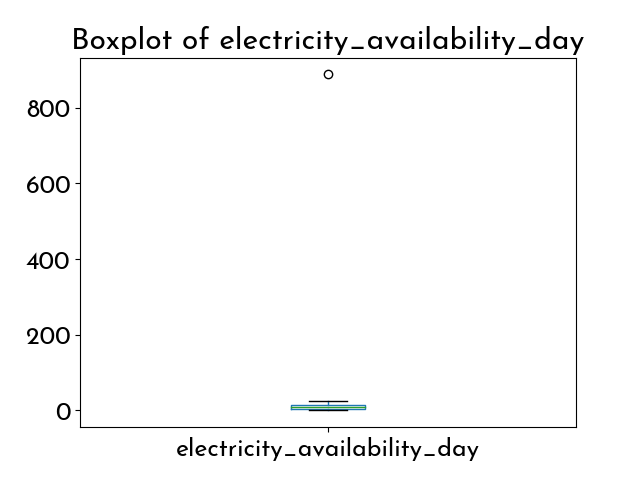
\includegraphics[scale=0.5]{/Users/chaix/Hedera/GIT/XLSform2PDF/output/svf/plots/graph_electricity_availability_day.png}
\end{figure}
\paragraph{For the last 7 days, how many hours of electricity were available each evening (on average), from 06:00pm to 10:00pm, from the electricity\_source\_label?}
\ \\ {\small If client is not sure, please ask for an estimation. One evening (6pm to 10pm) has 4 hours. If respondent has no idea, type 888 for 'I don't know'.}
\  \\Variable name: \texttt{electricity\_availability\_evening}\hfill\colorbox{red}{\small{\textcolor{white}{required}}}\\
 Type: integer\\
\\Total number of answers: 124 (50.6\%)
\\[0.2em] \begin{tabular}{p{4cm}|p{8cm}}
Minimum value &1.0 \\
\hline
\cellcolor{mygray} Maximum value & \cellcolor{mygray}4.0 \\
\hline
Variance &0.40519276160503537 \\
\hline
\cellcolor{mygray} Mean value & \cellcolor{mygray}3.596774193548387 \\
\hline
\end{tabular}
\begin{figure}[H]
\centering
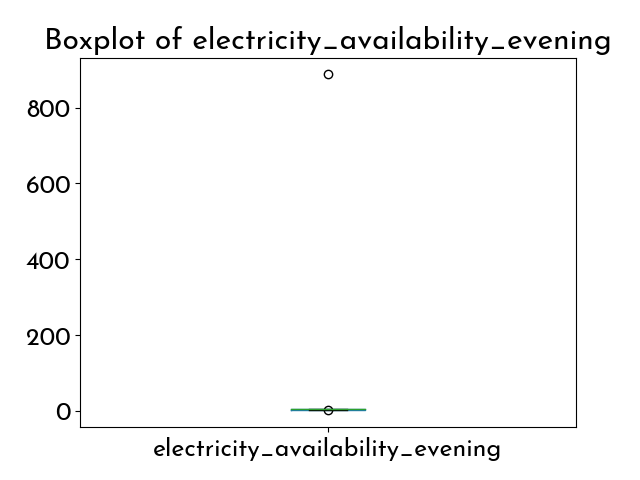
\includegraphics[scale=0.5]{/Users/chaix/Hedera/GIT/XLSform2PDF/output/svf/plots/graph_electricity_availability_evening.png}
\end{figure}
\paragraph{In the last 30 days, how many outages/blackouts of the electricity\_source\_label happen? (Number of interruptions)}
\ \\ {\small If client is not sure, please ask for an estimation. If respondent has no idea, type 888 for 'I don't know'.}
\  \\Variable name: \texttt{electricity\_reliability\_outages\_month\_number}\hfill\colorbox{red}{\small{\textcolor{white}{required}}}\\
 Type: integer\\
\\Total number of answers: 129 (52.7\%)
\\[0.2em] \begin{tabular}{p{4cm}|p{8cm}}
Minimum value &0.0 \\
\hline
\cellcolor{mygray} Maximum value & \cellcolor{mygray}30.0 \\
\hline
Variance &36.811894379844965 \\
\hline
\cellcolor{mygray} Mean value & \cellcolor{mygray}2.7829457364341086 \\
\hline
\end{tabular}
\begin{figure}[H]
\centering
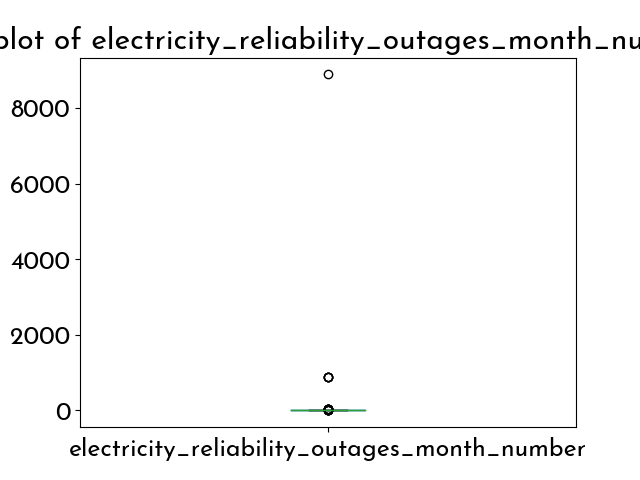
\includegraphics[scale=0.5]{/Users/chaix/Hedera/GIT/XLSform2PDF/output/svf/plots/graph_electricity_reliability_outages_month_number.png}
\end{figure}
\paragraph{How long was each outage/blackout, on average? }
\  \\Variable name: \texttt{electricity\_reliability\_outages\_length}\hfill\colorbox{red}{\small{\textcolor{white}{required}}}\\
 Type: single choice\\
\\Total number of answers: 62 (25.3\%)
\\[0.2em] \begin{tabular}{p{4cm}|p{8cm}|p{3cm}}
Choice code & Label & Answers \\
\hline
1 & Less than 1 hour& \cellcolor{color0}0 (0.0\%)\\
\cellcolor{mygray} 2 & \cellcolor{mygray}Between 1 hour and 1 day & \cellcolor{color0}0 (0.0\%)\\
3 & Between 1 and 3 days& \cellcolor{color0}0 (0.0\%)\\
\cellcolor{mygray} 4 & \cellcolor{mygray}More than 3 days & \cellcolor{color0}0 (0.0\%)\\
\end{tabular}
\paragraph{In the last 12 months, did you experienced voltage problems that damaged your appliances?}
\  \\Variable name: \texttt{electricity\_quality}\\
Type: single choice\\
\\Total number of answers: 120 (49.0\%)
\\[0.2em] \begin{tabular}{p{4cm}|p{8cm}|p{3cm}}
Choice code & Label & Answers \\
\hline
yes & Yes& \cellcolor{color0}20 (16.7\%)\\
\cellcolor{mygray} no & \cellcolor{mygray}No & \cellcolor{color4}100 (83.3\%)\\
\end{tabular}
\paragraph{Was there any bodily harm or accident related to your electricity supply in your household in the last 12 months?}
\  \\Variable name: \texttt{electricity\_injury\_list}\hfill\colorbox{red}{\small{\textcolor{white}{required}}}\\
 Type: multiple choice\\
\\Total number of answers: 134 (54.7\%)
\\[0.2em] \begin{tabular}{p{4cm}|p{8cm}|p{3cm}}
Choice code & Label & Answers \\
\hline
none & None& \cellcolor{color4}131 (97.8\%)\\
\cellcolor{mygray} burns & \cellcolor{mygray}Burns or electrocution & \cellcolor{color0}2 (1.5\%)\\
fire & Fire & \cellcolor{color0}0 (0.0\%)\\
\cellcolor{mygray} minor & \cellcolor{mygray}Other minor injury & \cellcolor{color0}1 (0.7\%)\\
permanent & Permanent damage, limb body injury& \cellcolor{color0}0 (0.0\%)\\
\cellcolor{mygray} death & \cellcolor{mygray}Death & \cellcolor{color0}0 (0.0\%)\\
\end{tabular}
\newpage\section{Cooking}
\paragraph{Can I see your stove / cooking area? Can I take a photo?}
\  \\Variable name: \texttt{image\_cooking\_stove}\\
Type: image\\
\paragraph{Which type of cookstove is primarily used in the household?}
\  \\Variable name: \texttt{cooking\_main\_stove}\hfill\colorbox{red}{\small{\textcolor{white}{required}}}\\
 Type: single choice\\
\\Total number of answers: 245 (100.0\%)
\\[0.2em] \begin{tabular}{p{4cm}|p{8cm}|p{3cm}}
Choice code & Label & Answers \\
\hline
none & None& \cellcolor{color0}2 (0.8\%)\\
\cellcolor{mygray} three\_stones & \cellcolor{mygray}Traditional three-stone fireplace & \cellcolor{color3}196 (80.0\%)\\
handmade & Simple clay stove that uses solid fuel& \cellcolor{color0}25 (10.2\%)\\
\cellcolor{mygray} manufactured\_solid & \cellcolor{mygray}Simple metal stove that uses solid fuel & \cellcolor{color0}13 (5.3\%)\\
improved\_cooking\_stove & Improved metal stove that uses solid fuel& \cellcolor{color0}9 (3.7\%)\\
\cellcolor{mygray} manufactured\_liquid & \cellcolor{mygray}Prefabricated stove that uses liquid fuel (e.g., kerosene, methanol, …) & \cellcolor{color0}0 (0.0\%)\\
lpg & LPG gas cooker& \cellcolor{color0}0 (0.0\%)\\
\cellcolor{mygray} biogas\_stove & \cellcolor{mygray}Biogas stove  & \cellcolor{color0}0 (0.0\%)\\
other & Other& \cellcolor{color0}0 (0.0\%)\\
\end{tabular}
\paragraph{Please specify:}
\  \\Variable name: \texttt{cooking\_main\_stove\_other}\hfill\colorbox{red}{\small{\textcolor{white}{required}}}\\
 Type: text\\
\\Total number of answers: 245 (100.0\%)
\\[0.2em]\paragraph{Which other cookstoves are used in the household?}
\ \\ {\small Select all that apply.}
\  \\Variable name: \texttt{cooking\_secondary\_solution}\hfill\colorbox{red}{\small{\textcolor{white}{required}}}\\
 Type: multiple choice\\
\\Total number of answers: 243 (99.2\%)
\\[0.2em] \begin{tabular}{p{4cm}|p{8cm}|p{3cm}}
Choice code & Label & Answers \\
\hline
none & None& \cellcolor{color3}190 (78.2\%)\\
\cellcolor{mygray} three\_stones & \cellcolor{mygray}Traditional three-stone fireplace & \cellcolor{color0}27 (11.1\%)\\
handmade & Simple clay stove that uses solid fuel& \cellcolor{color0}11 (4.5\%)\\
\cellcolor{mygray} manufactured\_solid & \cellcolor{mygray}Simple metal stove that uses solid fuel & \cellcolor{color0}9 (3.7\%)\\
improved\_cooking\_stove & Improved metal stove that uses solid fuel& \cellcolor{color0}6 (2.5\%)\\
\cellcolor{mygray} manufactured\_liquid & \cellcolor{mygray}Prefabricated stove that uses liquid fuel (e.g., kerosene, methanol, …) & \cellcolor{color0}0 (0.0\%)\\
lpg & LPG gas cooker& \cellcolor{color0}0 (0.0\%)\\
\cellcolor{mygray} biogas\_stove & \cellcolor{mygray}Biogas stove  & \cellcolor{color0}0 (0.0\%)\\
other & Other& \cellcolor{color0}0 (0.0\%)\\
\end{tabular}
\paragraph{Please specify:}
\  \\Variable name: \texttt{cooking\_secondary\_solution\_other}\\
Type: text\\
\\Total number of answers: 243 (99.2\%)
\\[0.2em]\paragraph{Why do you use more than one stove?}
\  \\Variable name: \texttt{cooking\_multiple\_stove\_reason}\\
Type: single choice\\
\\Total number of answers: 18 (7.3\%)
\\[0.2em] \begin{tabular}{p{4cm}|p{8cm}|p{3cm}}
Choice code & Label & Answers \\
\hline
1 & Tradition & \cellcolor{color0}2 (11.1\%)\\
\cellcolor{mygray} 2 & \cellcolor{mygray}To save on gas expenses & \cellcolor{color0}0 (0.0\%)\\
3 & Because of the taste of the meal& \cellcolor{color0}0 (0.0\%)\\
\cellcolor{mygray} 4 & \cellcolor{mygray}Lack of fuel for the primary stove & \cellcolor{color1}7 (38.9\%)\\
other & Other reason& \cellcolor{color2}9 (50.0\%)\\
\end{tabular}
\paragraph{Please specify:}
\  \\Variable name: \texttt{cooking\_multiple\_stove\_reason\_other}\\
Type: text\\
\\Total number of answers: 18 (7.3\%)
\\[0.2em]\begin{table}[H]
 \begin{tabular}{p{4cm}|p{8cm}}
Word & Number of occurrences  \\
\hline
\cellcolor{mygray}cook&\cellcolor{mygray}8\\
\hline
different&6\\
\hline
\cellcolor{mygray}food&\cellcolor{mygray}6\\
\hline
varieties&4\\
\hline
\cellcolor{mygray}less&\cellcolor{mygray}4\\
\hline
time&4\\
\hline
\cellcolor{mygray}sometimes&\cellcolor{mygray}2\\
\hline
cooking&1\\
\hline
\end{tabular}
\caption{\label{tab:table-name} Most used words for this answer}
\end{table}
\paragraph{How many times is food cooked in your household per day?}
\  \\Variable name: \texttt{cooking\_times\_per\_day}\hfill\colorbox{red}{\small{\textcolor{white}{required}}}\\
 Type: integer\\
\\Total number of answers: 243 (99.2\%)
\\[0.2em] \begin{tabular}{p{4cm}|p{8cm}}
Minimum value &1.0 \\
\hline
\cellcolor{mygray} Maximum value & \cellcolor{mygray}3.0 \\
\hline
Variance &0.2959221848110737 \\
\hline
\cellcolor{mygray} Mean value & \cellcolor{mygray}1.7325102880658436 \\
\hline
\end{tabular}
\begin{figure}[H]
\centering
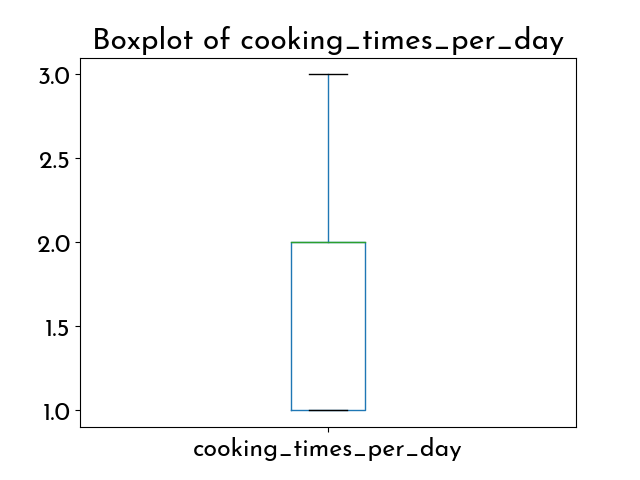
\includegraphics[scale=0.5]{/Users/chaix/Hedera/GIT/XLSform2PDF/output/svf/plots/graph_cooking_times_per_day.png}
\end{figure}
\paragraph{How much does your household spend on the LPG for the main cookstove in the last month/in a typical month when you use the stove? (Amount in Local Currency) }
\ \\ {\small Please enter the actual value spent, not the market value. If client is not sure, ask for an estimation or type 888, if client does not know at all. }
\  \\Variable name: \texttt{cooking\_lpg\_fuel\_price}\hfill\colorbox{red}{\small{\textcolor{white}{required}}}\\
 Type: integer\\
\\Total number of answers: 0 (0.0\%)
\\[0.2em]\paragraph{In which months is LPG available?}
\  \\Variable name: \texttt{cooking\_lpg\_fuel\_availability}\hfill\colorbox{red}{\small{\textcolor{white}{required}}}\\
 Type: multiple choice\\
\paragraph{Which solid fuels are used in the simple metal stove?}
\  \\Variable name: \texttt{cooking\_manufactured\_solid\_used\_fuels}\hfill\colorbox{red}{\small{\textcolor{white}{required}}}\\
 Type: multiple choice\\
\\Total number of answers: 13 (5.3\%)
\\[0.2em] \begin{tabular}{p{4cm}|p{8cm}|p{3cm}}
Choice code & Label & Answers \\
\hline
wood & Wood& \cellcolor{color3}9 (69.2\%)\\
\cellcolor{mygray} animal\_waste & \cellcolor{mygray}Animal Waste/Dung & \cellcolor{color0}0 (0.0\%)\\
crop\_residue & Crop Residue/Plant Biomass& \cellcolor{color0}0 (0.0\%)\\
\cellcolor{mygray} saw\_dust & \cellcolor{mygray}Saw Dust & \cellcolor{color0}0 (0.0\%)\\
biomass\_briquette & Biomass Briquette& \cellcolor{color0}0 (0.0\%)\\
\cellcolor{mygray} woodchips & \cellcolor{mygray}Processed Biomass (Pellets)/Woodchips & \cellcolor{color0}0 (0.0\%)\\
plastic & Garbage/Plastic& \cellcolor{color0}0 (0.0\%)\\
\cellcolor{mygray} charcoal & \cellcolor{mygray}Charcoal & \cellcolor{color1}4 (30.8\%)\\
other & Other Solid Fuels& \cellcolor{color0}0 (0.0\%)\\
\end{tabular}
\paragraph{Please specify any other solid fuel used on this stove}
\  \\Variable name: \texttt{cooking\_manufactured\_solid\_used\_fuels\_other}\\
Type: text\\
\\Total number of answers: 13 (5.3\%)
\\[0.2em]\paragraph{Which solid fuels are used in the three-stone fireplace/simple clay stove?}
\  \\Variable name: \texttt{cooking\_handmade\_used\_fuels}\hfill\colorbox{red}{\small{\textcolor{white}{required}}}\\
 Type: multiple choice\\
\\Total number of answers: 221 (90.2\%)
\\[0.2em] \begin{tabular}{p{4cm}|p{8cm}|p{3cm}}
Choice code & Label & Answers \\
\hline
wood & Wood& \cellcolor{color4}221 (100.0\%)\\
\cellcolor{mygray} animal\_waste & \cellcolor{mygray}Animal Waste/Dung & \cellcolor{color0}0 (0.0\%)\\
crop\_residue & Crop Residue/Plant Biomass& \cellcolor{color0}0 (0.0\%)\\
\cellcolor{mygray} saw\_dust & \cellcolor{mygray}Saw Dust & \cellcolor{color0}0 (0.0\%)\\
biomass\_briquette & Biomass Briquette& \cellcolor{color0}0 (0.0\%)\\
\cellcolor{mygray} woodchips & \cellcolor{mygray}Processed Biomass (Pellets)/Woodchips & \cellcolor{color0}0 (0.0\%)\\
plastic & Garbage/Plastic& \cellcolor{color0}2 (0.9\%)\\
\cellcolor{mygray} charcoal & \cellcolor{mygray}Charcoal & \cellcolor{color0}3 (1.4\%)\\
other & Other Solid Fuels& \cellcolor{color0}0 (0.0\%)\\
\end{tabular}
\paragraph{Please specify any other solid fuel used on this stove}
\  \\Variable name: \texttt{cooking\_handmade\_used\_fuels\_other}\\
Type: text\\
\\Total number of answers: 221 (90.2\%)
\\[0.2em]\paragraph{Which solid fuels are used in the improved metal stove?}
\  \\Variable name: \texttt{cooking\_improved\_cooking\_stove\_used\_fuels}\\
Type: multiple choice\\
\\Total number of answers: 9 (3.7\%)
\\[0.2em] \begin{tabular}{p{4cm}|p{8cm}|p{3cm}}
Choice code & Label & Answers \\
\hline
wood & Wood& \cellcolor{color4}9 (100.0\%)\\
\cellcolor{mygray} animal\_waste & \cellcolor{mygray}Animal Waste/Dung & \cellcolor{color0}0 (0.0\%)\\
crop\_residue & Crop Residue/Plant Biomass& \cellcolor{color0}0 (0.0\%)\\
\cellcolor{mygray} saw\_dust & \cellcolor{mygray}Saw Dust & \cellcolor{color0}0 (0.0\%)\\
biomass\_briquette & Biomass Briquette& \cellcolor{color0}0 (0.0\%)\\
\cellcolor{mygray} woodchips & \cellcolor{mygray}Processed Biomass (Pellets)/Woodchips & \cellcolor{color0}0 (0.0\%)\\
plastic & Garbage/Plastic& \cellcolor{color0}0 (0.0\%)\\
\cellcolor{mygray} charcoal & \cellcolor{mygray}Charcoal & \cellcolor{color0}0 (0.0\%)\\
other & Other Solid Fuels& \cellcolor{color0}0 (0.0\%)\\
\end{tabular}
\paragraph{Please specify any other solid fuel used on this stove}
\  \\Variable name: \texttt{cooking\_improved\_cooking\_stove\_used\_fuels\_other}\\
Type: text\\
\\Total number of answers: 9 (3.7\%)
\\[0.2em]\paragraph{How much does your household spend on gas for the main cookstove in the last month/in a typical month when you use the stove? (Amount in Local Currency) }
\ \\ {\small Please enter the actual value spent, not the market value. If client is not sure, ask for an estimation or type 888, if client does not know at all. }
\  \\Variable name: \texttt{cooking\_natural\_gas\_fuel\_price}\hfill\colorbox{red}{\small{\textcolor{white}{required}}}\\
 Type: integer\\
\\Total number of answers: 0 (0.0\%)
\\[0.2em]\paragraph{Which liquid fuels are used in the prefabricated stove?}
\  \\Variable name: \texttt{cooking\_manufactured\_liquid\_used\_fuels}\hfill\colorbox{red}{\small{\textcolor{white}{required}}}\\
 Type: multiple choice\\
\paragraph{Please specify any other liquid fuel used on this stove}
\  \\Variable name: \texttt{cooking\_manufactured\_solid\_used\_fuels\_other}\\
Type: text\\
\\Total number of answers: 0 (0.0\%)
\\[0.2em]\paragraph{How much does your household spend on electricity for the main cookstove in the last month/in a typical month when you use the stove? (Amount in Local Currency) }
\ \\ {\small Please enter the actual value spent, not the market value. If client is not sure, ask for an estimation or type 888, if client does not know at all. }
\  \\Variable name: \texttt{cooking\_electric\_fuel\_price}\hfill\colorbox{red}{\small{\textcolor{white}{required}}}\\
 Type: integer\\
\\Total number of answers: 0 (0.0\%)
\\[0.2em]\paragraph{In which months is electricity available?}
\  \\Variable name: \texttt{cooking\_electric\_fuel\_availability}\hfill\colorbox{red}{\small{\textcolor{white}{required}}}\\
 Type: multiple choice\\
\paragraph{In which months is biogas available?}
\  \\Variable name: \texttt{cooking\_biogas\_fuel\_availability}\hfill\colorbox{red}{\small{\textcolor{white}{required}}}\\
 Type: multiple choice\\
\paragraph{In which months is there sufficient solar energy to use the solar cooker?}
\  \\Variable name: \texttt{cooking\_solar\_fuel\_availability}\hfill\colorbox{red}{\small{\textcolor{white}{required}}}\\
 Type: multiple choice\\
\paragraph{How much does your household spend on kerosene for the main stove in the last month/in a typical month when you use the stove? (Amount in Local Currency) }
\ \\ {\small Please enter the actual value spent, not the market value. If client is not sure, ask for an estimation or type 888, if client does not at all. }
\  \\Variable name: \texttt{cooking\_fuel\_kerosene\_price}\hfill\colorbox{red}{\small{\textcolor{white}{required}}}\\
 Type: integer\\
\\Total number of answers: 0 (0.0\%)
\\[0.2em]\paragraph{In which months is kerosene available?}
\  \\Variable name: \texttt{cooking\_fuel\_kerosene\_availability}\hfill\colorbox{red}{\small{\textcolor{white}{required}}}\\
 Type: multiple choice\\
\paragraph{How much  does your household spend on ethanol/alcohol for the main stove in the last month/in a typical month when you use the stove? (Amount in Local Currency) }
\ \\ {\small Please enter the actual value spent, not the market value. If client is not sure, ask for an estimation or type 888, if client does not at all. }
\  \\Variable name: \texttt{cooking\_fuel\_ethanol\_price}\hfill\colorbox{red}{\small{\textcolor{white}{required}}}\\
 Type: integer\\
\\Total number of answers: 0 (0.0\%)
\\[0.2em]\paragraph{In which months is ethanol available?}
\  \\Variable name: \texttt{cooking\_fuel\_ethanol\_availability}\hfill\colorbox{red}{\small{\textcolor{white}{required}}}\\
 Type: multiple choice\\
\paragraph{How much does your household spend on methanol for the main stove in the last month/in a typical month when you use the stove? (Amount in Local Currency) }
\ \\ {\small Please enter the actual value spent, not the market value. If client is not sure, ask for an estimation or type 888, if client does not at all. }
\  \\Variable name: \texttt{cooking\_fuel\_methanol\_price}\hfill\colorbox{red}{\small{\textcolor{white}{required}}}\\
 Type: integer\\
\\Total number of answers: 0 (0.0\%)
\\[0.2em]\paragraph{In which months is methanol available?}
\  \\Variable name: \texttt{cooking\_fuel\_methanol\_availability}\hfill\colorbox{red}{\small{\textcolor{white}{required}}}\\
 Type: multiple choice\\
\paragraph{How much  does your household spend on oil for the main stove in the last month/in a typical month when you use the stove? (Amount in Local Currency) }
\ \\ {\small Please enter the actual value spent, not the market value. If client is not sure, ask for an estimation or type 888, if client does not at all. }
\  \\Variable name: \texttt{cooking\_fuel\_oil\_price}\hfill\colorbox{red}{\small{\textcolor{white}{required}}}\\
 Type: integer\\
\\Total number of answers: 0 (0.0\%)
\\[0.2em]\paragraph{In which months is oil available?}
\  \\Variable name: \texttt{cooking\_fuel\_oil\_availability}\hfill\colorbox{red}{\small{\textcolor{white}{required}}}\\
 Type: multiple choice\\
\paragraph{How much does your household spend on coal or lignite for the main stove in the last month/in a typical month when you use the stove? (Amount in Local Currency) }
\ \\ {\small Please enter the actual value spent, not the market value. If client is not sure, ask for an estimation or type 888, if client does not at all. }
\  \\Variable name: \texttt{cooking\_fuel\_coal\_price}\hfill\colorbox{red}{\small{\textcolor{white}{required}}}\\
 Type: integer\\
\\Total number of answers: 0 (0.0\%)
\\[0.2em]\paragraph{In which months is coal available?}
\  \\Variable name: \texttt{cooking\_fuel\_coal\_availability}\hfill\colorbox{red}{\small{\textcolor{white}{required}}}\\
 Type: multiple choice\\
\paragraph{How much  does your household spend on charcoal for this stove in the last month/in a typical month when you use the stove? (Amount in Local Currency) }
\ \\ {\small Please enter the actual value spent, not the market value. If client is not sure, ask for an estimation or type 888, if client does not at all. }
\  \\Variable name: \texttt{cooking\_fuel\_charcoal\_price}\hfill\colorbox{red}{\small{\textcolor{white}{required}}}\\
 Type: integer\\
\\Total number of answers: 5 (2.0\%)
\\[0.2em] \begin{tabular}{p{4cm}|p{8cm}}
Minimum value &2000.0 \\
\hline
\cellcolor{mygray} Maximum value & \cellcolor{mygray}8000.0 \\
\hline
Variance &7250000.0 \\
\hline
\cellcolor{mygray} Mean value & \cellcolor{mygray}5500.0 \\
\hline
\end{tabular}
\begin{figure}[H]
\centering
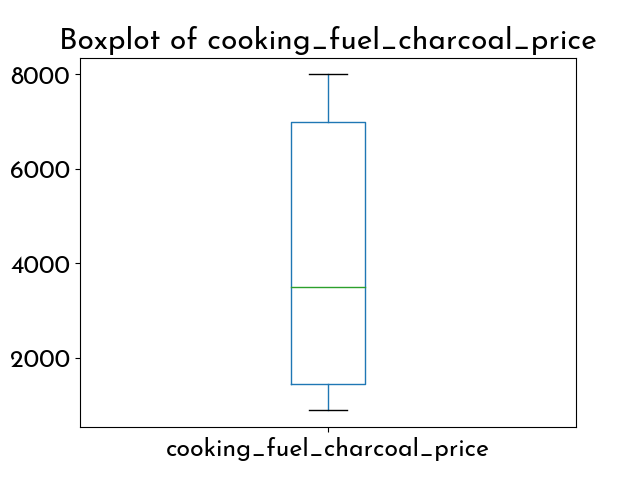
\includegraphics[scale=0.5]{/Users/chaix/Hedera/GIT/XLSform2PDF/output/svf/plots/graph_cooking_fuel_charcoal_price.png}
\end{figure}
\paragraph{In which months is charcoal available?}
\  \\Variable name: \texttt{cooking\_fuel\_charcoal\_availability}\hfill\colorbox{red}{\small{\textcolor{white}{required}}}\\
 Type: multiple choice\\
\\Total number of answers: 7 (2.9\%)
\\[0.2em] \begin{tabular}{p{4cm}|p{8cm}|p{3cm}}
Choice code & Label & Answers \\
\hline
all & Every month& \cellcolor{color1}2 (28.6\%)\\
\cellcolor{mygray} jan & \cellcolor{mygray}January & \cellcolor{color2}4 (57.1\%)\\
feb & February& \cellcolor{color2}3 (42.9\%)\\
\cellcolor{mygray} mar & \cellcolor{mygray}March & \cellcolor{color0}1 (14.3\%)\\
aor & April& \cellcolor{color0}0 (0.0\%)\\
\cellcolor{mygray} may & \cellcolor{mygray}May & \cellcolor{color0}1 (14.3\%)\\
jun & June& \cellcolor{color3}5 (71.4\%)\\
\cellcolor{mygray} jul & \cellcolor{mygray}July & \cellcolor{color3}5 (71.4\%)\\
aug & August& \cellcolor{color3}5 (71.4\%)\\
\cellcolor{mygray} sep  & \cellcolor{mygray}September & \cellcolor{color0}0 (0.0\%)\\
oct  & October& \cellcolor{color0}0 (0.0\%)\\
\cellcolor{mygray} nov & \cellcolor{mygray}November & \cellcolor{color1}2 (28.6\%)\\
dec  & December& \cellcolor{color0}0 (0.0\%)\\
\cellcolor{mygray} na & \cellcolor{mygray}Does not apply & \cellcolor{color0}1 (14.3\%)\\
\end{tabular}
\paragraph{How do you get your wood for cooking?}
\  \\Variable name: \texttt{cooking\_fuel\_wood\_source}\hfill\colorbox{red}{\small{\textcolor{white}{required}}}\\
 Type: multiple choice\\
\\Total number of answers: 239 (97.6\%)
\\[0.2em] \begin{tabular}{p{4cm}|p{8cm}|p{3cm}}
Choice code & Label & Answers \\
\hline
vendor & Buy from a vendor & \cellcolor{color1}56 (23.4\%)\\
\cellcolor{mygray} family & \cellcolor{mygray}From the family farm/ property  & \cellcolor{color0}24 (10.0\%)\\
collect & Collect in other places& \cellcolor{color4}196 (82.0\%)\\
\cellcolor{mygray} other & \cellcolor{mygray}Other  & \cellcolor{color0}1 (0.4\%)\\
\end{tabular}
\paragraph{How much  does your household spend on wood for the main stove in the last month/in a typical month when you use the stove? (Amount in Local Currency) }
\ \\ {\small Please enter the actual value spent, not the market value. If client is not sure, ask for an estimation or type 888, if client does not at all. }
\  \\Variable name: \texttt{cooking\_fuel\_wood\_price}\hfill\colorbox{red}{\small{\textcolor{white}{required}}}\\
 Type: integer\\
\\Total number of answers: 52 (21.2\%)
\\[0.2em] \begin{tabular}{p{4cm}|p{8cm}}
Minimum value &500.0 \\
\hline
\cellcolor{mygray} Maximum value & \cellcolor{mygray}20000.0 \\
\hline
Variance &27268005.279034693 \\
\hline
\cellcolor{mygray} Mean value & \cellcolor{mygray}8105.7692307692305 \\
\hline
\end{tabular}
\begin{figure}[H]
\centering
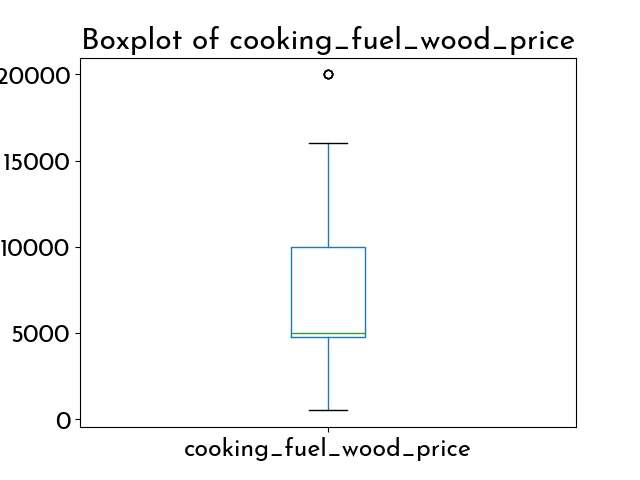
\includegraphics[scale=0.5]{/Users/chaix/Hedera/GIT/XLSform2PDF/output/svf/plots/graph_cooking_fuel_wood_price.png}
\end{figure}
\paragraph{In which months is wood for the cookstove available?}
\  \\Variable name: \texttt{cooking\_fuel\_wood\_availability}\hfill\colorbox{red}{\small{\textcolor{white}{required}}}\\
 Type: multiple choice\\
\\Total number of answers: 239 (97.6\%)
\\[0.2em] \begin{tabular}{p{4cm}|p{8cm}|p{3cm}}
Choice code & Label & Answers \\
\hline
all & Every month& \cellcolor{color1}48 (20.1\%)\\
\cellcolor{mygray} jan & \cellcolor{mygray}January & \cellcolor{color1}50 (20.9\%)\\
feb & February& \cellcolor{color1}56 (23.4\%)\\
\cellcolor{mygray} mar & \cellcolor{mygray}March & \cellcolor{color0}9 (3.8\%)\\
aor & April& \cellcolor{color0}0 (0.0\%)\\
\cellcolor{mygray} may & \cellcolor{mygray}May & \cellcolor{color0}16 (6.7\%)\\
jun & June& \cellcolor{color3}181 (75.7\%)\\
\cellcolor{mygray} jul & \cellcolor{mygray}July & \cellcolor{color3}188 (78.7\%)\\
aug & August& \cellcolor{color3}186 (77.8\%)\\
\cellcolor{mygray} sep  & \cellcolor{mygray}September & \cellcolor{color0}0 (0.0\%)\\
oct  & October& \cellcolor{color0}0 (0.0\%)\\
\cellcolor{mygray} nov & \cellcolor{mygray}November & \cellcolor{color0}45 (18.8\%)\\
dec  & December& \cellcolor{color0}0 (0.0\%)\\
\cellcolor{mygray} na & \cellcolor{mygray}Does not apply & \cellcolor{color0}3 (1.3\%)\\
\end{tabular}
\paragraph{How do you get your animal waste or dung for cooking?}
\  \\Variable name: \texttt{cooking\_fuel\_animal\_waste\_source}\hfill\colorbox{red}{\small{\textcolor{white}{required}}}\\
 Type: multiple choice\\
\paragraph{How much  does your household spend on animal waste/dung for this stove in the last month/in a typical month when you use the stove? (Amount in Local Currency) }
\ \\ {\small Please enter the actual value spent, not the market value. If client is not sure, ask for an estimation or type 888, if client does not at all. }
\  \\Variable name: \texttt{cooking\_fuel\_animal\_waste\_price}\hfill\colorbox{red}{\small{\textcolor{white}{required}}}\\
 Type: integer\\
\\Total number of answers: 0 (0.0\%)
\\[0.2em]\paragraph{In which months is animal waste for the cookstove available?}
\  \\Variable name: \texttt{cooking\_fuel\_animal\_waste\_availability}\hfill\colorbox{red}{\small{\textcolor{white}{required}}}\\
 Type: multiple choice\\
\paragraph{How do you get the crop residue for cooking?}
\  \\Variable name: \texttt{cooking\_fuel\_crop\_residue\_source}\hfill\colorbox{red}{\small{\textcolor{white}{required}}}\\
 Type: multiple choice\\
\paragraph{How much  does your household spend on the Crop Residue/Plant Biomass for this stove in the last month/in a typical month when you use the stove? (Amount in Local Currency) }
\ \\ {\small Please enter the actual value spent, not the market value. If client is not sure, ask for an estimation or type 888, if client does not at all. }
\  \\Variable name: \texttt{cooking\_fuel\_crop\_residue\_price}\hfill\colorbox{red}{\small{\textcolor{white}{required}}}\\
 Type: integer\\
\\Total number of answers: 0 (0.0\%)
\\[0.2em]\paragraph{In which months are plan biomass/crop residue for the cookstove available?}
\  \\Variable name: \texttt{cooking\_fuel\_crop\_residue\_availability}\hfill\colorbox{red}{\small{\textcolor{white}{required}}}\\
 Type: multiple choice\\
\paragraph{How do you get the saw dust for cooking?}
\  \\Variable name: \texttt{cooking\_fuel\_saw\_dust\_source}\hfill\colorbox{red}{\small{\textcolor{white}{required}}}\\
 Type: multiple choice\\
\paragraph{How much  does your household spend on saw dust for this stove in the last month/in a typical month when you use the stove? (Amount in Local Currency) }
\ \\ {\small Please enter the actual value spent, not the market value. If client is not sure, ask for an estimation or type 888, if client does not at all. }
\  \\Variable name: \texttt{cooking\_fuel\_saw\_dust\_price}\hfill\colorbox{red}{\small{\textcolor{white}{required}}}\\
 Type: integer\\
\\Total number of answers: 0 (0.0\%)
\\[0.2em]\paragraph{In which months is saw dust for the cookstove available?}
\  \\Variable name: \texttt{cooking\_fuel\_saw\_dust\_availability}\hfill\colorbox{red}{\small{\textcolor{white}{required}}}\\
 Type: multiple choice\\
\paragraph{How much  does your household spend on coal briquettes for this stove in the last month/in a typical month when you use the stove? (Amount in Local Currency) }
\ \\ {\small Please enter the actual value spent, not the market value. If client is not sure, ask for an estimation or type 888, if client does not at all. }
\  \\Variable name: \texttt{cooking\_fuel\_coal\_briquette\_price}\hfill\colorbox{red}{\small{\textcolor{white}{required}}}\\
 Type: integer\\
\\Total number of answers: 0 (0.0\%)
\\[0.2em]\paragraph{In which months are coal briquettes available?}
\  \\Variable name: \texttt{cooking\_fuel\_plant\_biomass\_availability}\hfill\colorbox{red}{\small{\textcolor{white}{required}}}\\
 Type: multiple choice\\
\paragraph{How much  does your household spend on biomass briquette for this stove in the last month/in a typical month when you use the stove? (Amount in Local Currency) }
\ \\ {\small Please enter the actual value spent, not the market value. If client is not sure, ask for an estimation or type 888, if client does not at all. }
\  \\Variable name: \texttt{cooking\_fuel\_biomass\_briquette\_price}\hfill\colorbox{red}{\small{\textcolor{white}{required}}}\\
 Type: integer\\
\\Total number of answers: 0 (0.0\%)
\\[0.2em]\paragraph{In which months are biomass briquettes available?}
\  \\Variable name: \texttt{cooking\_fuel\_biomass\_briquette\_availability}\hfill\colorbox{red}{\small{\textcolor{white}{required}}}\\
 Type: multiple choice\\
\paragraph{How much  does your household spend on Processed Biomass (Pellets)/Woodchips for this stove in the last month/in a typical month when you use the stove? (Amount in Local Currency) }
\ \\ {\small Please enter the actual value spent, not the market value. If client is not sure, ask for an estimation or type 888, if client does not at all. }
\  \\Variable name: \texttt{cooking\_fuel\_woodchips\_price}\hfill\colorbox{red}{\small{\textcolor{white}{required}}}\\
 Type: integer\\
\\Total number of answers: 0 (0.0\%)
\\[0.2em]\paragraph{In which months are pellets/woodchips available?}
\  \\Variable name: \texttt{cooking\_fuel\_woodchips\_availability}\hfill\colorbox{red}{\small{\textcolor{white}{required}}}\\
 Type: multiple choice\\
\paragraph{How much  does your household spend on the garbage/plastic for this stove in the last month/in a typical month when you use the stove? (Amount in Local Currency) }
\ \\ {\small Please enter the actual value spent, not the market value. If client is not sure, ask for an estimation or type 888, if client does not at all. }
\  \\Variable name: \texttt{cooking\_fuel\_plastic\_price}\hfill\colorbox{red}{\small{\textcolor{white}{required}}}\\
 Type: integer\\
\\Total number of answers: 2 (0.8\%)
\\[0.2em] \begin{tabular}{p{4cm}|p{8cm}}
Minimum value &5000.0 \\
\hline
\cellcolor{mygray} Maximum value & \cellcolor{mygray}5000.0 \\
\hline
Variance &0.0 \\
\hline
\cellcolor{mygray} Mean value & \cellcolor{mygray}5000.0 \\
\hline
\end{tabular}
\begin{figure}[H]
\centering
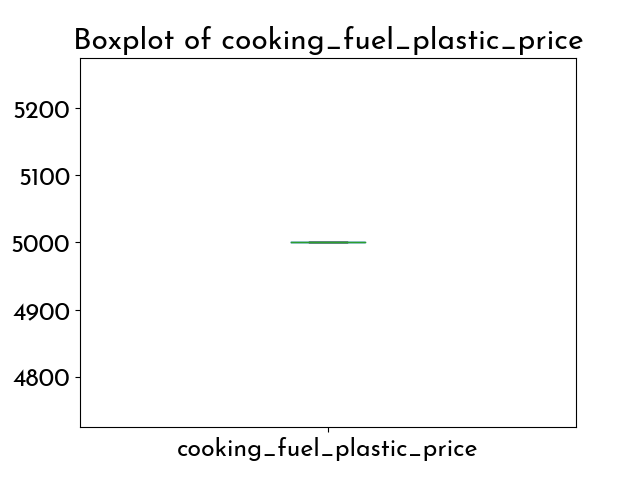
\includegraphics[scale=0.5]{/Users/chaix/Hedera/GIT/XLSform2PDF/output/svf/plots/graph_cooking_fuel_plastic_price.png}
\end{figure}
\paragraph{In which months is plastic/garbage for the cookstove available?}
\  \\Variable name: \texttt{cooking\_fuel\_plastic\_availability}\hfill\colorbox{red}{\small{\textcolor{white}{required}}}\\
 Type: multiple choice\\
\\Total number of answers: 2 (0.8\%)
\\[0.2em] \begin{tabular}{p{4cm}|p{8cm}|p{3cm}}
Choice code & Label & Answers \\
\hline
all & Every month& \cellcolor{color4}2 (100.0\%)\\
\cellcolor{mygray} jan & \cellcolor{mygray}January & \cellcolor{color0}0 (0.0\%)\\
feb & February& \cellcolor{color0}0 (0.0\%)\\
\cellcolor{mygray} mar & \cellcolor{mygray}March & \cellcolor{color0}0 (0.0\%)\\
aor & April& \cellcolor{color0}0 (0.0\%)\\
\cellcolor{mygray} may & \cellcolor{mygray}May & \cellcolor{color0}0 (0.0\%)\\
jun & June& \cellcolor{color0}0 (0.0\%)\\
\cellcolor{mygray} jul & \cellcolor{mygray}July & \cellcolor{color0}0 (0.0\%)\\
aug & August& \cellcolor{color0}0 (0.0\%)\\
\cellcolor{mygray} sep  & \cellcolor{mygray}September & \cellcolor{color0}0 (0.0\%)\\
oct  & October& \cellcolor{color0}0 (0.0\%)\\
\cellcolor{mygray} nov & \cellcolor{mygray}November & \cellcolor{color0}0 (0.0\%)\\
dec  & December& \cellcolor{color0}0 (0.0\%)\\
\cellcolor{mygray} na & \cellcolor{mygray}Does not apply & \cellcolor{color0}0 (0.0\%)\\
\end{tabular}
\paragraph{Where do members of your household normally cook with the cookstove? }
\  \\Variable name: \texttt{cookstove\_locality}\hfill\colorbox{red}{\small{\textcolor{white}{required}}}\\
 Type: single choice\\
\\Total number of answers: 243 (99.2\%)
\\[0.2em] \begin{tabular}{p{4cm}|p{8cm}|p{3cm}}
Choice code & Label & Answers \\
\hline
not\_sleeping & In dwelling, NOT in sleeping area& \cellcolor{color0}48 (19.8\%)\\
\cellcolor{mygray} sleeping & \cellcolor{mygray}In dwelling, in a sleeping area & \cellcolor{color0}7 (2.9\%)\\
separate\_dwelling & In a separate dwelling& \cellcolor{color3}154 (63.4\%)\\
\cellcolor{mygray} veranda & \cellcolor{mygray}In a veranda (roofed platform with at least two open sides)  & \cellcolor{color0}0 (0.0\%)\\
outdoors & Outdoors& \cellcolor{color0}33 (13.6\%)\\
\cellcolor{mygray} other & \cellcolor{mygray}Other & \cellcolor{color0}1 (0.4\%)\\
\end{tabular}
\paragraph{Please specify:}
\  \\Variable name: \texttt{cookstove\_locality\_other}\\
Type: text\\
\\Total number of answers: 243 (99.2\%)
\\[0.2em]\begin{table}[H]
 \begin{tabular}{p{4cm}|p{8cm}}
Word & Number of occurrences  \\
\hline
\cellcolor{mygray}old&\cellcolor{mygray}1\\
\hline
woman&1\\
\hline
\cellcolor{mygray}young&\cellcolor{mygray}1\\
\hline
lady&1\\
\hline
\cellcolor{mygray}cooks&\cellcolor{mygray}1\\
\hline
brings&1\\
\hline
\cellcolor{mygray}food&\cellcolor{mygray}1\\
\hline
everyday&1\\
\hline
\end{tabular}
\caption{\label{tab:table-name} Most used words for this answer}
\end{table}
\paragraph{Do members of your household usually use a chimney, hood or other exhaust system while using the stove? }
\  \\Variable name: \texttt{cookstove\_locality\_exhaust\_system}\hfill\colorbox{red}{\small{\textcolor{white}{required}}}\\
 Type: single choice\\
\\Total number of answers: 210 (85.7\%)
\\[0.2em] \begin{tabular}{p{4cm}|p{8cm}|p{3cm}}
Choice code & Label & Answers \\
\hline
yes & Yes& \cellcolor{color1}73 (34.8\%)\\
\cellcolor{mygray} no & \cellcolor{mygray}No & \cellcolor{color3}137 (65.2\%)\\
\end{tabular}
\paragraph{In the last 12 months, did you or anyone in your  households experience any injury or accidents while cooking?}
\  \\Variable name: \texttt{cooking\_injuries}\hfill\colorbox{red}{\small{\textcolor{white}{required}}}\\
 Type: multiple choice\\
\\Total number of answers: 243 (99.2\%)
\\[0.2em] \begin{tabular}{p{4cm}|p{8cm}|p{3cm}}
Choice code & Label & Answers \\
\hline
none & None& \cellcolor{color3}177 (72.8\%)\\
\cellcolor{mygray} minor & \cellcolor{mygray}Minor injury & \cellcolor{color0}48 (19.8\%)\\
death & Death & \cellcolor{color0}0 (0.0\%)\\
\cellcolor{mygray} permanent & \cellcolor{mygray}Permanent physical damage to any person in the household & \cellcolor{color0}1 (0.4\%)\\
burns & Burns/fire/poisoning& \cellcolor{color0}5 (2.1\%)\\
\cellcolor{mygray} respiratory & \cellcolor{mygray}Severe cough/respiratory problem & \cellcolor{color0}10 (4.1\%)\\
fire & Fire with no injury& \cellcolor{color0}6 (2.5\%)\\
\cellcolor{mygray} other & \cellcolor{mygray}Other major injury & \cellcolor{color0}0 (0.0\%)\\
\end{tabular}
\paragraph{Please specify:}
\  \\Variable name: \texttt{cooking\_injuries\_other}\\
Type: text\\
\\Total number of answers: 243 (99.2\%)
\\[0.2em]\paragraph{In the last 7 days, how many minutes per day (on average) did household members spend on gathering, collecting or purchasing the main fuel for the main cookstove, including travel time? }
\ \\ {\small Please answer in minutes per day. Type 888 if client does not know. }
\  \\Variable name: \texttt{cooking\_fuel\_collecting\_time}\hfill\colorbox{red}{\small{\textcolor{white}{required}}}\\
 Type: decimal\\
\newpage\section{Water, Sanitation, and Hygiene (WASH)}
\paragraph{What is the main source of drinking water for members of your household? }
\  \\Variable name: \texttt{water\_main\_source\_drinking}\hfill\colorbox{red}{\small{\textcolor{white}{required}}}\\
 Type: single choice\\
\\Total number of answers: 245 (100.0\%)
\\[0.2em] \begin{tabular}{p{4cm}|p{8cm}|p{3cm}}
Choice code & Label & Answers \\
\hline
none & None& \cellcolor{color0}1 (0.4\%)\\
\cellcolor{mygray} surface & \cellcolor{mygray}Surface water (river, stream, dam, lake, pond, canal, irrigation channel) & \cellcolor{color2}112 (45.7\%)\\
rainwater & Rainwater collection & \cellcolor{color2}115 (46.9\%)\\
\cellcolor{mygray} piped\_house & \cellcolor{mygray}Piped Water - Piped into house & \cellcolor{color0}0 (0.0\%)\\
piped\_yard & Piped Water - Piped into compound, yard, or plot& \cellcolor{color0}0 (0.0\%)\\
\cellcolor{mygray} piped\_nb & \cellcolor{mygray}Piped Water - Piped to neighbour  & \cellcolor{color0}0 (0.0\%)\\
piped\_tap & Piped Water - Public tap / standpipe & \cellcolor{color0}4 (1.6\%)\\
\cellcolor{mygray} piped\_borehole & \cellcolor{mygray}Piped Water - Borehole or tubewell  & \cellcolor{color0}0 (0.0\%)\\
dug\_covered & Dug well  - Covered, lined, and protected well & \cellcolor{color0}0 (0.0\%)\\
\cellcolor{mygray} dug\_uncovered & \cellcolor{mygray}Dug well  - Unprotected/uncovered/unlined well  & \cellcolor{color0}0 (0.0\%)\\
spring\_protected & Spring - Protected by spring box made of brick/concrete& \cellcolor{color0}0 (0.0\%)\\
\cellcolor{mygray} spring\_unprotected & \cellcolor{mygray}Spring - Unprotected  & \cellcolor{color0}0 (0.0\%)\\
delivered\_truck & Delivered water  - Tanker-truck & \cellcolor{color0}2 (0.8\%)\\
\cellcolor{mygray} delivered\_car & \cellcolor{mygray}Delivered water - Cart with small tank / drum & \cellcolor{color0}0 (0.0\%)\\
kiosk & Water kiosk& \cellcolor{color0}0 (0.0\%)\\
\cellcolor{mygray} packaged\_bottle & \cellcolor{mygray}Packaged - Bottled water & \cellcolor{color0}0 (0.0\%)\\
packaged\_sachet & Packaged - Sachet water & \cellcolor{color0}0 (0.0\%)\\
\cellcolor{mygray} other & \cellcolor{mygray}Other  & \cellcolor{color0}11 (4.5\%)\\
\end{tabular}
\paragraph{Please, specify what is your main source of drinking water}
\  \\Variable name: \texttt{water\_main\_source\_drinking\_other}\\
Type: text\\
\\Total number of answers: 245 (100.0\%)
\\[0.2em]\begin{table}[H]
 \begin{tabular}{p{4cm}|p{8cm}}
Word & Number of occurrences  \\
\hline
\cellcolor{mygray}water&\cellcolor{mygray}13\\
\hline
tap&6\\
\hline
\cellcolor{mygray}bring&\cellcolor{mygray}5\\
\hline
go&4\\
\hline
\cellcolor{mygray}pay&\cellcolor{mygray}4\\
\hline
buy&3\\
\hline
\cellcolor{mygray}sell&\cellcolor{mygray}3\\
\hline
someone&3\\
\hline
\end{tabular}
\caption{\label{tab:table-name} Most used words for this answer}
\end{table}
\paragraph{What are other sources of drinking water for members of your household?}
\ \\ {\small Select all that apply. }
\  \\Variable name: \texttt{water\_other\_source\_drinking}\hfill\colorbox{red}{\small{\textcolor{white}{required}}}\\
 Type: multiple choice\\
\\Total number of answers: 118 (48.2\%)
\\[0.2em] \begin{tabular}{p{4cm}|p{8cm}|p{3cm}}
Choice code & Label & Answers \\
\hline
none & None& \cellcolor{color0}13 (11.0\%)\\
\cellcolor{mygray} surface & \cellcolor{mygray}Surface water (river, stream, dam, lake, pond, canal, irrigation channel) & \cellcolor{color2}57 (48.3\%)\\
rainwater & Rainwater collection & \cellcolor{color2}54 (45.8\%)\\
\cellcolor{mygray} piped\_house & \cellcolor{mygray}Piped Water - Piped into house & \cellcolor{color0}0 (0.0\%)\\
piped\_yard & Piped Water - Piped into compound, yard, or plot& \cellcolor{color0}0 (0.0\%)\\
\cellcolor{mygray} piped\_nb & \cellcolor{mygray}Piped Water - Piped to neighbour  & \cellcolor{color0}0 (0.0\%)\\
piped\_tap & Piped Water - Public tap / standpipe & \cellcolor{color0}0 (0.0\%)\\
\cellcolor{mygray} piped\_borehole & \cellcolor{mygray}Piped Water - Borehole or tubewell  & \cellcolor{color0}0 (0.0\%)\\
dug\_covered & Dug well  - Covered, lined, and protected well & \cellcolor{color0}0 (0.0\%)\\
\cellcolor{mygray} dug\_uncovered & \cellcolor{mygray}Dug well  - Unprotected/uncovered/unlined well  & \cellcolor{color0}0 (0.0\%)\\
spring\_protected & Spring - Protected by spring box made of brick/concrete& \cellcolor{color0}0 (0.0\%)\\
\cellcolor{mygray} spring\_unprotected & \cellcolor{mygray}Spring - Unprotected  & \cellcolor{color0}0 (0.0\%)\\
delivered\_truck & Delivered water  - Tanker-truck & \cellcolor{color0}3 (2.5\%)\\
\cellcolor{mygray} delivered\_car & \cellcolor{mygray}Delivered water - Cart with small tank / drum & \cellcolor{color0}0 (0.0\%)\\
kiosk & Water kiosk& \cellcolor{color0}0 (0.0\%)\\
\cellcolor{mygray} packaged\_bottle & \cellcolor{mygray}Packaged - Bottled water & \cellcolor{color0}0 (0.0\%)\\
packaged\_sachet & Packaged - Sachet water & \cellcolor{color0}0 (0.0\%)\\
\cellcolor{mygray} other & \cellcolor{mygray}Other  & \cellcolor{color0}0 (0.0\%)\\
\end{tabular}
\paragraph{Please specify:}
\  \\Variable name: \texttt{water\_other\_source\_drinking\_other}\\
Type: text\\
\\Total number of answers: 118 (48.2\%)
\\[0.2em]\paragraph{What is the main source of water used by members of your household for other purposes, such as cooking and hand washing? }
\  \\Variable name: \texttt{water\_main\_source\_other\_purposes}\hfill\colorbox{red}{\small{\textcolor{white}{required}}}\\
 Type: single choice\\
\paragraph{Please, specify what is your main source for cooking and/or handwashing}
\  \\Variable name: \texttt{water\_main\_source\_other}\\
Type: text\\
\\Total number of answers: 0 (0.0\%)
\\[0.2em]\paragraph{Who manages the supply of drinking water?}
\  \\Variable name: \texttt{water\_main\_source\_supplier}\\
Type: text\\
\\Total number of answers: 0 (0.0\%)
\\[0.2em]\begin{table}[H]
 \begin{tabular}{p{4cm}|p{8cm}}
Word & Number of occurrences  \\
\hline
\cellcolor{mygray}government&\cellcolor{mygray}2\\
\hline
woman&2\\
\hline
\cellcolor{mygray}sogea&\cellcolor{mygray}1\\
\hline
go&1\\
\hline
\cellcolor{mygray}fetch&\cellcolor{mygray}1\\
\hline
water&1\\
\hline
\cellcolor{mygray}rwamagana&\cellcolor{mygray}1\\
\hline
district&1\\
\hline
\end{tabular}
\caption{\label{tab:table-name} Most used words for this answer}
\end{table}
\paragraph{Is the water supplied from your main source usually acceptable in terms of quality? }
\  \\Variable name: \texttt{water\_acceptability\_main\_source}\hfill\colorbox{red}{\small{\textcolor{white}{required}}}\\
 Type: single choice\\
\\Total number of answers: 245 (100.0\%)
\\[0.2em] \begin{tabular}{p{4cm}|p{8cm}|p{3cm}}
Choice code & Label & Answers \\
\hline
yes & Yes& \cellcolor{color0}17 (6.9\%)\\
\cellcolor{mygray} no & \cellcolor{mygray}No & \cellcolor{color4}228 (93.1\%)\\
\end{tabular}
\paragraph{If the water is unacceptable in terms of quality, what is the main problem with it?}
\  \\Variable name: \texttt{water\_acceptability\_main\_source\_reasons}\\
Type: single choice\\
\\Total number of answers: 228 (93.1\%)
\\[0.2em] \begin{tabular}{p{4cm}|p{8cm}|p{3cm}}
Choice code & Label & Answers \\
\hline
pollution & Pollution& \cellcolor{color4}183 (80.3\%)\\
\cellcolor{mygray} taste & \cellcolor{mygray}Taste & \cellcolor{color0}0 (0.0\%)\\
color & Color& \cellcolor{color0}0 (0.0\%)\\
\cellcolor{mygray} smell & \cellcolor{mygray}Smell & \cellcolor{color0}0 (0.0\%)\\
materials & It contains solid material& \cellcolor{color0}43 (18.9\%)\\
\cellcolor{mygray} other & \cellcolor{mygray}Other & \cellcolor{color0}2 (0.9\%)\\
\end{tabular}
\paragraph{Please specify:}
\  \\Variable name: \texttt{water\_acceptability\_main\_source\_reasons\_other}\\
Type: text\\
\\Total number of answers: 228 (93.1\%)
\\[0.2em]\begin{table}[H]
 \begin{tabular}{p{4cm}|p{8cm}}
Word & Number of occurrences  \\
\hline
\cellcolor{mygray}microorganism&\cellcolor{mygray}1\\
\hline
note&1\\
\hline
\cellcolor{mygray}shop&\cellcolor{mygray}1\\
\hline
information&1\\
\hline
\cellcolor{mygray}wash&\cellcolor{mygray}1\\
\hline
\end{tabular}
\caption{\label{tab:table-name} Most used words for this answer}
\end{table}
\paragraph{Is the piped water supply network you have access to large or small? Please select the most appropriate option.}
\  \\Variable name: \texttt{water\_accessibility\_piped\_network\_type}\\
Type: single choice\\
\\Total number of answers: 4 (1.6\%)
\\[0.2em] \begin{tabular}{p{4cm}|p{8cm}|p{3cm}}
Choice code & Label & Answers \\
\hline
1 & Large piped network managed by a utility & \cellcolor{color0}0 (0.0\%)\\
\cellcolor{mygray} 2 & \cellcolor{mygray}Small piped network managed by the community  & \cellcolor{color0}0 (0.0\%)\\
3 & Small piped network managed by the households& \cellcolor{color0}0 (0.0\%)\\
\end{tabular}
\paragraph{Where do you collect that water from? }
\  \\Variable name: \texttt{water\_accessibility\_source\_location}\hfill\colorbox{red}{\small{\textcolor{white}{required}}}\\
 Type: multiple choice\\
\\Total number of answers: 217 (88.6\%)
\\[0.2em] \begin{tabular}{p{4cm}|p{8cm}|p{3cm}}
Choice code & Label & Answers \\
\hline
house & In own house& \cellcolor{color1}78 (35.9\%)\\
\cellcolor{mygray} yard & \cellcolor{mygray}In own yard/plot & \cellcolor{color2}110 (50.7\%)\\
lake & From a lake& \cellcolor{color1}57 (26.3\%)\\
\cellcolor{mygray} river & \cellcolor{mygray}From a river & \cellcolor{color0}30 (13.8\%)\\
other & Elsewhere& \cellcolor{color0}24 (11.1\%)\\
\end{tabular}
\paragraph{Please specify:}
\  \\Variable name: \texttt{water\_accessibility\_source\_location\_other}\\
Type: text\\
\\Total number of answers: 217 (88.6\%)
\\[0.2em]\begin{table}[H]
 \begin{tabular}{p{4cm}|p{8cm}}
Word & Number of occurrences  \\
\hline
\cellcolor{mygray}water&\cellcolor{mygray}18\\
\hline
fetch&11\\
\hline
\cellcolor{mygray}lake&\cellcolor{mygray}10\\
\hline
go&8\\
\hline
\cellcolor{mygray}bring&\cellcolor{mygray}6\\
\hline
takes&5\\
\hline
\cellcolor{mygray}river&\cellcolor{mygray}4\\
\hline
far&4\\
\hline
\end{tabular}
\caption{\label{tab:table-name} Most used words for this answer}
\end{table}
\paragraph{Do members of the household collect water?}
\  \\Variable name: \texttt{water\_accessibility\_is\_collected}\hfill\colorbox{red}{\small{\textcolor{white}{required}}}\\
 Type: single choice\\
\\Total number of answers: 205 (83.7\%)
\\[0.2em] \begin{tabular}{p{4cm}|p{8cm}|p{3cm}}
Choice code & Label & Answers \\
\hline
yes & Yes& \cellcolor{color3}162 (79.0\%)\\
\cellcolor{mygray} no & \cellcolor{mygray}No & \cellcolor{color1}43 (21.0\%)\\
\end{tabular}
\paragraph{How long does it take to go to the water source, get water, and come back? [minutes]}
\ \\ {\small Record the total time taken for a single round trip, including queuing. }
\  \\Variable name: \texttt{water\_accessibility\_collection\_time}\hfill\colorbox{red}{\small{\textcolor{white}{required}}}\\
 Type: integer\\
\\Total number of answers: 161 (65.7\%)
\\[0.2em] \begin{tabular}{p{4cm}|p{8cm}}
Minimum value &0.0 \\
\hline
\cellcolor{mygray} Maximum value & \cellcolor{mygray}360.0 \\
\hline
Variance &4073.8975155279504 \\
\hline
\cellcolor{mygray} Mean value & \cellcolor{mygray}167.0496894409938 \\
\hline
\end{tabular}
\begin{figure}[H]
\centering
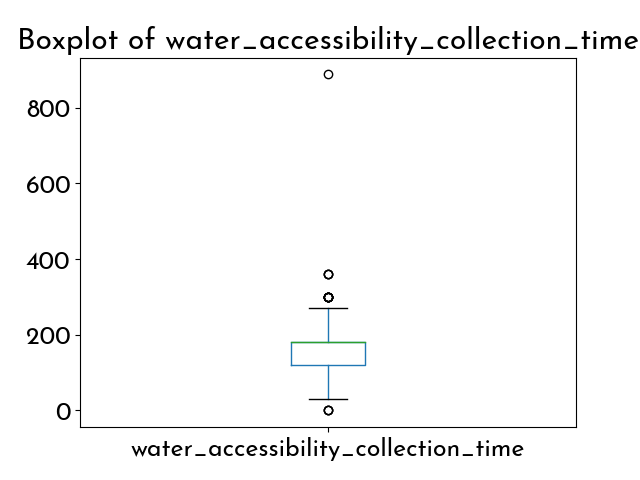
\includegraphics[scale=0.5]{/Users/chaix/Hedera/GIT/XLSform2PDF/output/svf/plots/graph_water_accessibility_collection_time.png}
\end{figure}
\paragraph{Who usually goes to this source to fetch water for your household? }
\  \\Variable name: \texttt{water\_accessibility\_collection\_who}\\
Type: multiple choice\\
\\Total number of answers: 161 (65.7\%)
\\[0.2em] \begin{tabular}{p{4cm}|p{8cm}|p{3cm}}
Choice code & Label & Answers \\
\hline
1 & Adult woman (16 years old and older) & \cellcolor{color3}108 (67.1\%)\\
\cellcolor{mygray} 2 & \cellcolor{mygray}Adult man (16 years old and older)  & \cellcolor{color3}120 (74.5\%)\\
3 & Children (under 16 years old) & \cellcolor{color1}56 (34.8\%)\\
\end{tabular}
\paragraph{How many trips in total did members of the household make on a typical day (e.g. yesterday) to fetch water?}
\  \\Variable name: \texttt{water\_accessibility\_collection\_trips}\\
Type: integer\\
\\Total number of answers: 160 (65.3\%)
\\[0.2em] \begin{tabular}{p{4cm}|p{8cm}}
Minimum value &0.0 \\
\hline
\cellcolor{mygray} Maximum value & \cellcolor{mygray}120.0 \\
\hline
Variance &88.24842767295597 \\
\hline
\cellcolor{mygray} Mean value & \cellcolor{mygray}2.125 \\
\hline
\end{tabular}
\begin{figure}[H]
\centering
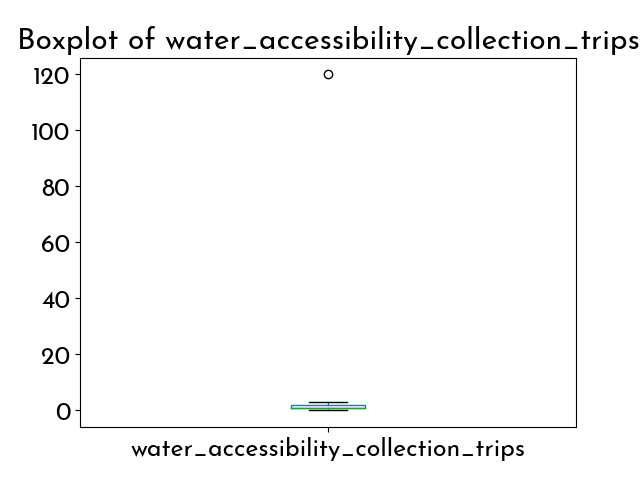
\includegraphics[scale=0.5]{/Users/chaix/Hedera/GIT/XLSform2PDF/output/svf/plots/graph_water_accessibility_collection_trips.png}
\end{figure}
\paragraph{Is there water scarcity over the year?}
\  \\Variable name: \texttt{water\_scarcity}\hfill\colorbox{red}{\small{\textcolor{white}{required}}}\\
 Type: single choice\\
\\Total number of answers: 202 (82.4\%)
\\[0.2em] \begin{tabular}{p{4cm}|p{8cm}|p{3cm}}
Choice code & Label & Answers \\
\hline
yes & Yes& \cellcolor{color2}102 (50.5\%)\\
\cellcolor{mygray} no & \cellcolor{mygray}No & \cellcolor{color2}100 (49.5\%)\\
\end{tabular}
\paragraph{In which months?}
\  \\Variable name: \texttt{water\_scarcity\_months}\hfill\colorbox{red}{\small{\textcolor{white}{required}}}\\
 Type: multiple choice\\
\\Total number of answers: 102 (41.6\%)
\\[0.2em] \begin{tabular}{p{4cm}|p{8cm}|p{3cm}}
Choice code & Label & Answers \\
\hline
all & Every month& \cellcolor{color0}0 (0.0\%)\\
\cellcolor{mygray} jan & \cellcolor{mygray}January & \cellcolor{color0}0 (0.0\%)\\
feb & February& \cellcolor{color0}0 (0.0\%)\\
\cellcolor{mygray} mar & \cellcolor{mygray}March & \cellcolor{color0}0 (0.0\%)\\
aor & April& \cellcolor{color0}1 (1.0\%)\\
\cellcolor{mygray} may & \cellcolor{mygray}May & \cellcolor{color0}10 (9.8\%)\\
jun & June& \cellcolor{color4}99 (97.1\%)\\
\cellcolor{mygray} jul & \cellcolor{mygray}July & \cellcolor{color4}100 (98.0\%)\\
aug & August& \cellcolor{color4}100 (98.0\%)\\
\cellcolor{mygray} sep  & \cellcolor{mygray}September & \cellcolor{color0}0 (0.0\%)\\
oct  & October& \cellcolor{color0}0 (0.0\%)\\
\cellcolor{mygray} nov & \cellcolor{mygray}November & \cellcolor{color0}0 (0.0\%)\\
dec  & December& \cellcolor{color0}0 (0.0\%)\\
\cellcolor{mygray} na & \cellcolor{mygray}Does not apply & \cellcolor{color0}0 (0.0\%)\\
\end{tabular}
\paragraph{In the past 30 days, has there been any time when your household did not have sufficient quantities of drinking water when needed? }
\  \\Variable name: \texttt{water\_availability\_drinking\_water}\\
Type: single choice\\
\\Total number of answers: 245 (100.0\%)
\\[0.2em] \begin{tabular}{p{4cm}|p{8cm}|p{3cm}}
Choice code & Label & Answers \\
\hline
yes & Yes, at least once& \cellcolor{color3}189 (77.1\%)\\
\cellcolor{mygray} no & \cellcolor{mygray}No, always sufficient & \cellcolor{color1}55 (22.4\%)\\
99 & Don’t know& \cellcolor{color0}1 (0.4\%)\\
\end{tabular}
\paragraph{Is water always available from your main water source?}
\  \\Variable name: \texttt{water\_availability\_main\_source}\hfill\colorbox{red}{\small{\textcolor{white}{required}}}\\
 Type: single choice\\
\\Total number of answers: 245 (100.0\%)
\\[0.2em] \begin{tabular}{p{4cm}|p{8cm}|p{3cm}}
Choice code & Label & Answers \\
\hline
1 & Water is always available.& \cellcolor{color1}70 (28.6\%)\\
\cellcolor{mygray} 2 & \cellcolor{mygray}Water is available most of the time. & \cellcolor{color1}70 (28.6\%)\\
3 & Water Is available some of the time.& \cellcolor{color1}54 (22.0\%)\\
\cellcolor{mygray} 4 & \cellcolor{mygray}Water is rarely available. & \cellcolor{color1}50 (20.4\%)\\
99 & Don’t know& \cellcolor{color0}1 (0.4\%)\\
\end{tabular}
\paragraph{Does your household have a large water storage tank (capacity above 50 liters)? }
\  \\Variable name: \texttt{water\_availability\_storage\_tank}\\
Type: multiple choice\\
\\Total number of answers: 245 (100.0\%)
\\[0.2em] \begin{tabular}{p{4cm}|p{8cm}|p{3cm}}
Choice code & Label & Answers \\
\hline
no & No& \cellcolor{color1}85 (34.7\%)\\
\cellcolor{mygray} plastic & \cellcolor{mygray}Yes, made of plastic sheet & \cellcolor{color2}137 (55.9\%)\\
solid & Yes, made of solid plastic& \cellcolor{color0}29 (11.8\%)\\
\cellcolor{mygray} concrete & \cellcolor{mygray}Yes, made of concrete & \cellcolor{color0}1 (0.4\%)\\
clay & Yes, made of clay& \cellcolor{color0}0 (0.0\%)\\
\cellcolor{mygray} metal & \cellcolor{mygray}Yes, made of metal & \cellcolor{color0}0 (0.0\%)\\
\end{tabular}
\paragraph{How many litres does the storage tank hold? }
\  \\Variable name: \texttt{water\_availability\_storage\_tank\_capacity}\\
Type: integer\\
\\Total number of answers: 159 (64.9\%)
\\[0.2em] \begin{tabular}{p{4cm}|p{8cm}}
Minimum value &50.0 \\
\hline
\cellcolor{mygray} Maximum value & \cellcolor{mygray}100000.0 \\
\hline
Variance &69363869.6119736 \\
\hline
\cellcolor{mygray} Mean value & \cellcolor{mygray}3484.289308176101 \\
\hline
\end{tabular}
\begin{figure}[H]
\centering
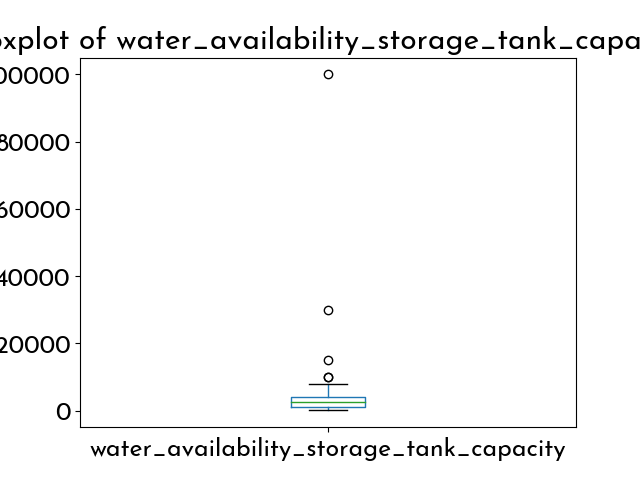
\includegraphics[scale=0.5]{/Users/chaix/Hedera/GIT/XLSform2PDF/output/svf/plots/graph_water_availability_storage_tank_capacity.png}
\end{figure}
\paragraph{How many times has the storage tank been filled in the last month? }
\  \\Variable name: \texttt{water\_availability\_storage\_tank\_filtered}\\
Type: integer\\
\\Total number of answers: 105 (42.9\%)
\\[0.2em] \begin{tabular}{p{4cm}|p{8cm}}
Minimum value &0.0 \\
\hline
\cellcolor{mygray} Maximum value & \cellcolor{mygray}2000.0 \\
\hline
Variance &37930.32271062271 \\
\hline
\cellcolor{mygray} Mean value & \cellcolor{mygray}24.419047619047618 \\
\hline
\end{tabular}
\begin{figure}[H]
\centering
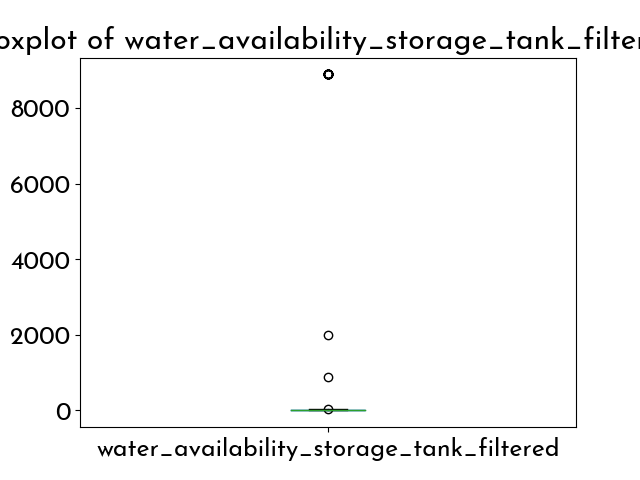
\includegraphics[scale=0.5]{/Users/chaix/Hedera/GIT/XLSform2PDF/output/svf/plots/graph_water_availability_storage_tank_filtered.png}
\end{figure}
\paragraph{Has there been any time in the last month when you have not been able to store sufficient water to meet your needs? }
\  \\Variable name: \texttt{water\_availability\_storage\_tank\_problems}\\
Type: single choice\\
\\Total number of answers: 154 (62.9\%)
\\[0.2em] \begin{tabular}{p{4cm}|p{8cm}|p{3cm}}
Choice code & Label & Answers \\
\hline
yes & Yes& \cellcolor{color3}94 (61.0\%)\\
\cellcolor{mygray} no & \cellcolor{mygray}No & \cellcolor{color1}59 (38.3\%)\\
99 & Don’t know& \cellcolor{color0}1 (0.6\%)\\
\end{tabular}
\paragraph{Can you show me the storage tank? Can I take a picture?}
\  \\Variable name: \texttt{water\_storage\_tank\_picture}\\
Type: image\\
\paragraph{Does your household store drinking water in small containers (capacity 50 liters or less)? }
\  \\Variable name: \texttt{water\_availability\_small\_tanks}\\
Type: single choice\\
\\Total number of answers: 243 (99.2\%)
\\[0.2em] \begin{tabular}{p{4cm}|p{8cm}|p{3cm}}
Choice code & Label & Answers \\
\hline
yes & Yes& \cellcolor{color4}211 (86.8\%)\\
\cellcolor{mygray} no & \cellcolor{mygray}No & \cellcolor{color0}32 (13.2\%)\\
\end{tabular}
\paragraph{Can you show me the storage tank? Can I take a picture?}
\  \\Variable name: \texttt{water\_small\_storage\_tank\_picture}\\
Type: image\\
\paragraph{Do you or another member of the household usually treat the water to make it safer to drink? }
\ \\ {\small For example: filtering, boiling, adding chemicals, disinfection (details can be given in the next question)}
\  \\Variable name: \texttt{water\_quality\_treated}\hfill\colorbox{red}{\small{\textcolor{white}{required}}}\\
 Type: single choice\\
\\Total number of answers: 245 (100.0\%)
\\[0.2em] \begin{tabular}{p{4cm}|p{8cm}|p{3cm}}
Choice code & Label & Answers \\
\hline
yes & Yes& \cellcolor{color3}162 (66.1\%)\\
\cellcolor{mygray} no & \cellcolor{mygray}No & \cellcolor{color1}83 (33.9\%)\\
\end{tabular}
\paragraph{What do you usually do to the water to make it safer to drink? }
\ \\ {\small Record all methods used. }
\  \\Variable name: \texttt{water\_quality\_treatments}\hfill\colorbox{red}{\small{\textcolor{white}{required}}}\\
 Type: multiple choice\\
\\Total number of answers: 162 (66.1\%)
\\[0.2em] \begin{tabular}{p{4cm}|p{8cm}|p{3cm}}
Choice code & Label & Answers \\
\hline
1 & Boil & \cellcolor{color3}128 (79.0\%)\\
\cellcolor{mygray} 2 & \cellcolor{mygray}Add bleach / chlorine  & \cellcolor{color0}5 (3.1\%)\\
3 & Strain it through a cloth & \cellcolor{color0}2 (1.2\%)\\
\cellcolor{mygray} 4 & \cellcolor{mygray}Use water filter (ceramic, sand, composite, reverse osmosis, etc.)  & \cellcolor{color0}23 (14.2\%)\\
5 & Solar disinfection & \cellcolor{color0}0 (0.0\%)\\
\cellcolor{mygray} 6 & \cellcolor{mygray}Let it stand and settle  & \cellcolor{color0}10 (6.2\%)\\
99 & Don’t know& \cellcolor{color0}0 (0.0\%)\\
\cellcolor{mygray} other & \cellcolor{mygray}Other & \cellcolor{color0}9 (5.6\%)\\
\end{tabular}
\paragraph{Please specify:}
\  \\Variable name: \texttt{water\_quality\_treatments\_other}\\
Type: text\\
\\Total number of answers: 162 (66.1\%)
\\[0.2em]\begin{table}[H]
 \begin{tabular}{p{4cm}|p{8cm}}
Word & Number of occurrences  \\
\hline
\cellcolor{mygray}drink&\cellcolor{mygray}7\\
\hline
without&4\\
\hline
\cellcolor{mygray}water&\cellcolor{mygray}2\\
\hline
directly&2\\
\hline
\cellcolor{mygray}step&\cellcolor{mygray}2\\
\hline
steps&2\\
\hline
\cellcolor{mygray}jibu&\cellcolor{mygray}1\\
\hline
drinking&1\\
\hline
\end{tabular}
\caption{\label{tab:table-name} Most used words for this answer}
\end{table}
\paragraph{What kind of toilet facility do members of your household usually use? }
\  \\Variable name: \texttt{sanitation\_toilet}\hfill\colorbox{red}{\small{\textcolor{white}{required}}}\\
 Type: single choice\\
\\Total number of answers: 245 (100.0\%)
\\[0.2em] \begin{tabular}{p{4cm}|p{8cm}|p{3cm}}
Choice code & Label & Answers \\
\hline
dry\_pit\_slab & Dry pit latrine with slab& \cellcolor{color0}24 (9.8\%)\\
\cellcolor{mygray} dry\_pit\_no\_slab & \cellcolor{mygray}Dry pit latrine without slab / Open pit & \cellcolor{color4}218 (89.0\%)\\
bucket & Bucket& \cellcolor{color0}0 (0.0\%)\\
\cellcolor{mygray} none & \cellcolor{mygray}No facility / Bush / Field  & \cellcolor{color0}0 (0.0\%)\\
flush\_piped & Flush - Flush to piped sewer system& \cellcolor{color0}0 (0.0\%)\\
\cellcolor{mygray} flush\_septic & \cellcolor{mygray}Flush - Flush to concrete/brick septic tank with 2 or more chambers & \cellcolor{color0}0 (0.0\%)\\
flush\_concrete & Flush - Flush to concrete/brick tank (one chamber)& \cellcolor{color0}0 (0.0\%)\\
\cellcolor{mygray} flush\_plastic & \cellcolor{mygray}Flush - Flush to plastic drum/tank & \cellcolor{color0}0 (0.0\%)\\
flush\_latrine & Flush - Flush to pit latrine& \cellcolor{color0}0 (0.0\%)\\
\cellcolor{mygray} flush\_open & \cellcolor{mygray}Flush - Flush to open drain & \cellcolor{color0}0 (0.0\%)\\
flush\_na & Flush - Flush to don’t know where& \cellcolor{color0}0 (0.0\%)\\
\cellcolor{mygray} flush\_elsewhere & \cellcolor{mygray}Flush - Flush to elsewhere  & \cellcolor{color0}0 (0.0\%)\\
twin\_pit\_slab & Composting toilet - Twin pit with slab& \cellcolor{color0}0 (0.0\%)\\
\cellcolor{mygray} twin\_pit\_no\_slap & \cellcolor{mygray}Composting toilet - Twin pit without slab & \cellcolor{color0}0 (0.0\%)\\
composting & Composting toilet - Other composting toilet& \cellcolor{color0}0 (0.0\%)\\
\cellcolor{mygray} container & \cellcolor{mygray}Container-based sanitation  & \cellcolor{color0}0 (0.0\%)\\
water\_body & Toilet connected to water body& \cellcolor{color0}0 (0.0\%)\\
\cellcolor{mygray} other & \cellcolor{mygray}Other  & \cellcolor{color0}3 (1.2\%)\\
\end{tabular}
\paragraph{Please, specify the toilet facility that the members of your household usually use}
\  \\Variable name: \texttt{sanitation\_toilet\_other}\\
Type: text\\
\\Total number of answers: 245 (100.0\%)
\\[0.2em]\begin{table}[H]
 \begin{tabular}{p{4cm}|p{8cm}}
Word & Number of occurrences  \\
\hline
\cellcolor{mygray}toilet&\cellcolor{mygray}5\\
\hline
already&2\\
\hline
\cellcolor{mygray}finish&\cellcolor{mygray}2\\
\hline
slab&2\\
\hline
\cellcolor{mygray}use&\cellcolor{mygray}1\\
\hline
home&1\\
\hline
\cellcolor{mygray}shop&\cellcolor{mygray}1\\
\hline
urgent&1\\
\hline
\end{tabular}
\caption{\label{tab:table-name} Most used words for this answer}
\end{table}
\paragraph{Where is the toilet facility located? }
\  \\Variable name: \texttt{sanitation\_accessibility\_location}\hfill\colorbox{red}{\small{\textcolor{white}{required}}}\\
 Type: single choice\\
\\Total number of answers: 245 (100.0\%)
\\[0.2em] \begin{tabular}{p{4cm}|p{8cm}|p{3cm}}
Choice code & Label & Answers \\
\hline
house & In own house& \cellcolor{color0}6 (2.4\%)\\
\cellcolor{mygray} yard & \cellcolor{mygray}In own yard/plot & \cellcolor{color4}236 (96.3\%)\\
lake & From a lake& \cellcolor{color0}0 (0.0\%)\\
\cellcolor{mygray} river & \cellcolor{mygray}From a river & \cellcolor{color0}0 (0.0\%)\\
other & Elsewhere& \cellcolor{color0}3 (1.2\%)\\
\end{tabular}
\paragraph{Please specify:}
\  \\Variable name: \texttt{sanitation\_accessibility\_location\_other}\\
Type: text\\
\\Total number of answers: 245 (100.0\%)
\\[0.2em]\begin{table}[H]
 \begin{tabular}{p{4cm}|p{8cm}}
Word & Number of occurrences  \\
\hline
\cellcolor{mygray}facility&\cellcolor{mygray}2\\
\hline
bit&1\\
\hline
\cellcolor{mygray}far&\cellcolor{mygray}1\\
\hline
house&1\\
\hline
\cellcolor{mygray}days&\cellcolor{mygray}1\\
\hline
digging&1\\
\hline
\cellcolor{mygray}new&\cellcolor{mygray}1\\
\hline
old&1\\
\hline
\end{tabular}
\caption{\label{tab:table-name} Most used words for this answer}
\end{table}
\paragraph{Is it possible for me to see the toilet facility? Can I take a photo?}
\  \\Variable name: \texttt{sanitation\_toilet\_image}\\
Type: image\\
\paragraph{Does your toilet ever overflow? }
\  \\Variable name: \texttt{sanitation\_containment\_leak}\\
Type: single choice\\
\\Total number of answers: 245 (100.0\%)
\\[0.2em] \begin{tabular}{p{4cm}|p{8cm}|p{3cm}}
Choice code & Label & Answers \\
\hline
1 & Never& \cellcolor{color4}209 (85.3\%)\\
\cellcolor{mygray} 2 & \cellcolor{mygray}Rarely & \cellcolor{color0}13 (5.3\%)\\
3 & Yes, sometimes& \cellcolor{color0}23 (9.4\%)\\
\cellcolor{mygray} 4 & \cellcolor{mygray}Yes, very frequently & \cellcolor{color0}0 (0.0\%)\\
5 & Yes, always& \cellcolor{color0}0 (0.0\%)\\
\end{tabular}
\paragraph{What is your septic tank connected to? Where does the liquid go?}
\  \\Variable name: \texttt{sanitation\_containment\_septic\_tank\_discharge}\\
Type: single choice\\
\paragraph{Please specify:}
\  \\Variable name: \texttt{sanitation\_containment\_septic\_tank\_discharge\_other}\\
Type: text\\
\\Total number of answers: 0 (0.0\%)
\\[0.2em]\paragraph{Do all household members usually use the toilet facility? Do the small children use it? Do the men use it?}
\  \\Variable name: \texttt{sanitation\_accessibility\_users}\hfill\colorbox{red}{\small{\textcolor{white}{required}}}\\
 Type: single choice\\
\\Total number of answers: 245 (100.0\%)
\\[0.2em] \begin{tabular}{p{4cm}|p{8cm}|p{3cm}}
Choice code & Label & Answers \\
\hline
yes & Yes& \cellcolor{color3}195 (79.6\%)\\
\cellcolor{mygray} no & \cellcolor{mygray}No & \cellcolor{color0}49 (20.0\%)\\
99 & Don’t know& \cellcolor{color0}1 (0.4\%)\\
\end{tabular}
\paragraph{Is everyone in the household able to access and use the toilet at all times of the day and night? }
\  \\Variable name: \texttt{sanitation\_accessibility\_toilet\_accessible}\\
Type: single choice\\
\\Total number of answers: 245 (100.0\%)
\\[0.2em] \begin{tabular}{p{4cm}|p{8cm}|p{3cm}}
Choice code & Label & Answers \\
\hline
yes & Yes& \cellcolor{color4}221 (90.2\%)\\
\cellcolor{mygray} no & \cellcolor{mygray}No & \cellcolor{color0}23 (9.4\%)\\
99 & Don’t know& \cellcolor{color0}1 (0.4\%)\\
\end{tabular}
\paragraph{What is the (main) reason that household members are unable to use the toilet at all times of the day or night? }
\  \\Variable name: \texttt{sanitation\_accessibility\_toilet\_accessible\_reason}\\
Type: single choice\\
\\Total number of answers: 23 (9.4\%)
\\[0.2em] \begin{tabular}{p{4cm}|p{8cm}|p{3cm}}
Choice code & Label & Answers \\
\hline
1 & Limited mobility prevents members from using the toilet.& \cellcolor{color0}1 (4.3\%)\\
\cellcolor{mygray} 2 & \cellcolor{mygray}Distance/barriers prevent members from reaching the toilet.  & \cellcolor{color0}2 (8.7\%)\\
3 & Toilet is not always available to all household members (e.g., men and women are not allowed to use the same toilet)& \cellcolor{color0}0 (0.0\%)\\
\cellcolor{mygray} 4 & \cellcolor{mygray}The toilet is not always safe for all members of the household. & \cellcolor{color4}19 (82.6\%)\\
other & Other& \cellcolor{color0}1 (4.3\%)\\
\end{tabular}
\paragraph{Please specify}
\  \\Variable name: \texttt{sanitation\_accessibility\_toilet\_accessible\_reason\_other}\\
Type: text\\
\\Total number of answers: 23 (9.4\%)
\\[0.2em]\begin{table}[H]
 \begin{tabular}{p{4cm}|p{8cm}}
Word & Number of occurrences  \\
\hline
\cellcolor{mygray}small&\cellcolor{mygray}1\\
\hline
child&1\\
\hline
\cellcolor{mygray}use&\cellcolor{mygray}1\\
\hline
\end{tabular}
\caption{\label{tab:table-name} Most used words for this answer}
\end{table}
\paragraph{Why do some household members not use the toilet facility, even though it is accessible?}
\  \\Variable name: \texttt{sanitaton\_accessibility\_non\_usage\_reason}\\
Type: text\\
\\Total number of answers: 23 (9.4\%)
\\[0.2em]\begin{table}[H]
 \begin{tabular}{p{4cm}|p{8cm}}
Word & Number of occurrences  \\
\hline
\cellcolor{mygray}child&\cellcolor{mygray}21\\
\hline
2&10\\
\hline
\cellcolor{mygray}year&\cellcolor{mygray}10\\
\hline
years&9\\
\hline
\cellcolor{mygray}1&\cellcolor{mygray}8\\
\hline
use&8\\
\hline
\cellcolor{mygray}old&\cellcolor{mygray}7\\
\hline
months&6\\
\hline
\end{tabular}
\caption{\label{tab:table-name} Most used words for this answer}
\end{table}
\paragraph{Has your toilet pit/septic tank/concrete tank ever been emptied? }
\  \\Variable name: \texttt{sanitation\_emptying\_is\_emptied}\hfill\colorbox{red}{\small{\textcolor{white}{required}}}\\
 Type: single choice\\
\\Total number of answers: 242 (98.8\%)
\\[0.2em] \begin{tabular}{p{4cm}|p{8cm}|p{3cm}}
Choice code & Label & Answers \\
\hline
yes & Yes, it has been emptied& \cellcolor{color1}53 (21.9\%)\\
\cellcolor{mygray} no & \cellcolor{mygray}No, never & \cellcolor{color3}189 (78.1\%)\\
99 & Don’t know& \cellcolor{color0}0 (0.0\%)\\
\end{tabular}
\paragraph{The last time it was emptied, who removed the content? }
\ \\ {\small This question is used to calculate proportion of households safely disposing of excreta in situ and the proportion removing excreta off-site for treatment.}
\  \\Variable name: \texttt{sanitation\_emptying\_who}\hfill\colorbox{red}{\small{\textcolor{white}{required}}}\\
 Type: single choice\\
\\Total number of answers: 53 (21.6\%)
\\[0.2em] \begin{tabular}{p{4cm}|p{8cm}|p{3cm}}
Choice code & Label & Answers \\
\hline
provider & Service provider& \cellcolor{color1}12 (22.6\%)\\
\cellcolor{mygray} household & \cellcolor{mygray}Household & \cellcolor{color0}5 (9.4\%)\\
na & Don’t know & \cellcolor{color0}0 (0.0\%)\\
\cellcolor{mygray} other & \cellcolor{mygray}Other  & \cellcolor{color3}36 (67.9\%)\\
\end{tabular}
\paragraph{The last time it was emptied, where was the waste disposed of? }
\  \\Variable name: \texttt{sanitation\_emptying\_where}\hfill\colorbox{red}{\small{\textcolor{white}{required}}}\\
 Type: single choice\\
\\Total number of answers: 53 (21.6\%)
\\[0.2em] \begin{tabular}{p{4cm}|p{8cm}|p{3cm}}
Choice code & Label & Answers \\
\hline
1 & Treatment plant& \cellcolor{color0}0 (0.0\%)\\
\cellcolor{mygray} 2 & \cellcolor{mygray}Buried in a covered pit & \cellcolor{color0}0 (0.0\%)\\
3 & Open drain, uncovered pit, open ground, water body, or elsewhere & \cellcolor{color0}0 (0.0\%)\\
\cellcolor{mygray} 4 & \cellcolor{mygray}Don’t know & \cellcolor{color0}0 (0.0\%)\\
\end{tabular}
\paragraph{The last time a child defecated, what was done to dispose of the feces? }
\ \\ {\small Note: to be answered only if there are children (<15 years old) in the household.}
\  \\Variable name: \texttt{sanitation\_waste\_disposal\_child\_stool}\\
Type: single choice\\
\\Total number of answers: 245 (100.0\%)
\\[0.2em] \begin{tabular}{p{4cm}|p{8cm}|p{3cm}}
Choice code & Label & Answers \\
\hline
1 & Child used toilet& \cellcolor{color2}147 (60.0\%)\\
\cellcolor{mygray} 2 & \cellcolor{mygray}Put/flushed into toilet or latrine  & \cellcolor{color1}67 (27.3\%)\\
3 & Put/flushed into drain or ditch & \cellcolor{color0}0 (0.0\%)\\
\cellcolor{mygray} 4 & \cellcolor{mygray}Mixed with other garbage (solid waste)  & \cellcolor{color0}0 (0.0\%)\\
5 & Buried & \cellcolor{color0}2 (0.8\%)\\
\cellcolor{mygray} 6 & \cellcolor{mygray}Left in the open  & \cellcolor{color0}0 (0.0\%)\\
7 & Used as manure & \cellcolor{color0}0 (0.0\%)\\
\cellcolor{mygray} na & \cellcolor{mygray}Don’t know  & \cellcolor{color0}0 (0.0\%)\\
other & Other & \cellcolor{color0}29 (11.8\%)\\
\end{tabular}
\paragraph{If you selected "Other", please specify:}
\  \\Variable name: \texttt{sanitation\_waste\_disposal\_child\_stool\_other}\\
Type: text\\
\\Total number of answers: 245 (100.0\%)
\\[0.2em]\begin{table}[H]
 \begin{tabular}{p{4cm}|p{8cm}}
Word & Number of occurrences  \\
\hline
\cellcolor{mygray}pit&\cellcolor{mygray}14\\
\hline
latrine&13\\
\hline
\cellcolor{mygray}disposed&\cellcolor{mygray}9\\
\hline
carried&8\\
\hline
\cellcolor{mygray}waste&\cellcolor{mygray}7\\
\hline
clothes&4\\
\hline
\cellcolor{mygray}lives&\cellcolor{mygray}4\\
\hline
dispose&4\\
\hline
\end{tabular}
\caption{\label{tab:table-name} Most used words for this answer}
\end{table}
\paragraph{How does your household usually dispose of solid waste (organic and non-organic)? }
\  \\Variable name: \texttt{sanitation\_waste\_disposal\_solid}\hfill\colorbox{red}{\small{\textcolor{white}{required}}}\\
 Type: multiple choice\\
\\Total number of answers: 245 (100.0\%)
\\[0.2em] \begin{tabular}{p{4cm}|p{8cm}|p{3cm}}
Choice code & Label & Answers \\
\hline
5 & Disposed of within household yard or plot & \cellcolor{color2}144 (58.8\%)\\
\cellcolor{mygray} 6 & \cellcolor{mygray}Buried or burned  & \cellcolor{color2}129 (52.7\%)\\
na & Don’t know & \cellcolor{color0}1 (0.4\%)\\
\cellcolor{mygray} other & \cellcolor{mygray}Disposed of elsewhere  & \cellcolor{color1}57 (23.3\%)\\
\end{tabular}
\paragraph{Please specify:}
\  \\Variable name: \texttt{sanitation\_waste\_disposal\_solid\_other}\\
Type: text\\
\\Total number of answers: 245 (100.0\%)
\\[0.2em]\begin{table}[H]
 \begin{tabular}{p{4cm}|p{8cm}}
Word & Number of occurrences  \\
\hline
\cellcolor{mygray}organic&\cellcolor{mygray}48\\
\hline
waste&29\\
\hline
\cellcolor{mygray}used&\cellcolor{mygray}28\\
\hline
farm&14\\
\hline
\cellcolor{mygray}fertiliser&\cellcolor{mygray}14\\
\hline
manure&13\\
\hline
\cellcolor{mygray}disposed&\cellcolor{mygray}10\\
\hline
trees&10\\
\hline
\end{tabular}
\caption{\label{tab:table-name} Most used words for this answer}
\end{table}
\paragraph{How do you dispose of household water used for cooking, laundry, and bathing? }
\  \\Variable name: \texttt{sanitation\_waste\_disposal\_liquid}\hfill\colorbox{red}{\small{\textcolor{white}{required}}}\\
 Type: multiple choice\\
\\Total number of answers: 245 (100.0\%)
\\[0.2em] \begin{tabular}{p{4cm}|p{8cm}|p{3cm}}
Choice code & Label & Answers \\
\hline
3 & Sink/drain connected to pit & \cellcolor{color0}1 (0.4\%)\\
\cellcolor{mygray} 4 & \cellcolor{mygray}Sink/drain connected to soak pit  & \cellcolor{color0}0 (0.0\%)\\
5 & Sink/drain connected to open drain or open ground & \cellcolor{color1}53 (21.6\%)\\
\cellcolor{mygray} 6 & \cellcolor{mygray}Disposed of directly in street/open ground/water body  & \cellcolor{color3}193 (78.8\%)\\
na & N/A (cooking, laundry, and bathing is done outside the household) & \cellcolor{color0}0 (0.0\%)\\
\cellcolor{mygray} 99 & \cellcolor{mygray}Don’t know  & \cellcolor{color0}1 (0.4\%)\\
\end{tabular}
\paragraph{Please specify:}
\  \\Variable name: \texttt{sanitation\_waste\_disposal\_liquid\_other}\\
Type: text\\
\\Total number of answers: 245 (100.0\%)
\\[0.2em]\paragraph{Do you share this facility only with members of other nearby households that you know, or is the facility open to the entire community/general public? }
\  \\Variable name: \texttt{sanitation\_acceptability\_shared\_toilet}\hfill\colorbox{red}{\small{\textcolor{white}{required}}}\\
 Type: single choice\\
\\Total number of answers: 245 (100.0\%)
\\[0.2em] \begin{tabular}{p{4cm}|p{8cm}|p{3cm}}
Choice code & Label & Answers \\
\hline
no & No, it is not shared& \cellcolor{color4}241 (98.4\%)\\
\cellcolor{mygray} household & \cellcolor{mygray}Shared with known households (not public)  & \cellcolor{color0}3 (1.2\%)\\
public & Shared with community/general public & \cellcolor{color0}1 (0.4\%)\\
\end{tabular}
\paragraph{How many households in total use this toilet facility, including your own household? }
\  \\Variable name: \texttt{sanitation\_acceptability\_shared\_toilet\_n\_hh}\\
Type: integer\\
\\Total number of answers: 3 (1.2\%)
\\[0.2em] \begin{tabular}{p{4cm}|p{8cm}}
Minimum value &2.0 \\
\hline
\cellcolor{mygray} Maximum value & \cellcolor{mygray}4.0 \\
\hline
Variance &1.3333333333333333 \\
\hline
\cellcolor{mygray} Mean value & \cellcolor{mygray}2.6666666666666665 \\
\hline
\end{tabular}
\begin{figure}[H]
\centering
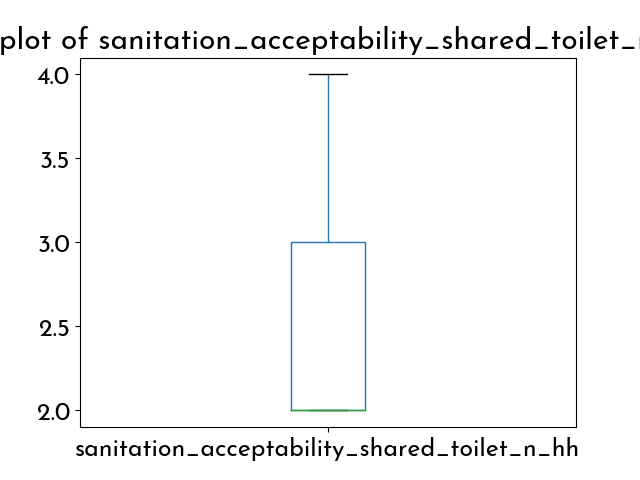
\includegraphics[scale=0.5]{/Users/chaix/Hedera/GIT/XLSform2PDF/output/svf/plots/graph_sanitation_acceptability_shared_toilet_n_hh.png}
\end{figure}
\paragraph{Does the design of your toilet prevent other people from seeing and hearing you when you use it? }
\  \\Variable name: \texttt{sanitation\_acceptability\_privacy}\\
Type: single choice\\
\\Total number of answers: 245 (100.0\%)
\\[0.2em] \begin{tabular}{p{4cm}|p{8cm}|p{3cm}}
Choice code & Label & Answers \\
\hline
yes & Yes& \cellcolor{color3}150 (61.2\%)\\
\cellcolor{mygray} no & \cellcolor{mygray}No & \cellcolor{color1}95 (38.8\%)\\
\end{tabular}
\paragraph{Do you or other household members face any risks when using the toilet? }
\ \\ {\small For instance, without light, far from home, insufficient hygiene.}
\  \\Variable name: \texttt{sanitation\_acceptability\_safety}\\
Type: single choice\\
\\Total number of answers: 244 (99.6\%)
\\[0.2em] \begin{tabular}{p{4cm}|p{8cm}|p{3cm}}
Choice code & Label & Answers \\
\hline
none & No risks faced & \cellcolor{color2}144 (59.0\%)\\
\cellcolor{mygray} health & \cellcolor{mygray}Yes, risk to health  & \cellcolor{color1}53 (21.7\%)\\
harassment & Yes, risk of harassment & \cellcolor{color0}0 (0.0\%)\\
\cellcolor{mygray} safety & \cellcolor{mygray}Yes, risk of safety & \cellcolor{color0}46 (18.9\%)\\
other & Yes, other & \cellcolor{color0}1 (0.4\%)\\
\end{tabular}
\paragraph{Please specify:}
\  \\Variable name: \texttt{sanitation\_acceptability\_safety\_other}\\
Type: text\\
\\Total number of answers: 244 (99.6\%)
\\[0.2em]\begin{table}[H]
 \begin{tabular}{p{4cm}|p{8cm}}
Word & Number of occurrences  \\
\hline
\cellcolor{mygray}shop&\cellcolor{mygray}1\\
\hline
\end{tabular}
\caption{\label{tab:table-name} Most used words for this answer}
\end{table}
\paragraph{Can you show me the place where household members most often wash their hands? }
\  \\Variable name: \texttt{hygiene\_handwashing\_shown}\hfill\colorbox{red}{\small{\textcolor{white}{required}}}\\
 Type: single choice\\
\\Total number of answers: 245 (100.0\%)
\\[0.2em] \begin{tabular}{p{4cm}|p{8cm}|p{3cm}}
Choice code & Label & Answers \\
\hline
yes & Yes& \cellcolor{color4}204 (83.3\%)\\
\cellcolor{mygray} no & \cellcolor{mygray}No & \cellcolor{color0}41 (16.7\%)\\
\end{tabular}
\paragraph{Can I take a photo of the handwashing place?}
\  \\Variable name: \texttt{hygiene\_handwashing\_image}\\
Type: image\\
\paragraph{Where do the members of your household most often wash their hands? }
\  \\Variable name: \texttt{hygiene\_handwashing}\hfill\colorbox{red}{\small{\textcolor{white}{required}}}\\
 Type: single choice\\
\\Total number of answers: 245 (100.0\%)
\\[0.2em] \begin{tabular}{p{4cm}|p{8cm}|p{3cm}}
Choice code & Label & Answers \\
\hline
mobile & Mobile device observed (bucket/jug/kettle)& \cellcolor{color4}222 (90.6\%)\\
\cellcolor{mygray} none & \cellcolor{mygray}No handwashing place in house/yard/plot  & \cellcolor{color0}13 (5.3\%)\\
fixed\_house & Fixed facility observed (sink/tap) - in house& \cellcolor{color0}3 (1.2\%)\\
\cellcolor{mygray} fixed\_yard & \cellcolor{mygray}Fixed facility observed (sink/tap) - in yard/plot & \cellcolor{color0}5 (2.0\%)\\
na & No permission to see& \cellcolor{color0}1 (0.4\%)\\
\cellcolor{mygray} other & \cellcolor{mygray}Other & \cellcolor{color0}1 (0.4\%)\\
\end{tabular}
\paragraph{Please specify}
\  \\Variable name: \texttt{hygiene\_handwashing\_other}\\
Type: text\\
\\Total number of answers: 245 (100.0\%)
\\[0.2em]\begin{table}[H]
 \begin{tabular}{p{4cm}|p{8cm}}
Word & Number of occurrences  \\
\hline
\cellcolor{mygray}use&\cellcolor{mygray}1\\
\hline
hand&1\\
\hline
\cellcolor{mygray}sanitizer&\cellcolor{mygray}1\\
\hline
\end{tabular}
\caption{\label{tab:table-name} Most used words for this answer}
\end{table}
\paragraph{When do you wash your hands?}
\ \\ {\small Select all that apply.}
\  \\Variable name: \texttt{hygiene\_handwashing\_activities}\\
Type: multiple choice\\
\\Total number of answers: 245 (100.0\%)
\\[0.2em] \begin{tabular}{p{4cm}|p{8cm}|p{3cm}}
Choice code & Label & Answers \\
\hline
1 & Before, during, \& after preparing food& \cellcolor{color3}184 (75.1\%)\\
\cellcolor{mygray} 2 & \cellcolor{mygray}Before eating food & \cellcolor{color4}243 (99.2\%)\\
3 & Before and after caring for someone at home who is sick& \cellcolor{color2}130 (53.1\%)\\
\cellcolor{mygray} 4 & \cellcolor{mygray}Before and after treating a cut or a wound & \cellcolor{color1}92 (37.6\%)\\
5 & After using the toilet& \cellcolor{color4}231 (94.3\%)\\
\cellcolor{mygray} other & \cellcolor{mygray}Other & \cellcolor{color0}5 (2.0\%)\\
\end{tabular}
\paragraph{Pease specify}
\  \\Variable name: \texttt{hygiene\_handwashing\_activities\_other}\\
Type: text\\
\\Total number of answers: 245 (100.0\%)
\\[0.2em]\begin{table}[H]
 \begin{tabular}{p{4cm}|p{8cm}}
Word & Number of occurrences  \\
\hline
\cellcolor{mygray}breast&\cellcolor{mygray}4\\
\hline
child&4\\
\hline
\cellcolor{mygray}giving&\cellcolor{mygray}3\\
\hline
going&1\\
\hline
\cellcolor{mygray}give&\cellcolor{mygray}1\\
\hline
befor&1\\
\hline
\cellcolor{mygray}client&\cellcolor{mygray}1\\
\hline
enter&1\\
\hline
\end{tabular}
\caption{\label{tab:table-name} Most used words for this answer}
\end{table}
\paragraph{Is there water available for handwashing when needed?}
\ \\ {\small If possible, verify by checking the tap/pump, or basin, bucket, water container, or similar objects for the presence of water. }
\  \\Variable name: \texttt{hygiene\_handwashing\_water\_available}\hfill\colorbox{red}{\small{\textcolor{white}{required}}}\\
 Type: single choice\\
\\Total number of answers: 245 (100.0\%)
\\[0.2em] \begin{tabular}{p{4cm}|p{8cm}|p{3cm}}
Choice code & Label & Answers \\
\hline
yes & Yes& \cellcolor{color4}224 (91.4\%)\\
\cellcolor{mygray} no & \cellcolor{mygray}No & \cellcolor{color0}21 (8.6\%)\\
\end{tabular}
\paragraph{Is there soap available?}
\  \\Variable name: \texttt{hygiene\_handwashing\_soap\_available}\hfill\colorbox{red}{\small{\textcolor{white}{required}}}\\
 Type: single choice\\
\\Total number of answers: 245 (100.0\%)
\\[0.2em] \begin{tabular}{p{4cm}|p{8cm}|p{3cm}}
Choice code & Label & Answers \\
\hline
yes & Yes& \cellcolor{color3}174 (71.0\%)\\
\cellcolor{mygray} no & \cellcolor{mygray}No & \cellcolor{color1}71 (29.0\%)\\
\end{tabular}
\paragraph{What kind of soap or material do you have in your household for handwashing? }
\ \\ {\small Direct observation of handwashing is challenging. The recommended proxy is to observe presence of handwashing facilities and availability of soap and water. If possible, observe the place of handwashing and record all that apply.}
\  \\Variable name: \texttt{hygiene\_handwashing\_soap}\\
Type: multiple choice\\
\\Total number of answers: 173 (70.6\%)
\\[0.2em] \begin{tabular}{p{4cm}|p{8cm}|p{3cm}}
Choice code & Label & Answers \\
\hline
1 & Bar or liquid soap& \cellcolor{color0}0 (0.0\%)\\
\cellcolor{mygray} 2 & \cellcolor{mygray}Detergent (powder, liquid, paste) & \cellcolor{color0}0 (0.0\%)\\
none & None / soap not shown& \cellcolor{color0}0 (0.0\%)\\
\cellcolor{mygray} other & \cellcolor{mygray}Other & \cellcolor{color0}0 (0.0\%)\\
\end{tabular}
\paragraph{Please specify the other soap material that you have in your household}
\  \\Variable name: \texttt{hygiene\_handwashing\_soap\_other}\\
Type: text\\
\\Total number of answers: 173 (70.6\%)
\\[0.2em]\newpage\section{Household Food Insecurity Experience Scale }
\paragraph{In the past 12 months, did you worry that your household would not have enough food?}
\  \\Variable name: \texttt{fies\_worried}\hfill\colorbox{red}{\small{\textcolor{white}{required}}}\\
 Type: single choice\\
\\Total number of answers: 245 (100.0\%)
\\[0.2em] \begin{tabular}{p{4cm}|p{8cm}|p{3cm}}
Choice code & Label & Answers \\
\hline
yes\_month & Yes, in the past month& \cellcolor{color1}87 (35.5\%)\\
\cellcolor{mygray} yes\_year & \cellcolor{mygray}Yes, in the past year but not in the last month & \cellcolor{color1}86 (35.1\%)\\
no & No& \cellcolor{color1}72 (29.4\%)\\
\end{tabular}
\paragraph{If yes, how often did this happen? }
\  \\Variable name: \texttt{fies\_worried\_frequency}\\
Type: single choice\\
\\Total number of answers: 173 (70.6\%)
\\[0.2em] \begin{tabular}{p{4cm}|p{8cm}|p{3cm}}
Choice code & Label & Answers \\
\hline
rarely & Rarely (once or twice in a typical month)& \cellcolor{color0}28 (16.2\%)\\
\cellcolor{mygray} sometimes & \cellcolor{mygray}Sometimes (three to ten times in a typical month) & \cellcolor{color2}75 (43.4\%)\\
often & Often (more than 10 times per month)& \cellcolor{color2}70 (40.5\%)\\
\end{tabular}
\paragraph{In the past 12 months, did it happen that you or any household member were not able to eat healthy and nutritious food? }
\ \\ {\small The definition of health and nutritious should be left up to the respondent according to his/her own perception.}
\  \\Variable name: \texttt{fies\_healthy}\hfill\colorbox{red}{\small{\textcolor{white}{required}}}\\
 Type: single choice\\
\\Total number of answers: 245 (100.0\%)
\\[0.2em] \begin{tabular}{p{4cm}|p{8cm}|p{3cm}}
Choice code & Label & Answers \\
\hline
yes\_month & Yes, in the past month& \cellcolor{color2}114 (46.5\%)\\
\cellcolor{mygray} yes\_year & \cellcolor{mygray}Yes, in the past year but not in the last month & \cellcolor{color1}85 (34.7\%)\\
no & No& \cellcolor{color0}46 (18.8\%)\\
\end{tabular}
\paragraph{If yes, how often did this happen? }
\  \\Variable name: \texttt{fies\_healthy\_frequency}\\
Type: single choice\\
\\Total number of answers: 198 (80.8\%)
\\[0.2em] \begin{tabular}{p{4cm}|p{8cm}|p{3cm}}
Choice code & Label & Answers \\
\hline
rarely & Rarely (once or twice in a typical month)& \cellcolor{color0}26 (13.1\%)\\
\cellcolor{mygray} sometimes & \cellcolor{mygray}Sometimes (three to ten times in a typical month) & \cellcolor{color1}61 (30.8\%)\\
often & Often (more than 10 times per month)& \cellcolor{color2}111 (56.1\%)\\
\end{tabular}
\paragraph{In the past 12 months, did it happen that you or any household member were not able to eat the kind of food you would have preferred to eat because of lack of resources?}
\  \\Variable name: \texttt{fies\_preferred}\hfill\colorbox{red}{\small{\textcolor{white}{required}}}\\
 Type: single choice\\
\\Total number of answers: 245 (100.0\%)
\\[0.2em] \begin{tabular}{p{4cm}|p{8cm}|p{3cm}}
Choice code & Label & Answers \\
\hline
yes\_month & Yes, in the past month& \cellcolor{color2}134 (54.7\%)\\
\cellcolor{mygray} yes\_year & \cellcolor{mygray}Yes, in the past year but not in the last month & \cellcolor{color1}94 (38.4\%)\\
no & No& \cellcolor{color0}17 (6.9\%)\\
\end{tabular}
\paragraph{If yes, how often did this happen? }
\  \\Variable name: \texttt{fies\_preferred\_frequency}\\
Type: single choice\\
\\Total number of answers: 228 (93.1\%)
\\[0.2em] \begin{tabular}{p{4cm}|p{8cm}|p{3cm}}
Choice code & Label & Answers \\
\hline
rarely & Rarely (once or twice in a typical month)& \cellcolor{color0}16 (7.0\%)\\
\cellcolor{mygray} sometimes & \cellcolor{mygray}Sometimes (three to ten times in a typical month) & \cellcolor{color1}72 (31.6\%)\\
often & Often (more than 10 times per month)& \cellcolor{color3}140 (61.4\%)\\
\end{tabular}
\paragraph{In the past 12 months, did it happen that you or any household member had to eat a limited variety of foods because of lack of resources? }
\  \\Variable name: \texttt{fies\_fewfood}\hfill\colorbox{red}{\small{\textcolor{white}{required}}}\\
 Type: single choice\\
\\Total number of answers: 245 (100.0\%)
\\[0.2em] \begin{tabular}{p{4cm}|p{8cm}|p{3cm}}
Choice code & Label & Answers \\
\hline
yes\_month & Yes, in the past month& \cellcolor{color2}125 (51.0\%)\\
\cellcolor{mygray} yes\_year & \cellcolor{mygray}Yes, in the past year but not in the last month & \cellcolor{color1}95 (38.8\%)\\
no & No& \cellcolor{color0}25 (10.2\%)\\
\end{tabular}
\paragraph{If yes, how often did this happen? }
\  \\Variable name: \texttt{fies\_fewfood\_frequency}\\
Type: single choice\\
\\Total number of answers: 220 (89.8\%)
\\[0.2em] \begin{tabular}{p{4cm}|p{8cm}|p{3cm}}
Choice code & Label & Answers \\
\hline
rarely & Rarely (once or twice in a typical month)& \cellcolor{color0}17 (7.7\%)\\
\cellcolor{mygray} sometimes & \cellcolor{mygray}Sometimes (three to ten times in a typical month) & \cellcolor{color1}78 (35.5\%)\\
often & Often (more than 10 times per month)& \cellcolor{color2}125 (56.8\%)\\
\end{tabular}
\paragraph{In the past 12 months, did it happen that you or any household member had to eat some foods that you really did not want to eat because of lack of resources? }
\  \\Variable name: \texttt{fies\_unwanted}\hfill\colorbox{red}{\small{\textcolor{white}{required}}}\\
 Type: single choice\\
\\Total number of answers: 245 (100.0\%)
\\[0.2em] \begin{tabular}{p{4cm}|p{8cm}|p{3cm}}
Choice code & Label & Answers \\
\hline
yes\_month & Yes, in the past month& \cellcolor{color2}129 (52.7\%)\\
\cellcolor{mygray} yes\_year & \cellcolor{mygray}Yes, in the past year but not in the last month & \cellcolor{color1}89 (36.3\%)\\
no & No& \cellcolor{color0}27 (11.0\%)\\
\end{tabular}
\paragraph{If yes, how often did this happen? }
\  \\Variable name: \texttt{fies\_unwanted\_frequency}\\
Type: single choice\\
\\Total number of answers: 216 (88.2\%)
\\[0.2em] \begin{tabular}{p{4cm}|p{8cm}|p{3cm}}
Choice code & Label & Answers \\
\hline
rarely & Rarely (once or twice in a typical month)& \cellcolor{color0}18 (8.3\%)\\
\cellcolor{mygray} sometimes & \cellcolor{mygray}Sometimes (three to ten times in a typical month) & \cellcolor{color1}79 (36.6\%)\\
often & Often (more than 10 times per month)& \cellcolor{color2}119 (55.1\%)\\
\end{tabular}
\paragraph{In the past 12 months, did it happen that you or any household member had to skip a meal because there was not enough food? }
\  \\Variable name: \texttt{fies\_skipped}\hfill\colorbox{red}{\small{\textcolor{white}{required}}}\\
 Type: single choice\\
\\Total number of answers: 245 (100.0\%)
\\[0.2em] \begin{tabular}{p{4cm}|p{8cm}|p{3cm}}
Choice code & Label & Answers \\
\hline
yes\_month & Yes, in the past month& \cellcolor{color1}70 (28.6\%)\\
\cellcolor{mygray} yes\_year & \cellcolor{mygray}Yes, in the past year but not in the last month & \cellcolor{color1}62 (25.3\%)\\
no & No& \cellcolor{color2}113 (46.1\%)\\
\end{tabular}
\paragraph{If yes, how often did this happen? }
\  \\Variable name: \texttt{fies\_skipped\_frequency}\\
Type: single choice\\
\\Total number of answers: 132 (53.9\%)
\\[0.2em] \begin{tabular}{p{4cm}|p{8cm}|p{3cm}}
Choice code & Label & Answers \\
\hline
rarely & Rarely (once or twice in a typical month)& \cellcolor{color0}21 (15.9\%)\\
\cellcolor{mygray} sometimes & \cellcolor{mygray}Sometimes (three to ten times in a typical month) & \cellcolor{color2}64 (48.5\%)\\
often & Often (more than 10 times per month)& \cellcolor{color1}47 (35.6\%)\\
\end{tabular}
\paragraph{In the past 12 months, did it happen that you or any household member had to eat a smaller meal than you felt you needed because there was not enough food? }
\  \\Variable name: \texttt{fies\_ateless}\hfill\colorbox{red}{\small{\textcolor{white}{required}}}\\
 Type: single choice\\
\\Total number of answers: 245 (100.0\%)
\\[0.2em] \begin{tabular}{p{4cm}|p{8cm}|p{3cm}}
Choice code & Label & Answers \\
\hline
yes\_month & Yes, in the past month& \cellcolor{color2}110 (44.9\%)\\
\cellcolor{mygray} yes\_year & \cellcolor{mygray}Yes, in the past year but not in the last month & \cellcolor{color1}74 (30.2\%)\\
no & No& \cellcolor{color1}61 (24.9\%)\\
\end{tabular}
\paragraph{If yes, how often did this happen? }
\  \\Variable name: \texttt{fies\_ateless\_frequency}\\
Type: single choice\\
\\Total number of answers: 184 (75.1\%)
\\[0.2em] \begin{tabular}{p{4cm}|p{8cm}|p{3cm}}
Choice code & Label & Answers \\
\hline
rarely & Rarely (once or twice in a typical month)& \cellcolor{color0}15 (8.2\%)\\
\cellcolor{mygray} sometimes & \cellcolor{mygray}Sometimes (three to ten times in a typical month) & \cellcolor{color2}81 (44.0\%)\\
often & Often (more than 10 times per month)& \cellcolor{color2}88 (47.8\%)\\
\end{tabular}
\paragraph{In the past 12 months, did it happen that there was no food to eat of any kind in your house, because of lack of resources to get food? }
\  \\Variable name: \texttt{fies\_runout}\hfill\colorbox{red}{\small{\textcolor{white}{required}}}\\
 Type: single choice\\
\\Total number of answers: 245 (100.0\%)
\\[0.2em] \begin{tabular}{p{4cm}|p{8cm}|p{3cm}}
Choice code & Label & Answers \\
\hline
yes\_month & Yes, in the past month& \cellcolor{color1}67 (27.3\%)\\
\cellcolor{mygray} yes\_year & \cellcolor{mygray}Yes, in the past year but not in the last month & \cellcolor{color1}71 (29.0\%)\\
no & No& \cellcolor{color2}107 (43.7\%)\\
\end{tabular}
\paragraph{If yes, how often did this happen? }
\  \\Variable name: \texttt{fies\_runout\_frequency}\\
Type: single choice\\
\\Total number of answers: 137 (55.9\%)
\\[0.2em] \begin{tabular}{p{4cm}|p{8cm}|p{3cm}}
Choice code & Label & Answers \\
\hline
rarely & Rarely (once or twice in a typical month)& \cellcolor{color0}17 (12.4\%)\\
\cellcolor{mygray} sometimes & \cellcolor{mygray}Sometimes (three to ten times in a typical month) & \cellcolor{color2}59 (43.1\%)\\
often & Often (more than 10 times per month)& \cellcolor{color2}61 (44.5\%)\\
\end{tabular}
\paragraph{Please describe what did you do in this situation.}
\ \\ {\small (Maximum 1200 characters)}
\  \\Variable name: \texttt{fies\_runout\_explain}\\
Type: text\\
\\Total number of answers: 137 (55.9\%)
\\[0.2em]\begin{table}[H]
 \begin{tabular}{p{4cm}|p{8cm}}
Word & Number of occurrences  \\
\hline
\cellcolor{mygray}went&\cellcolor{mygray}15\\
\hline
food&14\\
\hline
\cellcolor{mygray}search&\cellcolor{mygray}14\\
\hline
job&9\\
\hline
\cellcolor{mygray}get&\cellcolor{mygray}7\\
\hline
eat&7\\
\hline
\cellcolor{mygray}cook&\cellcolor{mygray}6\\
\hline
work&6\\
\hline
\end{tabular}
\caption{\label{tab:table-name} Most used words for this answer}
\end{table}
\paragraph{In the past 12 months, did it happen that you or any household were hungry but could not eat because there was not enough food? }
\  \\Variable name: \texttt{fies\_hungry}\hfill\colorbox{red}{\small{\textcolor{white}{required}}}\\
 Type: single choice\\
\\Total number of answers: 245 (100.0\%)
\\[0.2em] \begin{tabular}{p{4cm}|p{8cm}|p{3cm}}
Choice code & Label & Answers \\
\hline
yes\_month & Yes, in the past month& \cellcolor{color1}90 (36.7\%)\\
\cellcolor{mygray} yes\_year & \cellcolor{mygray}Yes, in the past year but not in the last month & \cellcolor{color1}62 (25.3\%)\\
no & No& \cellcolor{color1}93 (38.0\%)\\
\end{tabular}
\paragraph{If yes, how often did this happen? }
\  \\Variable name: \texttt{fies\_hungry\_yes}\\
Type: single choice\\
\\Total number of answers: 150 (61.2\%)
\\[0.2em] \begin{tabular}{p{4cm}|p{8cm}|p{3cm}}
Choice code & Label & Answers \\
\hline
rarely & Rarely (once or twice in a typical month)& \cellcolor{color0}26 (17.3\%)\\
\cellcolor{mygray} sometimes & \cellcolor{mygray}Sometimes (three to ten times in a typical month) & \cellcolor{color1}58 (38.7\%)\\
often & Often (more than 10 times per month)& \cellcolor{color2}66 (44.0\%)\\
\end{tabular}
\paragraph{Please describe what did you do in this situation.}
\ \\ {\small (Maximum 1200 characters)}
\  \\Variable name: \texttt{fies\_hungry\_explain}\\
Type: text\\
\\Total number of answers: 150 (61.2\%)
\\[0.2em]\begin{table}[H]
 \begin{tabular}{p{4cm}|p{8cm}}
Word & Number of occurrences  \\
\hline
\cellcolor{mygray}food&\cellcolor{mygray}21\\
\hline
wait&18\\
\hline
\cellcolor{mygray}patient&\cellcolor{mygray}14\\
\hline
went&13\\
\hline
\cellcolor{mygray}search&\cellcolor{mygray}13\\
\hline
cook&9\\
\hline
\cellcolor{mygray}job&\cellcolor{mygray}9\\
\hline
ready&9\\
\hline
\end{tabular}
\caption{\label{tab:table-name} Most used words for this answer}
\end{table}
\paragraph{In the past 12 months, did it happen that you or any household member went a whole day and night without eating anything at all because there was not enough food?}
\  \\Variable name: \texttt{fies\_wholeday}\hfill\colorbox{red}{\small{\textcolor{white}{required}}}\\
 Type: single choice\\
\\Total number of answers: 245 (100.0\%)
\\[0.2em] \begin{tabular}{p{4cm}|p{8cm}|p{3cm}}
Choice code & Label & Answers \\
\hline
yes\_month & Yes, in the past month& \cellcolor{color0}19 (7.8\%)\\
\cellcolor{mygray} yes\_year & \cellcolor{mygray}Yes, in the past year but not in the last month & \cellcolor{color0}17 (6.9\%)\\
no & No& \cellcolor{color4}209 (85.3\%)\\
\end{tabular}
\paragraph{If yes, how often did this happen? }
\  \\Variable name: \texttt{fies\_wholeday\_frequency}\\
Type: single choice\\
\\Total number of answers: 36 (14.7\%)
\\[0.2em] \begin{tabular}{p{4cm}|p{8cm}|p{3cm}}
Choice code & Label & Answers \\
\hline
rarely & Rarely (once or twice in a typical month)& \cellcolor{color1}14 (38.9\%)\\
\cellcolor{mygray} sometimes & \cellcolor{mygray}Sometimes (three to ten times in a typical month) & \cellcolor{color1}14 (38.9\%)\\
often & Often (more than 10 times per month)& \cellcolor{color1}8 (22.2\%)\\
\end{tabular}
\paragraph{Please describe what did you do in this situation.}
\ \\ {\small (Maximum 1200 caractères)}
\  \\Variable name: \texttt{fies\_wholeday\_explain}\\
Type: text\\
\\Total number of answers: 36 (14.7\%)
\\[0.2em]\begin{table}[H]
 \begin{tabular}{p{4cm}|p{8cm}}
Word & Number of occurrences  \\
\hline
\cellcolor{mygray}went&\cellcolor{mygray}5\\
\hline
work&4\\
\hline
\cellcolor{mygray}get&\cellcolor{mygray}4\\
\hline
food&3\\
\hline
\cellcolor{mygray}neighbors&\cellcolor{mygray}3\\
\hline
ask&3\\
\hline
\cellcolor{mygray}search&\cellcolor{mygray}3\\
\hline
something&2\\
\hline
\end{tabular}
\caption{\label{tab:table-name} Most used words for this answer}
\end{table}
\newpage\section{Household Dietary Diversity Score}
\paragraph{Did you or anyone in the household drink or eat cereals?E.g., rice, wheat, maize, sorghum, millet or any other grains or foods made from these, such as kawunga, bread, noodles, porridge, or other grain products.}
\  \\Variable name: \texttt{dietary\_cereals\_short}\\
Type: single choice\\
\\Total number of answers: 245 (100.0\%)
\\[0.2em] \begin{tabular}{p{4cm}|p{8cm}|p{3cm}}
Choice code & Label & Answers \\
\hline
yes & Yes& \cellcolor{color3}164 (66.9\%)\\
\cellcolor{mygray} no & \cellcolor{mygray}No & \cellcolor{color1}81 (33.1\%)\\
\end{tabular}
\paragraph{Did you or anyone in the household drink or eat yellow or orange coloured vegetables?E.g., pumpkin, carrot, squash, or sweet potato that are yellow or orange inside, or other locally available vitamin A rich vegetables (e.g. pumpkin flower).}
\  \\Variable name: \texttt{dietary\_vitamins\_a\_vegetables\_short}\\
Type: single choice\\
\\Total number of answers: 241 (98.4\%)
\\[0.2em] \begin{tabular}{p{4cm}|p{8cm}|p{3cm}}
Choice code & Label & Answers \\
\hline
yes & Yes& \cellcolor{color2}122 (50.6\%)\\
\cellcolor{mygray} no & \cellcolor{mygray}No & \cellcolor{color2}119 (49.4\%)\\
\end{tabular}
\paragraph{Did you or anyone in the household drink or eat white tubers? E.g., irish potatoes, sweet potatoes - white inside-, yams, cassava or food made from roots such as ubugali, kawunga, etc.}
\  \\Variable name: \texttt{dietary\_white\_tubers\_short}\\
Type: single choice\\
\\Total number of answers: 244 (99.6\%)
\\[0.2em] \begin{tabular}{p{4cm}|p{8cm}|p{3cm}}
Choice code & Label & Answers \\
\hline
yes & Yes& \cellcolor{color4}207 (84.8\%)\\
\cellcolor{mygray} no & \cellcolor{mygray}No & \cellcolor{color0}37 (15.2\%)\\
\end{tabular}
\paragraph{Did you or anyone in the household drink or eat dark green leafy vegetables?E.g., dodo, isombe, epinard/spinach, umushogoro, ibisusa, kale or others.}
\  \\Variable name: \texttt{dietary\_leafy\_veggie\_short}\\
Type: single choice\\
\\Total number of answers: 244 (99.6\%)
\\[0.2em] \begin{tabular}{p{4cm}|p{8cm}|p{3cm}}
Choice code & Label & Answers \\
\hline
yes & Yes& \cellcolor{color4}214 (87.7\%)\\
\cellcolor{mygray} no & \cellcolor{mygray}No & \cellcolor{color0}30 (12.3\%)\\
\end{tabular}
\paragraph{Did you or anyone in the household drink or eat other vegetables like those mentioned before? E.g., tomatoes, onions, eggplants.}
\  \\Variable name: \texttt{dietary\_other\_vegg\_short}\\
Type: single choice\\
\\Total number of answers: 244 (99.6\%)
\\[0.2em] \begin{tabular}{p{4cm}|p{8cm}|p{3cm}}
Choice code & Label & Answers \\
\hline
yes & Yes& \cellcolor{color3}173 (70.9\%)\\
\cellcolor{mygray} no & \cellcolor{mygray}No & \cellcolor{color1}71 (29.1\%)\\
\end{tabular}
\paragraph{Did you or anyone in the household drink or eat yellow or orange coloured fruits?E.g., ripe mangoes, papayas, passion fruits, tree tomatoes etc.}
\  \\Variable name: \texttt{dietary\_vitamins\_fruits\_short}\\
Type: single choice\\
\\Total number of answers: 244 (99.6\%)
\\[0.2em] \begin{tabular}{p{4cm}|p{8cm}|p{3cm}}
Choice code & Label & Answers \\
\hline
yes & Yes& \cellcolor{color1}50 (20.5\%)\\
\cellcolor{mygray} no & \cellcolor{mygray}No & \cellcolor{color3}194 (79.5\%)\\
\end{tabular}
\paragraph{Did you or anyone in the household drink or eat other fruits than those mentioned before (not yellowish/orange)?}
\  \\Variable name: \texttt{dietary\_other\_fruits\_short}\\
Type: single choice\\
\\Total number of answers: 245 (100.0\%)
\\[0.2em] \begin{tabular}{p{4cm}|p{8cm}|p{3cm}}
Choice code & Label & Answers \\
\hline
yes & Yes& \cellcolor{color1}52 (21.2\%)\\
\cellcolor{mygray} no & \cellcolor{mygray}No & \cellcolor{color3}193 (78.8\%)\\
\end{tabular}
\paragraph{Did you or anyone in the household drink or eat flesh meat? E.g., beef, pork, lamb, goat, rabbit, chicken, duck or other birds, etc.}
\  \\Variable name: \texttt{dietary\_meat\_short}\\
Type: single choice\\
\\Total number of answers: 245 (100.0\%)
\\[0.2em] \begin{tabular}{p{4cm}|p{8cm}|p{3cm}}
Choice code & Label & Answers \\
\hline
yes & Yes& \cellcolor{color0}33 (13.5\%)\\
\cellcolor{mygray} no & \cellcolor{mygray}No & \cellcolor{color4}212 (86.5\%)\\
\end{tabular}
\paragraph{Did you or anyone in the household eat organ meat? E.g., liver, kidney, heart or other organ meats or blood based food.}
\  \\Variable name: \texttt{dietary\_organ\_meat\_short}\\
Type: single choice\\
\\Total number of answers: 245 (100.0\%)
\\[0.2em] \begin{tabular}{p{4cm}|p{8cm}|p{3cm}}
Choice code & Label & Answers \\
\hline
yes & Yes& \cellcolor{color0}24 (9.8\%)\\
\cellcolor{mygray} no & \cellcolor{mygray}No & \cellcolor{color4}221 (90.2\%)\\
\end{tabular}
\paragraph{Did you or anyone in the household drink or eat fishE.g., fresh fish, dried fish, sambaza, crab, shrimps or shellfish, etc.}
\  \\Variable name: \texttt{dietary\_fish\_short}\\
Type: single choice\\
\\Total number of answers: 245 (100.0\%)
\\[0.2em] \begin{tabular}{p{4cm}|p{8cm}|p{3cm}}
Choice code & Label & Answers \\
\hline
yes & Yes& \cellcolor{color1}72 (29.4\%)\\
\cellcolor{mygray} no & \cellcolor{mygray}No & \cellcolor{color3}173 (70.6\%)\\
\end{tabular}
\paragraph{Did you or anyone in the household drink or eat legumes, nuts or seeds? E.g., beans, peas, soy, lentils, peanuts, nuts, seeds or food made of seeds such as peanut butter, etc.}
\  \\Variable name: \texttt{dietary\_nuts\_short}\\
Type: single choice\\
\\Total number of answers: 245 (100.0\%)
\\[0.2em] \begin{tabular}{p{4cm}|p{8cm}|p{3cm}}
Choice code & Label & Answers \\
\hline
yes & Yes& \cellcolor{color4}221 (90.2\%)\\
\cellcolor{mygray} no & \cellcolor{mygray}No & \cellcolor{color0}24 (9.8\%)\\
\end{tabular}
\paragraph{Did you or anyone in the household drink or eat milk or milk productsE.g., milk (inshushu), cheese, yoghurt, fermented milk (ikivuguto) or others}
\  \\Variable name: \texttt{dietary\_milky\_short}\\
Type: single choice\\
\\Total number of answers: 244 (99.6\%)
\\[0.2em] \begin{tabular}{p{4cm}|p{8cm}|p{3cm}}
Choice code & Label & Answers \\
\hline
yes & Yes& \cellcolor{color0}46 (18.9\%)\\
\cellcolor{mygray} no & \cellcolor{mygray}No & \cellcolor{color4}198 (81.1\%)\\
\end{tabular}
\paragraph{Did you or anyone in the household drink or eat oil and fats?E.g., oil, fats or butter added to food or used for cooking.}
\  \\Variable name: \texttt{dietary\_oils\_short}\\
Type: single choice\\
\\Total number of answers: 245 (100.0\%)
\\[0.2em] \begin{tabular}{p{4cm}|p{8cm}|p{3cm}}
Choice code & Label & Answers \\
\hline
yes & Yes& \cellcolor{color3}192 (78.4\%)\\
\cellcolor{mygray} no & \cellcolor{mygray}No & \cellcolor{color1}53 (21.6\%)\\
\end{tabular}
\paragraph{Did you or anyone in the household drink or eat sweets?E.g., sugar, honey, sweetened soda or sweetened juice drinks, sugary foods such as chocolates, candies, cookies and cakes.}
\  \\Variable name: \texttt{dietary\_sweets\_short}\\
Type: single choice\\
\\Total number of answers: 244 (99.6\%)
\\[0.2em] \begin{tabular}{p{4cm}|p{8cm}|p{3cm}}
Choice code & Label & Answers \\
\hline
yes & Yes& \cellcolor{color2}109 (44.7\%)\\
\cellcolor{mygray} no & \cellcolor{mygray}No & \cellcolor{color2}135 (55.3\%)\\
\end{tabular}
\paragraph{Did you or anyone in the household drink or eat spices, condiments, coffee, tea, or alcoholic beverages?}
\  \\Variable name: \texttt{dietary\_spices\_short}\\
Type: single choice\\
\\Total number of answers: 245 (100.0\%)
\\[0.2em] \begin{tabular}{p{4cm}|p{8cm}|p{3cm}}
Choice code & Label & Answers \\
\hline
yes & Yes& \cellcolor{color2}108 (44.1\%)\\
\cellcolor{mygray} no & \cellcolor{mygray}No & \cellcolor{color2}137 (55.9\%)\\
\end{tabular}
\newpage\section{Household Socio-Demographic Questionnaire}
\paragraph{Gender of respondent}
\  \\Variable name: \texttt{household\_gender}\hfill\colorbox{red}{\small{\textcolor{white}{required}}}\\
 Type: single choice\\
\\Total number of answers: 245 (100.0\%)
\\[0.2em] \begin{tabular}{p{4cm}|p{8cm}|p{3cm}}
Choice code & Label & Answers \\
\hline
W & Female& \cellcolor{color3}148 (60.4\%)\\
\cellcolor{mygray} M & \cellcolor{mygray}Male & \cellcolor{color1}97 (39.6\%)\\
O & Other (non-binary, gender-fluid, agender)& \cellcolor{color0}0 (0.0\%)\\
\cellcolor{mygray} P & \cellcolor{mygray}Prefer not to say & \cellcolor{color0}0 (0.0\%)\\
\end{tabular}
\paragraph{Marital Status}
\  \\Variable name: \texttt{household\_maritalstatus}\\
Type: single choice\\
\\Total number of answers: 245 (100.0\%)
\\[0.2em] \begin{tabular}{p{4cm}|p{8cm}|p{3cm}}
Choice code & Label & Answers \\
\hline
single & Single& \cellcolor{color0}13 (5.3\%)\\
\cellcolor{mygray} married & \cellcolor{mygray}Married  & \cellcolor{color3}164 (66.9\%)\\
divorced & Divorced& \cellcolor{color0}17 (6.9\%)\\
\cellcolor{mygray} partnered & \cellcolor{mygray}Partnered & \cellcolor{color0}14 (5.7\%)\\
widow & Widow& \cellcolor{color0}37 (15.1\%)\\
\end{tabular}
\paragraph{Age }
\  \\Variable name: \texttt{household\_age}\hfill\colorbox{red}{\small{\textcolor{white}{required}}}\\
 Type: single choice\\
\\Total number of answers: 245 (100.0\%)
\\[0.2em] \begin{tabular}{p{4cm}|p{8cm}|p{3cm}}
Choice code & Label & Answers \\
\hline
1 & 18-29& \cellcolor{color0}47 (19.2\%)\\
\cellcolor{mygray} 2 & \cellcolor{mygray}30-39 & \cellcolor{color1}64 (26.1\%)\\
3 & 40-49& \cellcolor{color0}43 (17.6\%)\\
\cellcolor{mygray} 4 & \cellcolor{mygray}50-64 & \cellcolor{color1}51 (20.8\%)\\
5 & 65-74& \cellcolor{color0}21 (8.6\%)\\
\cellcolor{mygray} 6 & \cellcolor{mygray}75+ & \cellcolor{color0}19 (7.8\%)\\
\end{tabular}
\paragraph{Would you like to provide your telephone number for a future assessment?}
\  \\Variable name: \texttt{household\_phone}\\
Type: text\\
\\Total number of answers: 245 (100.0\%)
\\[0.2em]\begin{table}[H]
 \begin{tabular}{p{4cm}|p{8cm}}
Word & Number of occurrences  \\
\hline
\cellcolor{mygray}0787717665&\cellcolor{mygray}2\\
\hline
0787408824&1\\
\hline
\cellcolor{mygray}0782064704&\cellcolor{mygray}1\\
\hline
0787834771&1\\
\hline
\cellcolor{mygray}0783490491&\cellcolor{mygray}1\\
\hline
0789613885&1\\
\hline
\cellcolor{mygray}0783984221&\cellcolor{mygray}1\\
\hline
0784099599&1\\
\hline
\end{tabular}
\caption{\label{tab:table-name} Most used words for this answer}
\end{table}
\paragraph{What is the hightest level of education somebody in the household completed?}
\  \\Variable name: \texttt{household\_education\_level}\\
Type: single choice\\
\\Total number of answers: 245 (100.0\%)
\\[0.2em] \begin{tabular}{p{4cm}|p{8cm}|p{3cm}}
Choice code & Label & Answers \\
\hline
primary & Primary& \cellcolor{color3}168 (68.6\%)\\
\cellcolor{mygray} high\_school & \cellcolor{mygray}Junior High School & \cellcolor{color0}15 (6.1\%)\\
senior\_high\_school & Senior High School (Plus Two - 12th)& \cellcolor{color0}12 (4.9\%)\\
\cellcolor{mygray} undergraduate & \cellcolor{mygray}Undergraduate & \cellcolor{color0}3 (1.2\%)\\
bachelor & Bachelor& \cellcolor{color0}0 (0.0\%)\\
\cellcolor{mygray} master & \cellcolor{mygray}Master & \cellcolor{color0}0 (0.0\%)\\
technical & Technical or professional degree& \cellcolor{color0}0 (0.0\%)\\
\cellcolor{mygray} phd & \cellcolor{mygray}PhD & \cellcolor{color0}0 (0.0\%)\\
none & None& \cellcolor{color0}45 (18.4\%)\\
\cellcolor{mygray} other & \cellcolor{mygray}Other & \cellcolor{color0}2 (0.8\%)\\
\end{tabular}
\paragraph{Please specify:}
\  \\Variable name: \texttt{household\_education\_level\_other}\\
Type: text\\
\\Total number of answers: 245 (100.0\%)
\\[0.2em]\begin{table}[H]
 \begin{tabular}{p{4cm}|p{8cm}}
Word & Number of occurrences  \\
\hline
\cellcolor{mygray}years&\cellcolor{mygray}4\\
\hline
6&2\\
\hline
\cellcolor{mygray}primary&\cellcolor{mygray}2\\
\hline
2&2\\
\hline
\cellcolor{mygray}school&\cellcolor{mygray}2\\
\hline
driver&1\\
\hline
\cellcolor{mygray}mechanic&\cellcolor{mygray}1\\
\hline
tailoring&1\\
\hline
\end{tabular}
\caption{\label{tab:table-name} Most used words for this answer}
\end{table}
\paragraph{Did you leave school before completing your education?}
\  \\Variable name: \texttt{household\_left\_school}\\
Type: single choice\\
\\Total number of answers: 220 (89.8\%)
\\[0.2em] \begin{tabular}{p{4cm}|p{8cm}|p{3cm}}
Choice code & Label & Answers \\
\hline
yes & Yes& \cellcolor{color3}163 (74.1\%)\\
\cellcolor{mygray} no & \cellcolor{mygray}No & \cellcolor{color1}57 (25.9\%)\\
\end{tabular}
\paragraph{How many years of school (in total) did you attend?}
\  \\Variable name: \texttt{household\_school\_years}\\
Type: integer\\
\\Total number of answers: 163 (66.5\%)
\\[0.2em] \begin{tabular}{p{4cm}|p{8cm}}
Minimum value &0.0 \\
\hline
\cellcolor{mygray} Maximum value & \cellcolor{mygray}12.0 \\
\hline
Variance &4.656820419601605 \\
\hline
\cellcolor{mygray} Mean value & \cellcolor{mygray}4.54601226993865 \\
\hline
\end{tabular}
\begin{figure}[H]
\centering
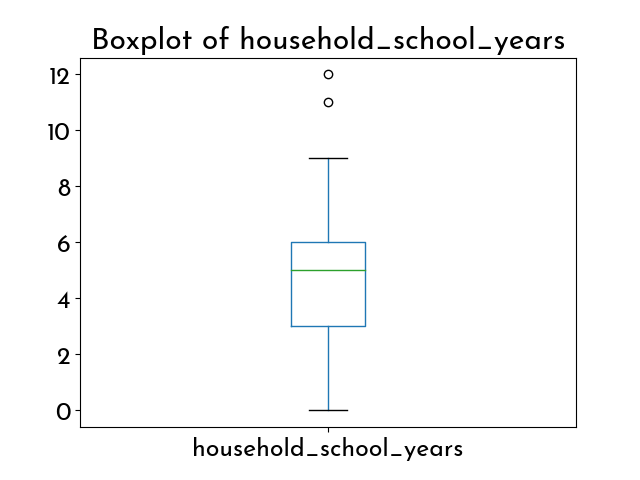
\includegraphics[scale=0.5]{/Users/chaix/Hedera/GIT/XLSform2PDF/output/svf/plots/graph_household_school_years.png}
\end{figure}
\paragraph{Why did you leave the school?}
\  \\Variable name: \texttt{household\_left\_school\_why}\\
Type: text\\
\\Total number of answers: 220 (89.8\%)
\\[0.2em]\begin{table}[H]
 \begin{tabular}{p{4cm}|p{8cm}}
Word & Number of occurrences  \\
\hline
\cellcolor{mygray}school&\cellcolor{mygray}62\\
\hline
lack&49\\
\hline
\cellcolor{mygray}fees&\cellcolor{mygray}38\\
\hline
parents&23\\
\hline
\cellcolor{mygray}family&\cellcolor{mygray}16\\
\hline
poverty&15\\
\hline
\cellcolor{mygray}activities&\cellcolor{mygray}15\\
\hline
poor&12\\
\hline
\end{tabular}
\caption{\label{tab:table-name} Most used words for this answer}
\end{table}
\paragraph{Are you or would  someone in your household be interested in a 2-weeks training to become either a sales person or a technician for solar systems?}
\  \\Variable name: \texttt{household\_training}\hfill\colorbox{red}{\small{\textcolor{white}{required}}}\\
 Type: single choice\\
\\Total number of answers: 245 (100.0\%)
\\[0.2em] \begin{tabular}{p{4cm}|p{8cm}|p{3cm}}
Choice code & Label & Answers \\
\hline
yes & Yes& \cellcolor{color2}119 (48.6\%)\\
\cellcolor{mygray} no & \cellcolor{mygray}No & \cellcolor{color2}126 (51.4\%)\\
\end{tabular}
\paragraph{Can the respondent read and write?}
\  \\Variable name: \texttt{household\_literacy}\\
Type: single choice\\
\\Total number of answers: 227 (92.7\%)
\\[0.2em] \begin{tabular}{p{4cm}|p{8cm}|p{3cm}}
Choice code & Label & Answers \\
\hline
yes & Yes& \cellcolor{color3}155 (68.3\%)\\
\cellcolor{mygray} no & \cellcolor{mygray}No & \cellcolor{color1}72 (31.7\%)\\
\end{tabular}
\paragraph{To which religion is the household affiliated ?}
\  \\Variable name: \texttt{household\_religion}\\
Type: single choice\\
\\Total number of answers: 245 (100.0\%)
\\[0.2em] \begin{tabular}{p{4cm}|p{8cm}|p{3cm}}
Choice code & Label & Answers \\
\hline
catholic & Catholic& \cellcolor{color2}133 (54.3\%)\\
\cellcolor{mygray} protestant & \cellcolor{mygray}Protestants & \cellcolor{color1}58 (23.7\%)\\
catholic\_other & Other Christian Beliefs& \cellcolor{color0}40 (16.3\%)\\
\cellcolor{mygray} muslim & \cellcolor{mygray}Muslim & \cellcolor{color0}1 (0.4\%)\\
indigeneous & Indigenous & \cellcolor{color0}0 (0.0\%)\\
\cellcolor{mygray} none & \cellcolor{mygray}None & \cellcolor{color0}3 (1.2\%)\\
na & Do not answer& \cellcolor{color0}0 (0.0\%)\\
\cellcolor{mygray} other & \cellcolor{mygray}Other & \cellcolor{color0}10 (4.1\%)\\
\end{tabular}
\paragraph{Please specify:}
\  \\Variable name: \texttt{household\_religion\_other}\\
Type: text\\
\\Total number of answers: 245 (100.0\%)
\\[0.2em]\begin{table}[H]
 \begin{tabular}{p{4cm}|p{8cm}}
Word & Number of occurrences  \\
\hline
\cellcolor{mygray}adventist&\cellcolor{mygray}5\\
\hline
advantist&3\\
\hline
\cellcolor{mygray}anglican&\cellcolor{mygray}2\\
\hline
\end{tabular}
\caption{\label{tab:table-name} Most used words for this answer}
\end{table}
\paragraph{Number of people living in the household}
\  \\Variable name: \texttt{household\_size}\hfill\colorbox{red}{\small{\textcolor{white}{required}}}\\
 Type: integer\\
\\Total number of answers: 199 (81.2\%)
\\[0.2em] \begin{tabular}{p{4cm}|p{8cm}}
Minimum value &1.0 \\
\hline
\cellcolor{mygray} Maximum value & \cellcolor{mygray}12.0 \\
\hline
Variance &4.3518603116593075 \\
\hline
\cellcolor{mygray} Mean value & \cellcolor{mygray}4.64321608040201 \\
\hline
\end{tabular}
\begin{figure}[H]
\centering
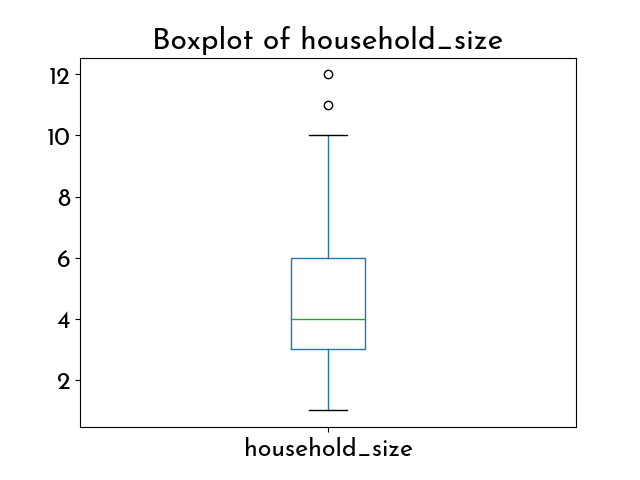
\includegraphics[scale=0.5]{/Users/chaix/Hedera/GIT/XLSform2PDF/output/svf/plots/graph_household_size.png}
\end{figure}
\paragraph{Men (16 years old or older) }
\  \\Variable name: \texttt{household\_men}\\
Type: integer\\
\\Total number of answers: 197 (80.4\%)
\\[0.2em] \begin{tabular}{p{4cm}|p{8cm}}
Minimum value &0.0 \\
\hline
\cellcolor{mygray} Maximum value & \cellcolor{mygray}10.0 \\
\hline
Variance &3.1711903035325806 \\
\hline
\cellcolor{mygray} Mean value & \cellcolor{mygray}1.6700507614213198 \\
\hline
\end{tabular}
\begin{figure}[H]
\centering
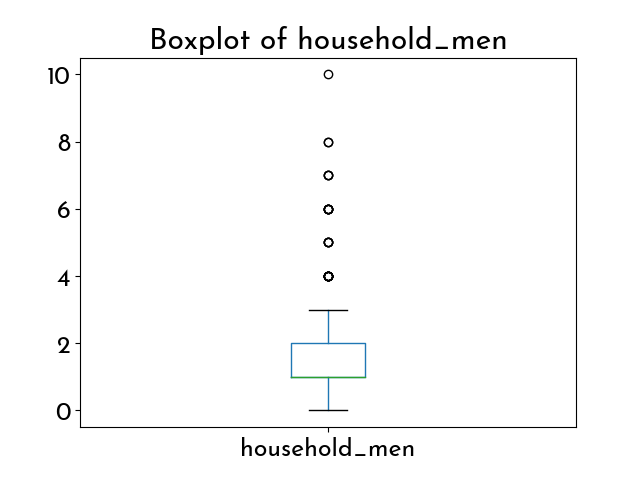
\includegraphics[scale=0.5]{/Users/chaix/Hedera/GIT/XLSform2PDF/output/svf/plots/graph_household_men.png}
\end{figure}
\paragraph{Women (16 years old or older) }
\  \\Variable name: \texttt{household\_women}\\
Type: integer\\
\\Total number of answers: 192 (78.4\%)
\\[0.2em] \begin{tabular}{p{4cm}|p{8cm}}
Minimum value &0.0 \\
\hline
\cellcolor{mygray} Maximum value & \cellcolor{mygray}4.0 \\
\hline
Variance &0.33963241710296677 \\
\hline
\cellcolor{mygray} Mean value & \cellcolor{mygray}1.3072916666666667 \\
\hline
\end{tabular}
\begin{figure}[H]
\centering
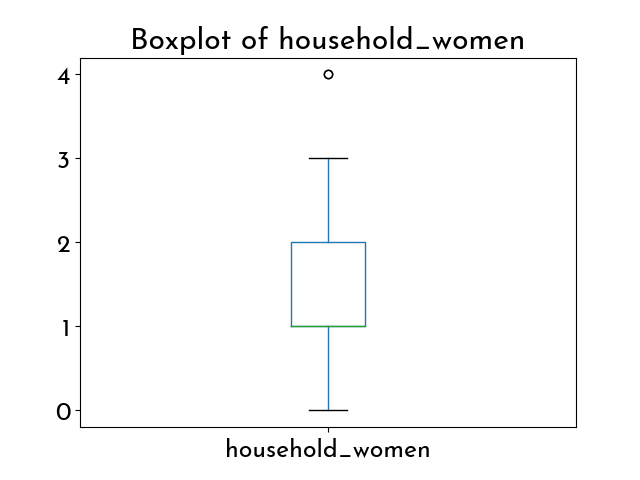
\includegraphics[scale=0.5]{/Users/chaix/Hedera/GIT/XLSform2PDF/output/svf/plots/graph_household_women.png}
\end{figure}
\paragraph{People 12 to 15 years old }
\  \\Variable name: \texttt{household\_adolescent}\\
Type: integer\\
\\Total number of answers: 113 (46.1\%)
\\[0.2em] \begin{tabular}{p{4cm}|p{8cm}}
Minimum value &0.0 \\
\hline
\cellcolor{mygray} Maximum value & \cellcolor{mygray}5.0 \\
\hline
Variance &1.038558786346397 \\
\hline
\cellcolor{mygray} Mean value & \cellcolor{mygray}1.2035398230088497 \\
\hline
\end{tabular}
\begin{figure}[H]
\centering
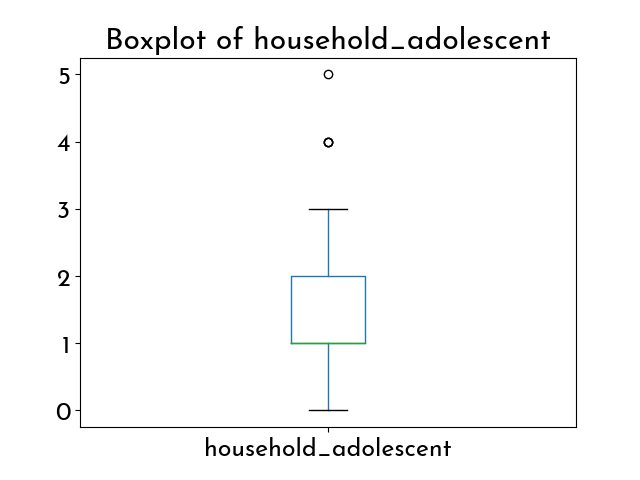
\includegraphics[scale=0.5]{/Users/chaix/Hedera/GIT/XLSform2PDF/output/svf/plots/graph_household_adolescent.png}
\end{figure}
\paragraph{Children between 5 and 11 years old}
\  \\Variable name: \texttt{household\_children}\\
Type: integer\\
\\Total number of answers: 133 (54.3\%)
\\[0.2em] \begin{tabular}{p{4cm}|p{8cm}}
Minimum value &0.0 \\
\hline
\cellcolor{mygray} Maximum value & \cellcolor{mygray}4.0 \\
\hline
Variance &0.7674868990658464 \\
\hline
\cellcolor{mygray} Mean value & \cellcolor{mygray}1.255639097744361 \\
\hline
\end{tabular}
\begin{figure}[H]
\centering
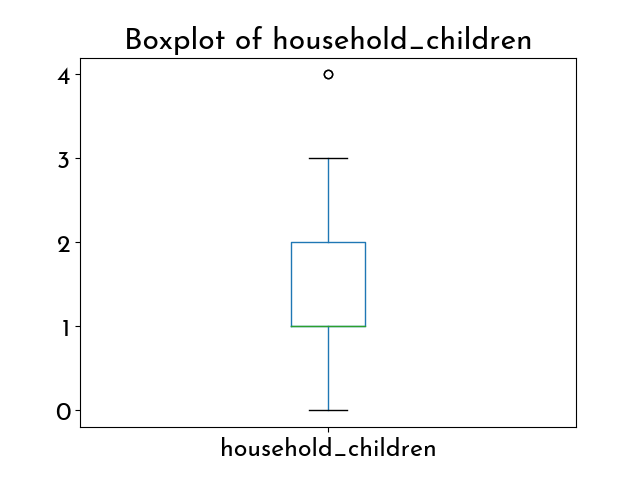
\includegraphics[scale=0.5]{/Users/chaix/Hedera/GIT/XLSform2PDF/output/svf/plots/graph_household_children.png}
\end{figure}
\paragraph{Children younger than 5}
\  \\Variable name: \texttt{household\_small\_children}\\
Type: integer\\
\\Total number of answers: 128 (52.2\%)
\\[0.2em] \begin{tabular}{p{4cm}|p{8cm}}
Minimum value &0.0 \\
\hline
\cellcolor{mygray} Maximum value & \cellcolor{mygray}3.0 \\
\hline
Variance &0.484251968503937 \\
\hline
\cellcolor{mygray} Mean value & \cellcolor{mygray}0.9375 \\
\hline
\end{tabular}
\begin{figure}[H]
\centering
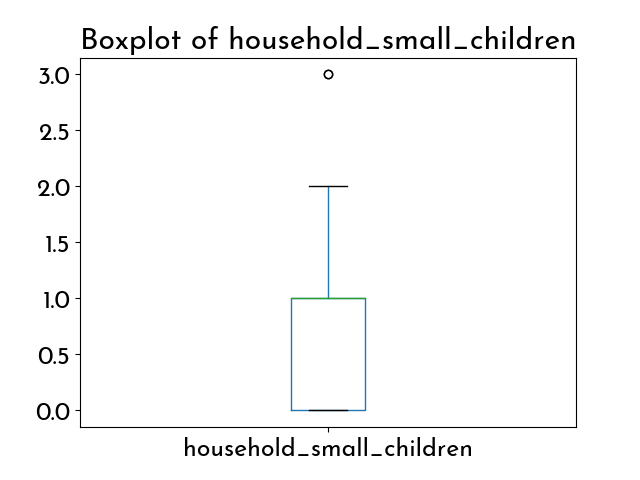
\includegraphics[scale=0.5]{/Users/chaix/Hedera/GIT/XLSform2PDF/output/svf/plots/graph_household_small_children.png}
\end{figure}
\paragraph{Is the house rented or owned?}
\  \\Variable name: \texttt{household\_ownership}\hfill\colorbox{red}{\small{\textcolor{white}{required}}}\\
 Type: single choice\\
\\Total number of answers: 202 (82.4\%)
\\[0.2em] \begin{tabular}{p{4cm}|p{8cm}|p{3cm}}
Choice code & Label & Answers \\
\hline
rented & Rented& \cellcolor{color0}25 (12.4\%)\\
\cellcolor{mygray} owned & \cellcolor{mygray}Owned & \cellcolor{color4}177 (87.6\%)\\
na & Do not answer& \cellcolor{color0}0 (0.0\%)\\
\end{tabular}
\paragraph{Number of rooms}
\  \\Variable name: \texttt{household\_rooms}\\
Type: integer\\
\\Total number of answers: 245 (100.0\%)
\\[0.2em] \begin{tabular}{p{4cm}|p{8cm}}
Minimum value &1 \\
\hline
\cellcolor{mygray} Maximum value & \cellcolor{mygray}11 \\
\hline
Variance &4.293074606891937 \\
\hline
\cellcolor{mygray} Mean value & \cellcolor{mygray}3.6530612244897958 \\
\hline
\end{tabular}
\begin{figure}[H]
\centering
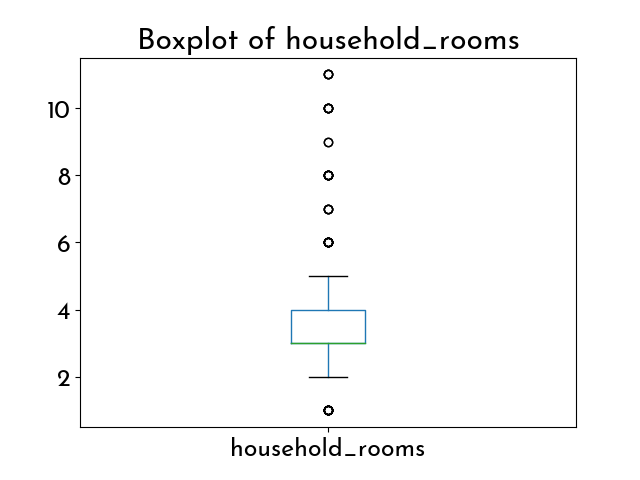
\includegraphics[scale=0.5]{/Users/chaix/Hedera/GIT/XLSform2PDF/output/svf/plots/graph_household_rooms.png}
\end{figure}
\paragraph{What is the main occupation of the household?}
\  \\Variable name: \texttt{household\_main\_occupation}\\
Type: single choice\\
\\Total number of answers: 245 (100.0\%)
\\[0.2em] \begin{tabular}{p{4cm}|p{8cm}|p{3cm}}
Choice code & Label & Answers \\
\hline
farming & Agriculture (Crop, Vegetables, Livestock, Forestry, Fishing)& \cellcolor{color4}218 (89.0\%)\\
\cellcolor{mygray} services & \cellcolor{mygray}Service business & \cellcolor{color0}2 (0.8\%)\\
commerce & Trading business& \cellcolor{color0}3 (1.2\%)\\
\cellcolor{mygray} mining & \cellcolor{mygray}Mining & \cellcolor{color0}0 (0.0\%)\\
constuction & Construction& \cellcolor{color0}1 (0.4\%)\\
\cellcolor{mygray} engineer & \cellcolor{mygray}Professional, engineering, scientific or technical activities & \cellcolor{color0}0 (0.0\%)\\
health & Health/Doctor or social work& \cellcolor{color0}0 (0.0\%)\\
\cellcolor{mygray} education & \cellcolor{mygray}Education/Teacher & \cellcolor{color0}4 (1.6\%)\\
public & Government/Administrative& \cellcolor{color0}0 (0.0\%)\\
\cellcolor{mygray} military & \cellcolor{mygray}Military / Security & \cellcolor{color0}0 (0.0\%)\\
employee & Private sector employee& \cellcolor{color0}0 (0.0\%)\\
\cellcolor{mygray} unskilled & \cellcolor{mygray}Unskilled worker & \cellcolor{color0}0 (0.0\%)\\
housewife & Unpaid domestic work& \cellcolor{color0}0 (0.0\%)\\
\cellcolor{mygray} retired & \cellcolor{mygray}Retired & \cellcolor{color0}3 (1.2\%)\\
unemployed & Unemployed& \cellcolor{color0}0 (0.0\%)\\
\cellcolor{mygray} other & \cellcolor{mygray}Other & \cellcolor{color0}14 (5.7\%)\\
\end{tabular}
\paragraph{Please specify}
\  \\Variable name: \texttt{household\_main\_occupation\_other}\\
Type: text\\
\\Total number of answers: 245 (100.0\%)
\\[0.2em]\begin{table}[H]
 \begin{tabular}{p{4cm}|p{8cm}}
Word & Number of occurrences  \\
\hline
\cellcolor{mygray}jobs&\cellcolor{mygray}9\\
\hline
small&7\\
\hline
\cellcolor{mygray}daily&\cellcolor{mygray}7\\
\hline
day&7\\
\hline
\cellcolor{mygray}searching&\cellcolor{mygray}3\\
\hline
looks&2\\
\hline
\cellcolor{mygray}food&\cellcolor{mygray}2\\
\hline
get&2\\
\hline
\end{tabular}
\caption{\label{tab:table-name} Most used words for this answer}
\end{table}
\paragraph{What is the income category of the household?}
\  \\Variable name: \texttt{household\_income\_category}\hfill\colorbox{red}{\small{\textcolor{white}{required}}}\\
 Type: single choice\\
\\Total number of answers: 245 (100.0\%)
\\[0.2em] \begin{tabular}{p{4cm}|p{8cm}|p{3cm}}
Choice code & Label & Answers \\
\hline
1 & Ubudehe category 1& \cellcolor{color0}35 (14.3\%)\\
\cellcolor{mygray} 2 & \cellcolor{mygray}Ubudehe category 2 & \cellcolor{color1}76 (31.0\%)\\
3 & Ubudehe category 3& \cellcolor{color2}126 (51.4\%)\\
\cellcolor{mygray} 4 & \cellcolor{mygray}Ubudehe category 4 & \cellcolor{color0}0 (0.0\%)\\
other & Other& \cellcolor{color0}8 (3.3\%)\\
\end{tabular}
\paragraph{Please specify:}
\  \\Variable name: \texttt{household\_income\_category\_other}\\
Type: text\\
\\Total number of answers: 245 (100.0\%)
\\[0.2em]\begin{table}[H]
 \begin{tabular}{p{4cm}|p{8cm}}
Word & Number of occurrences  \\
\hline
\cellcolor{mygray}category&\cellcolor{mygray}5\\
\hline
yet&4\\
\hline
\cellcolor{mygray}doesnt&\cellcolor{mygray}2\\
\hline
newlyweds&2\\
\hline
\cellcolor{mygray}registered&\cellcolor{mygray}2\\
\hline
waiting&1\\
\hline
\cellcolor{mygray}get&\cellcolor{mygray}1\\
\hline
new&1\\
\hline
\end{tabular}
\caption{\label{tab:table-name} Most used words for this answer}
\end{table}
\paragraph{Number of working women in the household}
\  \\Variable name: \texttt{household\_working\_female}\\
Type: integer\\
\\Total number of answers: 244 (99.6\%)
\\[0.2em] \begin{tabular}{p{4cm}|p{8cm}}
Minimum value &0.0 \\
\hline
\cellcolor{mygray} Maximum value & \cellcolor{mygray}4.0 \\
\hline
Variance &0.3975409836065573 \\
\hline
\cellcolor{mygray} Mean value & \cellcolor{mygray}0.7745901639344263 \\
\hline
\end{tabular}
\begin{figure}[H]
\centering
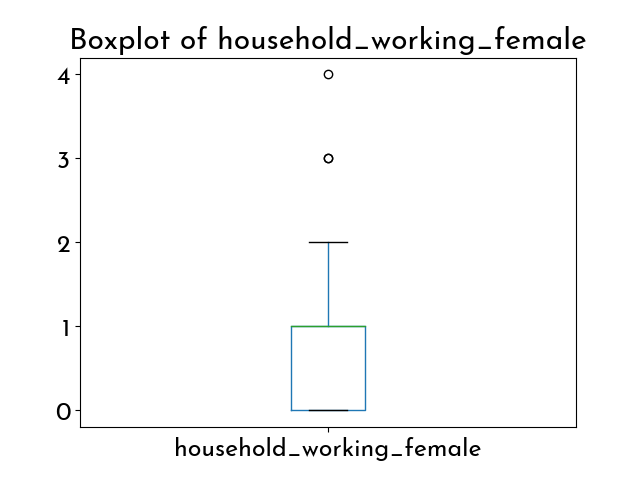
\includegraphics[scale=0.5]{/Users/chaix/Hedera/GIT/XLSform2PDF/output/svf/plots/graph_household_working_female.png}
\end{figure}
\paragraph{Number of working men in the household}
\  \\Variable name: \texttt{household\_working\_male}\\
Type: integer\\
\\Total number of answers: 242 (98.8\%)
\\[0.2em] \begin{tabular}{p{4cm}|p{8cm}}
Minimum value &0.0 \\
\hline
\cellcolor{mygray} Maximum value & \cellcolor{mygray}3.0 \\
\hline
Variance &0.4462809917355371 \\
\hline
\cellcolor{mygray} Mean value & \cellcolor{mygray}0.6694214876033058 \\
\hline
\end{tabular}
\begin{figure}[H]
\centering
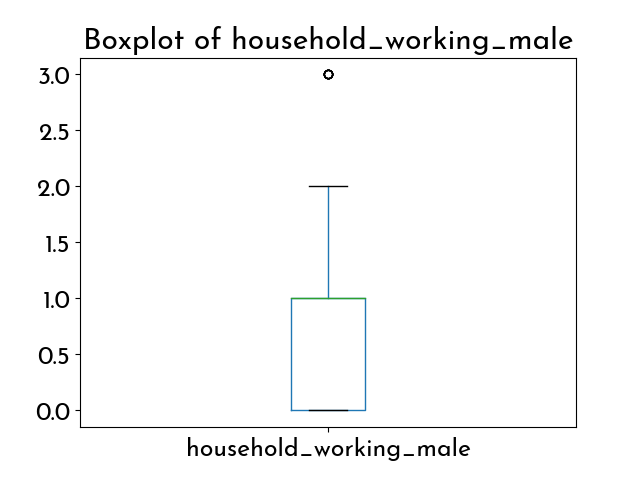
\includegraphics[scale=0.5]{/Users/chaix/Hedera/GIT/XLSform2PDF/output/svf/plots/graph_household_working_male.png}
\end{figure}
\paragraph{Total average monthly expenses of the household }
\ \\ {\small [in LOCAL currency]}
\  \\Variable name: \texttt{household\_monthly\_expenses}\hfill\colorbox{red}{\small{\textcolor{white}{required}}}\\
 Type: single choice\\
\\Total number of answers: 245 (100.0\%)
\\[0.2em] \begin{tabular}{p{4cm}|p{8cm}|p{3cm}}
Choice code & Label & Answers \\
\hline
1 & 45 000 RWF and below& \cellcolor{color3}162 (66.1\%)\\
\cellcolor{mygray} 2 & \cellcolor{mygray}45 001 RWF - 100 000 RWF & \cellcolor{color1}69 (28.2\%)\\
3 & 100 001 RWF - 300 000 RWF& \cellcolor{color0}14 (5.7\%)\\
\cellcolor{mygray} 4 & \cellcolor{mygray}300 001 RWF - 600 000 RWF & \cellcolor{color0}0 (0.0\%)\\
5 & Above 600 000 RWF& \cellcolor{color0}0 (0.0\%)\\
\end{tabular}
\paragraph{Are you member of one of the following organisations or groups?}
\  \\Variable name: \texttt{household\_member\_of}\hfill\colorbox{red}{\small{\textcolor{white}{required}}}\\
 Type: multiple choice\\
\\Total number of answers: 245 (100.0\%)
\\[0.2em] \begin{tabular}{p{4cm}|p{8cm}|p{3cm}}
Choice code & Label & Answers \\
\hline
sacco & Yes, SACCO& \cellcolor{color1}70 (28.6\%)\\
\cellcolor{mygray} cooperative & \cellcolor{mygray}Cooperatives & \cellcolor{color0}25 (10.2\%)\\
saving & Saving group& \cellcolor{color1}59 (24.1\%)\\
\cellcolor{mygray} selfhelp & \cellcolor{mygray}Other self-help group & \cellcolor{color1}82 (33.5\%)\\
none & None& \cellcolor{color1}62 (25.3\%)\\
\end{tabular}
\paragraph{Please specify:}
\  \\Variable name: \texttt{other\_member\_of}\\
Type: text\\
\\Total number of answers: 245 (100.0\%)
\\[0.2em]\begin{table}[H]
 \begin{tabular}{p{4cm}|p{8cm}}
Word & Number of occurrences  \\
\hline
\cellcolor{mygray}amatsinda&\cellcolor{mygray}28\\
\hline
group&19\\
\hline
\cellcolor{mygray}community&\cellcolor{mygray}14\\
\hline
help&13\\
\hline
\cellcolor{mygray}self&\cellcolor{mygray}10\\
\hline
saving&10\\
\hline
\cellcolor{mygray}association&\cellcolor{mygray}10\\
\hline
belong&8\\
\hline
\end{tabular}
\caption{\label{tab:table-name} Most used words for this answer}
\end{table}
\paragraph{How many saving groups are you member of?}
\  \\Variable name: \texttt{household\_n\_saving\_groups}\hfill\colorbox{red}{\small{\textcolor{white}{required}}}\\
 Type: single choice\\
\\Total number of answers: 59 (24.1\%)
\\[0.2em] \begin{tabular}{p{4cm}|p{8cm}|p{3cm}}
Choice code & Label & Answers \\
\hline
1 & 1& \cellcolor{color2}33 (55.9\%)\\
\cellcolor{mygray} 2 & \cellcolor{mygray}2 & \cellcolor{color1}22 (37.3\%)\\
3 & 3& \cellcolor{color0}3 (5.1\%)\\
\cellcolor{mygray} 4 & \cellcolor{mygray}4 & \cellcolor{color0}0 (0.0\%)\\
5 & 5& \cellcolor{color0}0 (0.0\%)\\
\cellcolor{mygray} 5+ & \cellcolor{mygray}More than 5 & \cellcolor{color0}1 (1.7\%)\\
\end{tabular}
\paragraph{What is the number of members of the biggest savings group you are part of?}
\  \\Variable name: \texttt{household\_saving\_group\_size}\hfill\colorbox{red}{\small{\textcolor{white}{required}}}\\
 Type: single choice\\
\\Total number of answers: 59 (24.1\%)
\\[0.2em] \begin{tabular}{p{4cm}|p{8cm}|p{3cm}}
Choice code & Label & Answers \\
\hline
10\_below & Less than 10& \cellcolor{color0}0 (0.0\%)\\
\cellcolor{mygray} 11\_20 & \cellcolor{mygray}11-20 & \cellcolor{color0}9 (15.3\%)\\
21\_30 & 21-30& \cellcolor{color2}27 (45.8\%)\\
\cellcolor{mygray} 31\_40 & \cellcolor{mygray}31-40 & \cellcolor{color1}16 (27.1\%)\\
41\_50 & 41-50& \cellcolor{color0}3 (5.1\%)\\
\cellcolor{mygray} 51\_60 & \cellcolor{mygray}51-60 & \cellcolor{color0}2 (3.4\%)\\
60\_above & More than 60& \cellcolor{color0}2 (3.4\%)\\
\cellcolor{mygray} na & \cellcolor{mygray}Don’t know & \cellcolor{color0}0 (0.0\%)\\
\end{tabular}
\paragraph{Do you own any agriculture land or field?}
\  \\Variable name: \texttt{assets\_own\_land}\\
Type: single choice\\
\\Total number of answers: 245 (100.0\%)
\\[0.2em] \begin{tabular}{p{4cm}|p{8cm}|p{3cm}}
Choice code & Label & Answers \\
\hline
yes & Yes& \cellcolor{color3}193 (78.8\%)\\
\cellcolor{mygray} no & \cellcolor{mygray}No & \cellcolor{color1}52 (21.2\%)\\
\end{tabular}
\paragraph{Size of cultivated land (square meters), owned and/or leased}
\  \\Variable name: \texttt{assets\_cultivated\_land\_size}\\
Type: integer\\
\\Total number of answers: 212 (86.5\%)
\\[0.2em] \begin{tabular}{p{4cm}|p{8cm}}
Minimum value &0.0 \\
\hline
\cellcolor{mygray} Maximum value & \cellcolor{mygray}25000.0 \\
\hline
Variance &8939774.96814361 \\
\hline
\cellcolor{mygray} Mean value & \cellcolor{mygray}2793.7028301886794 \\
\hline
\end{tabular}
\begin{figure}[H]
\centering
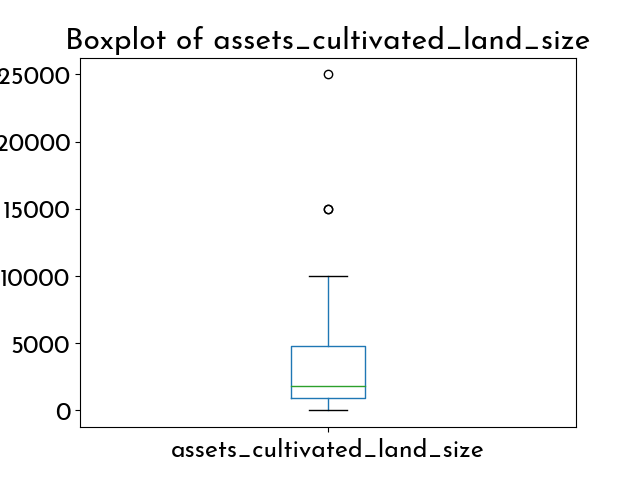
\includegraphics[scale=0.5]{/Users/chaix/Hedera/GIT/XLSform2PDF/output/svf/plots/graph_assets_cultivated_land_size.png}
\end{figure}
\paragraph{Do you own any livestock?}
\  \\Variable name: \texttt{assets\_own\_livestock}\\
Type: single choice\\
\\Total number of answers: 245 (100.0\%)
\\[0.2em] \begin{tabular}{p{4cm}|p{8cm}|p{3cm}}
Choice code & Label & Answers \\
\hline
yes & Yes& \cellcolor{color2}147 (60.0\%)\\
\cellcolor{mygray} no & \cellcolor{mygray}No & \cellcolor{color1}98 (40.0\%)\\
\end{tabular}
\paragraph{Cows}
\  \\Variable name: \texttt{assets\_animals\_cows}\\
Type: integer\\
\\Total number of answers: 58 (23.7\%)
\\[0.2em] \begin{tabular}{p{4cm}|p{8cm}}
Minimum value &0.0 \\
\hline
\cellcolor{mygray} Maximum value & \cellcolor{mygray}3.0 \\
\hline
Variance &0.5411373260738052 \\
\hline
\cellcolor{mygray} Mean value & \cellcolor{mygray}1.0517241379310345 \\
\hline
\end{tabular}
\begin{figure}[H]
\centering
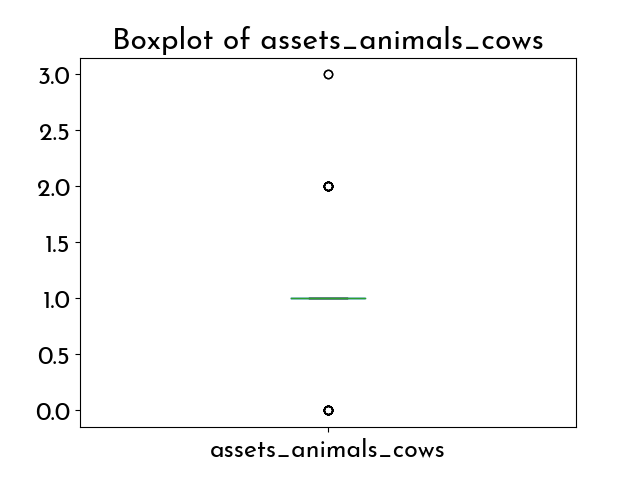
\includegraphics[scale=0.5]{/Users/chaix/Hedera/GIT/XLSform2PDF/output/svf/plots/graph_assets_animals_cows.png}
\end{figure}
\paragraph{Chickens}
\  \\Variable name: \texttt{assets\_animals\_poultry}\\
Type: integer\\
\\Total number of answers: 57 (23.3\%)
\\[0.2em] \begin{tabular}{p{4cm}|p{8cm}}
Minimum value &0.0 \\
\hline
\cellcolor{mygray} Maximum value & \cellcolor{mygray}70.0 \\
\hline
Variance &95.92731829573935 \\
\hline
\cellcolor{mygray} Mean value & \cellcolor{mygray}5.035087719298246 \\
\hline
\end{tabular}
\begin{figure}[H]
\centering
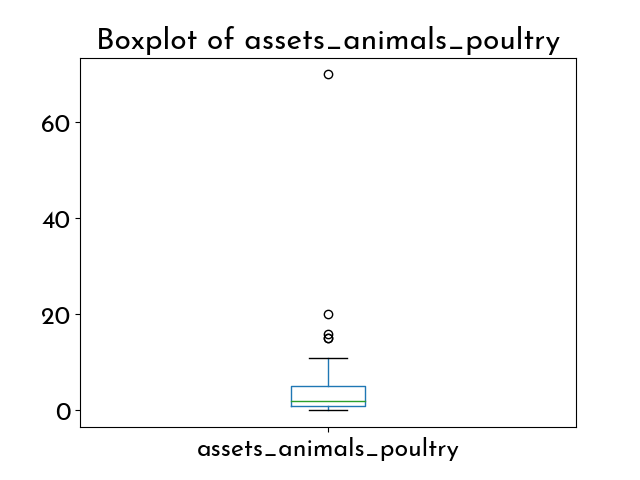
\includegraphics[scale=0.5]{/Users/chaix/Hedera/GIT/XLSform2PDF/output/svf/plots/graph_assets_animals_poultry.png}
\end{figure}
\paragraph{Sheep and goats}
\  \\Variable name: \texttt{assets\_animals\_sheepsgoats}\\
Type: integer\\
\\Total number of answers: 88 (35.9\%)
\\[0.2em] \begin{tabular}{p{4cm}|p{8cm}}
Minimum value &0.0 \\
\hline
\cellcolor{mygray} Maximum value & \cellcolor{mygray}19.0 \\
\hline
Variance &6.230799373040751 \\
\hline
\cellcolor{mygray} Mean value & \cellcolor{mygray}2.352272727272727 \\
\hline
\end{tabular}
\begin{figure}[H]
\centering
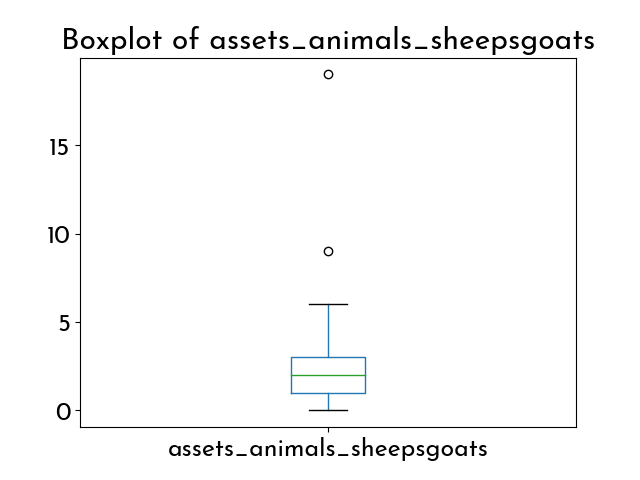
\includegraphics[scale=0.5]{/Users/chaix/Hedera/GIT/XLSform2PDF/output/svf/plots/graph_assets_animals_sheepsgoats.png}
\end{figure}
\paragraph{Pigs}
\  \\Variable name: \texttt{assets\_animals\_pigs}\\
Type: integer\\
\\Total number of answers: 38 (15.5\%)
\\[0.2em] \begin{tabular}{p{4cm}|p{8cm}}
Minimum value &0.0 \\
\hline
\cellcolor{mygray} Maximum value & \cellcolor{mygray}8.0 \\
\hline
Variance &2.967994310099574 \\
\hline
\cellcolor{mygray} Mean value & \cellcolor{mygray}1.2894736842105263 \\
\hline
\end{tabular}
\begin{figure}[H]
\centering
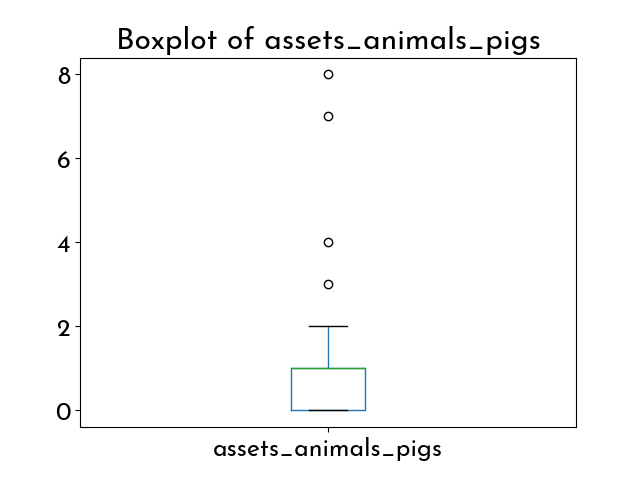
\includegraphics[scale=0.5]{/Users/chaix/Hedera/GIT/XLSform2PDF/output/svf/plots/graph_assets_animals_pigs.png}
\end{figure}
\paragraph{Rabbits}
\  \\Variable name: \texttt{assets\_animals\_rabbits}\\
Type: integer\\
\\Total number of answers: 22 (9.0\%)
\\[0.2em] \begin{tabular}{p{4cm}|p{8cm}}
Minimum value &0.0 \\
\hline
\cellcolor{mygray} Maximum value & \cellcolor{mygray}5.0 \\
\hline
Variance &2.123376623376623 \\
\hline
\cellcolor{mygray} Mean value & \cellcolor{mygray}0.8636363636363636 \\
\hline
\end{tabular}
\begin{figure}[H]
\centering
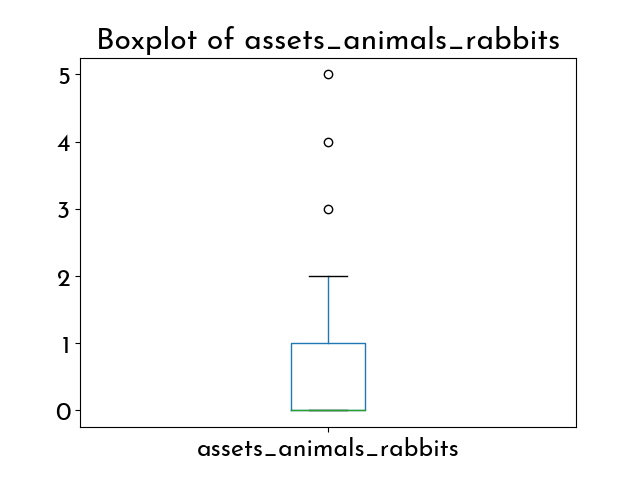
\includegraphics[scale=0.5]{/Users/chaix/Hedera/GIT/XLSform2PDF/output/svf/plots/graph_assets_animals_rabbits.png}
\end{figure}
\paragraph{Other animals}
\  \\Variable name: \texttt{assets\_other\_animal}\\
Type: integer\\
\\Total number of answers: 18 (7.3\%)
\\[0.2em] \begin{tabular}{p{4cm}|p{8cm}}
Minimum value &0.0 \\
\hline
\cellcolor{mygray} Maximum value & \cellcolor{mygray}8.0 \\
\hline
Variance &3.741830065359477 \\
\hline
\cellcolor{mygray} Mean value & \cellcolor{mygray}0.7222222222222222 \\
\hline
\end{tabular}
\begin{figure}[H]
\centering
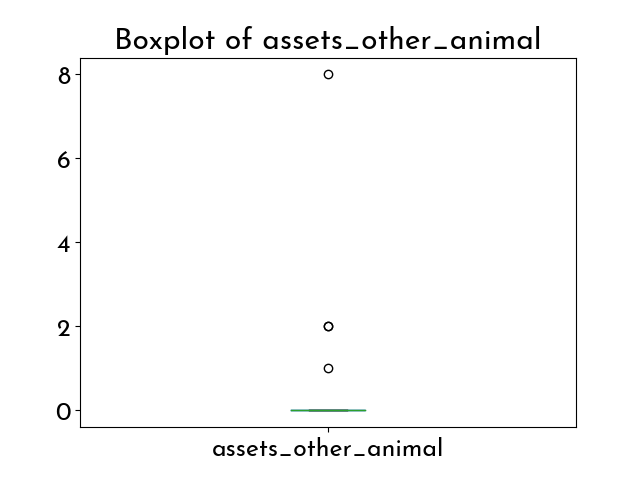
\includegraphics[scale=0.5]{/Users/chaix/Hedera/GIT/XLSform2PDF/output/svf/plots/graph_assets_other_animal.png}
\end{figure}
\paragraph{Please specify:}
\  \\Variable name: \texttt{assets\_other\_animal\_other}\\
Type: text\\
\\Total number of answers: 245 (100.0\%)
\\[0.2em]\begin{table}[H]
 \begin{tabular}{p{4cm}|p{8cm}}
Word & Number of occurrences  \\
\hline
\cellcolor{mygray}chicken&\cellcolor{mygray}1\\
\hline
\end{tabular}
\caption{\label{tab:table-name} Most used words for this answer}
\end{table}
\newpage\section{Willingness to pay}
\paragraph{How much would you be willing and able to pay for a solar system, if you have to pay the total amount upfront?}
\  \\Variable name: \texttt{willingness\_shs\_upfront}\hfill\colorbox{red}{\small{\textcolor{white}{required}}}\\
 Type: single choice\\
\\Total number of answers: 162 (66.1\%)
\\[0.2em] \begin{tabular}{p{4cm}|p{8cm}|p{3cm}}
Choice code & Label & Answers \\
\hline
0\_35000 & Below 35 000 RWF& \cellcolor{color0}9 (5.6\%)\\
\cellcolor{mygray} 35k\_55k & \cellcolor{mygray}35 001 RWF – 55 000 RWF & \cellcolor{color0}10 (6.2\%)\\
55k\_85k & 55 001 RWF – 85 000 RWF& \cellcolor{color0}4 (2.5\%)\\
\cellcolor{mygray} 85k\_105k & \cellcolor{mygray}85 001 RWF – 105 000 RWF & \cellcolor{color0}16 (9.9\%)\\
105k\_200k & 105 001 RWF – 200 000 RWF& \cellcolor{color0}9 (5.6\%)\\
\cellcolor{mygray} 200k\_300k & \cellcolor{mygray}200 001 RWF – 300 000 RWF & \cellcolor{color0}0 (0.0\%)\\
300k\_500k & 300 001  RWF – 500 000 RWF& \cellcolor{color0}0 (0.0\%)\\
\cellcolor{mygray} 500k\_1m & \cellcolor{mygray}500 001 RWF – 1 000 000 RWF & \cellcolor{color0}0 (0.0\%)\\
1m\_2m & 1 000 001 RWF – 2 000 000 RWF& \cellcolor{color0}0 (0.0\%)\\
\cellcolor{mygray} 2m\_above & \cellcolor{mygray}Above 2 000 000 RWF & \cellcolor{color0}0 (0.0\%)\\
afford & I cannot afford any of this, but I would buy if I can pay in instalments& \cellcolor{color2}78 (48.1\%)\\
\cellcolor{mygray} na & \cellcolor{mygray}Do not answer & \cellcolor{color1}36 (22.2\%)\\
\end{tabular}
\paragraph{How much would you be willing to pay per month for a solar system, if you were given 24 months to complete the payment?}
\  \\Variable name: \texttt{willingness\_shs\_loan}\hfill\colorbox{red}{\small{\textcolor{white}{required}}}\\
 Type: single choice\\
\\Total number of answers: 162 (66.1\%)
\\[0.2em] \begin{tabular}{p{4cm}|p{8cm}|p{3cm}}
Choice code & Label & Answers \\
\hline
0\_2500 & 2 500 RWF and below& \cellcolor{color1}57 (35.2\%)\\
\cellcolor{mygray} 2501\_5000 & \cellcolor{mygray}2 501 RWF – 5 000 RWF & \cellcolor{color1}38 (23.5\%)\\
5k\_10k & 5 001 RWF – 10 000 RWF& \cellcolor{color0}14 (8.6\%)\\
\cellcolor{mygray} 10k\_20k & \cellcolor{mygray}10 001 RWF – 20 000 RWF & \cellcolor{color0}1 (0.6\%)\\
20k\_30K & 20 001 RWF – 30 000 RWF& \cellcolor{color0}0 (0.0\%)\\
\cellcolor{mygray} 30k\_50k & \cellcolor{mygray}30 001 RWF – 50 000 RWF & \cellcolor{color0}3 (1.9\%)\\
50k\_above & Above 50 000 RWF& \cellcolor{color0}0 (0.0\%)\\
\cellcolor{mygray} na & \cellcolor{mygray}Do not answer & \cellcolor{color1}49 (30.2\%)\\
\end{tabular}
\paragraph{How much would you be willing and able to pay per month for a storage tank at your house?}
\  \\Variable name: \texttt{willingness\_water\_storage}\hfill\colorbox{red}{\small{\textcolor{white}{required}}}\\
 Type: single choice\\
\\Total number of answers: 202 (82.4\%)
\\[0.2em] \begin{tabular}{p{4cm}|p{8cm}|p{3cm}}
Choice code & Label & Answers \\
\hline
0\_1k & 1 000 RWF and below& \cellcolor{color1}46 (22.8\%)\\
\cellcolor{mygray} 1k\_2k & \cellcolor{mygray}1 000 RWF – 2 000 RWF & \cellcolor{color0}28 (13.9\%)\\
2k\_5k & 2 000 RWF – 5 000 RWF& \cellcolor{color0}38 (18.8\%)\\
\cellcolor{mygray} 5k\_10k & \cellcolor{mygray}5 000 RWF – 10 000 RWF & \cellcolor{color0}27 (13.4\%)\\
10k\_20k & 10 001 RWF – 20 000 RWF& \cellcolor{color0}1 (0.5\%)\\
\cellcolor{mygray} 20k\_30k & \cellcolor{mygray}20 001 RWF – 30 000 RWF & \cellcolor{color0}1 (0.5\%)\\
30k\_above & Above 30 000 RWF& \cellcolor{color0}0 (0.0\%)\\
\cellcolor{mygray} na & \cellcolor{mygray}Do not answer & \cellcolor{color1}61 (30.2\%)\\
\end{tabular}
\paragraph{How much would you be willing and able to pay per month for a safe drinking water source in the village?}
\  \\Variable name: \texttt{willingness\_water\_safety}\hfill\colorbox{red}{\small{\textcolor{white}{required}}}\\
 Type: single choice\\
\\Total number of answers: 162 (66.1\%)
\\[0.2em] \begin{tabular}{p{4cm}|p{8cm}|p{3cm}}
Choice code & Label & Answers \\
\hline
0\_1k & 1 000 RWF and below& \cellcolor{color2}83 (51.2\%)\\
\cellcolor{mygray} 1k\_2k & \cellcolor{mygray}1 000 RWF – 2 000 RWF & \cellcolor{color1}38 (23.5\%)\\
2k\_5k & 2 000 RWF – 5 000 RWF& \cellcolor{color0}21 (13.0\%)\\
\cellcolor{mygray} 5k\_10k & \cellcolor{mygray}5 000 RWF – 10 000 RWF & \cellcolor{color0}5 (3.1\%)\\
10k\_20k & 10 001 RWF – 20 000 RWF& \cellcolor{color0}0 (0.0\%)\\
\cellcolor{mygray} 20k\_30k & \cellcolor{mygray}20 001 RWF – 30 000 RWF & \cellcolor{color0}0 (0.0\%)\\
30k\_above & Above 30 000 RWF& \cellcolor{color0}0 (0.0\%)\\
\cellcolor{mygray} na & \cellcolor{mygray}Do not answer & \cellcolor{color0}15 (9.3\%)\\
\end{tabular}
\end{document}